\chapter{Refinement Types in Practice}\label{chapter:tool}
\makequote
{Everything should be made as simple as possible, but no simpler.}
{Albert Einstein}


\begin{comment}
“One day I will find the right words, and they will be simple.” 
― Jack Kerouac, The Dharma Bums


“Life is really simple, but we insist on making it complicated.” ~ Confucius

“Knowledge is a process of piling up facts; wisdom lies in their simplification.” ~ Martin H. Fischer


“If you can’t explain it to a six year old, you don’t understand it yourself.” ~ Albert Einstein
\end{comment}

\section{Introduction}\label{sec:introduction}

Refinement types enable specification of complex invariants 
by extending the base type system with \emph{refinement predicates} 
drawn from decidable logics. For example,
%
\begin{code}
  type Nat = {v:Int | 0 <= v}
  type Pos = {v:Int | 0 <  v}
\end{code}
%
are refinements of the basic type @Int@ with a logical predicate 
that states the \emph{values} @v@ being described must be 
\emph{non-negative} and \emph{postive} respectively. 
%
We can specify \emph{contracts} of functions by refining function types. 
For example, the contract for @div@
%
\begin{code}
  div :: n:Nat -> d:Pos -> {v:Nat | v <= n}
\end{code}
%
states that @div@ \emph{requires} a non-negative dividend @n@ and a positive
divisor @d@, and \emph{ensures} that the result is less than the dividend.
%
If a program (refinement) type checks, we can be sure that @div@ will never 
throw a divide-by-zero exception.

What are refinement types good for?
%
While there are several papers describing the \emph{theory} behind  
refinement types 
~\cite{Zenger97,pfenningxi98,ORS92,flanagan06,GordonTOPLAS2011,fstar,LiquidPLDI08}, 
even for \toolname~\cite{LiquidICFP14}, there is rather less 
literature on how the approach can be \emph{applied} to large, real-world
codes. In particular, we try to answer the following questions:
%
\begin{enumerate}
  \item What properties can be specified with refinement types?
  \item What inputs are provided and what feedback is received?
  \item What is the process for modularly verifying a library?
  \item What are the limitations of refinement types? 
\end{enumerate}

In this paper, we attempt to investigate these questions, by using the
refinement type checker \toolname, to specify and verify a variety of 
properties of over 10,000 lines of Haskell code from various popular 
libraries, including @containers@, \hbox{@hscolor@,} @bytestring@, @text@, 
@vector-algorithms@ and @xmonad@. 
%
First (\S~\ref{sec:liquidhaskell}), 
we present a high-level overview of \toolname, through a tour 
of its features.
%
Second, we present a qualitative discussion of the kinds of properties
that can be checked -- ranging from generic application independent 
criteria like totality (\S~\ref{sec:totality}), 
\ie that a function is defined for all inputs (of a given type),  
and termination, 
(\S~\ref{sec:termination}) 
\ie that a recursive function cannot diverge,
to application specific concerns like memory safety (\S~\ref{sec:memory-safety}) 
and functional correctness properties (\S~\ref{sec:structures}).
%
Finally (\S~\ref{sec:evaluation}), we present a quantitative evaluation of the approach, with a view
towards measuring the efficiency and programmer's effort required for
verification, 
and we discuss various limitations of the approach which could
provide avenues for further work.


%%% Local Variables: 
%%% mode: latex
%%% TeX-master: "main"
%%% End: 

\section{\toolname}\label{sec:liquidhaskell}
\begin{figure*}[ht!]
\noindent\makebox[\textwidth]{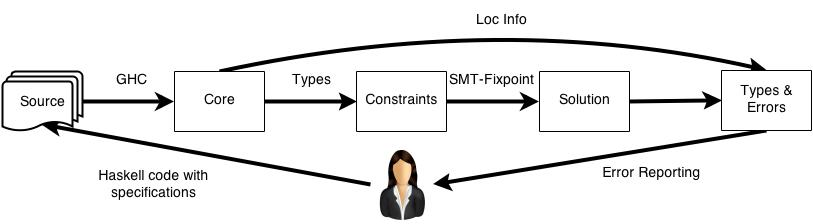
\includegraphics[width=\textwidth]{text/realworldhaskell/liquidHaskell}}
\caption{\toolname Workflow}
	\label{fig:internals}
\end{figure*}
% 
% link for workflow
% https://www.draw.io/#G0Bwp_mIorSVqJb2RENnNVWVlQTmc
%
We will start with a short description of the \toolname workflow,
summarized in Figure~\ref{fig:internals}, and continue with an 
example driven overview of how properties are specified
and verified using the tool. 

% \mypara{Usage} 
\mypara{Source}
\toolname can be run from the command-line\footnote{\url{https://hackage.haskell.org/package/liquidhaskell}}
or within a web-browser\footnote{\url{http://goto.ucsd.edu/liquid/haskell/demo/}}.
It takes as \emph{input}:
%
(1)~a single Haskell \emph{source} file with code and refinement
    type specifications including refined datatype definitions, 
    measures (\S~\ref{sec:tool:measures}), predicate and type 
    aliases, and function signatures;
%
(2)~a set of directories containing \emph{imported modules} 
    (including the \verb+Prelude+) which may themselves 
    contain specifications for exported types and functions; and
%
(3)~a set of predicate fragments called \emph{qualifiers},
    which are used to infer refinement types. This set is 
    typically empty as the default set of qualifiers extracted 
    from the type specifications suffices for inference.

\mypara{Core}
\toolname uses GHC to reduce the source to the Core IL~\cite{SulzmannCJD07}, 
and, to facilitate source-level error reporting, creates a map from Core 
expressions to locations in the Haskell source.

\mypara{Constraints}
Then, it uses the abstract interpretation framework of Liquid Typing~\cite{LiquidPLDI08}, 
modified to ensure soundness under lazy evaluation~\citep{LiquidICFP14},
to generate logical constraints from the Core IL.
     
\mypara{Solution}
Next, it uses a fixpoint algorithm (from~\citep{LiquidPLDI08})
combined with an SMT solver to solve the constraints, and hence 
infers a valid refinement typing for the program. 
%
\toolname can use any solver that implements the SMT-LIB2
standard~\cite{SMTLIB2}, including Z3~\citep{Z3}, CVC4~\citep{CVC4}, and
MathSat~\citep{MathSat}.

 
\mypara{Types \& Errors}
% \NV{satisfiability and validity refer to different things here, 
% which is confusing...}
If the set of constraints is satisfiable, then \toolname outputs 
\textsc{Safe}, meaning the program is verified.
If instead, the set of constraints is not satisfiable, then \toolname
outputs \textsc{Unsafe}, and uses the invalid constraints to 
report refinement type errors at the \emph{source positions}
that created the invalid constraints, using the location 
information to map the invalid constraints to source positions.
%
In either case, \toolname produces as output a source map
containing the \emph{inferred} types for each program 
expression, which, in our experience, is crucial for 
debugging the code and the specifications.

%\mypara{Optional Typing}
%
\toolname is best thought of as an \emph{optional} type checker
for Haskell. By optional we mean that the refinements have \emph{no} 
influence on the dynamic semantics, which makes it easy to apply 
\toolname to \emph{existing} libraries.
%
To emphasize the optional nature of refinements and preserve 
compatibility with existing compilers, all specifications 
appear within comments of the form \verb|{-@ ... @-}|, 
which we omit below for brevity.

\subsection{Specifications}

A refinement type is a Haskell type where each component
of the type is decorated with a predicate from a (decidable)
refinement logic. We use the quantifier-free logic of equality, 
uninterpreted functions and linear arithmetic (QF-EUFLIA)~\cite{Nelson81}. 
For example,
%
\begin{code}
   {v:Int | 0 <= v && v < 100}
\end{code}
%
describes @Int@ values between @0@ and @100@.

\mypara{Type Aliases} For brevity and readability, it is often convenient 
to define abbreviations for particular refinement predicates and types.
For example, we can define an alias for the above predicate
%
\begin{code}
  predicate Btwn Lo N Hi = Lo <= N && N < Hi
\end{code}
%
and use it to define a \emph{type alias}
%
\begin{code}
  type Rng Lo Hi = {v:Int | (Btwn Lo v Hi)} 
\end{code}
%
We can now describe the above integers as @(Rng 0 100)@.

\mypara{Contracts} 
To describe the desired properties of a function, we need
simply refine the input and output types with predicates 
that respectively capture suitable pre- and post-conditions. 
For example,
%
\begin{code}
  range :: lo:Int -> hi:{Int | lo <= hi} 
        -> [(Rng lo hi)]
\end{code}
%
states that @range@ is a function that takes two @Int@s 
respectively named @lo@ and @hi@ and returns a list of @Int@s 
between @lo@ and @hi@. There are three things worth
noting.
%
First, we have binders to name the function's \emph{inputs} 
(\eg, @lo@ and @hi@) and can use the binders inside the 
function's \emph{output}.
%
Second, the refinement in the \emph{input} type describes the 
\emph{pre-condition} that the second parameter @hi@ cannot 
be smaller than the first @lo@.
%
Third, the refinement in the \emph{output} type describes the
\emph{post-condition} that all returned elements are between 
the bounds of @lo@ and @hi@.


\subsection{Verification}\label{sec:tool:verification}

Next, consider the following implementation for @range@:
%
\begin{code}
  range lo hi 
    | lo <= hi  = lo : range (lo + 1) hi
    | otherwise = []
\end{code}
%
When we run \toolname on the above code, it reports an 
error at the definition of @range@. This is unpleasant! 
One way to debug the error is to determine what type has
been \emph{inferred} for @range@, \eg, by hovering the 
mouse over the identifier in the web interface. 
In this case, we see that the output type is essentially:
%
\begin{code}
  [{v:Int | lo <= v && v <= hi}]
\end{code}
%
which indicates the problem. There is an \emph{off-by-one} 
error due to the problematic guard. If we replace the second @<=@ 
with a @<@ and re-run the checker, the function is verified.

\mypara{Holes} It is often cumbersome to specify the Haskell
types, as those can be gleaned from the regular type signatures 
or via GHC's inference. Thus, \toolname allows the user to leave 
holes in the specifications. Suppose @rangeFind@ has type 
%
\begin{code}
  (Int -> Bool) -> Int -> Int -> Maybe Int
\end{code}
%
where the second and third parameters define a range. 
We can give @rangeFind@ a refined specification:
%
\begin{code}
  _ -> lo:_ -> hi:{Int | lo <= hi} 
    -> Maybe (Rng lo hi)
\end{code}
%
where the @_@ is simply the unrefined Haskell type for the 
corresponding position in the type.

\mypara{Inference} Next, consider the implementation
%
\begin{code}
  rangeFind f lo hi = find f $ range lo hi 
\end{code}
%$
where @find@ from @Data.List@ has the (unrefined) type
%
\begin{code}
  find :: (a -> Bool) -> [a] -> Maybe a
\end{code}
%
\toolname uses the abstract interpretation framework of 
Liquid Typing~\cite{LiquidPLDI08} to infer that the type
parameter @a@ of @find@ can be instantiated with @(Rng lo hi)@
thereby enabling the automatic verification of @rangeFind@.

Inference is crucial for automatically synthesizing types
for polymorphic instantiation sites -- note there is another
instantiation required at the use of the apply operator 
@$@ --  and to relieve the programmer of the tedium of %$
specifying signatures for all functions. 
%
Of course, for functions exported by the module,
we must write signatures to specify preconditions -- otherwise, 
the system defaults to using the trivial (unrefined) Haskell 
type as the signature \ie, checks the implementation assuming 
arbitrary inputs.

\subsection{Measures}\label{sec:tool:measures}
%% \NV{DONE(R1)
%% measure is introduced as something that gives the size of a value, 
%% but it is later used for more general properties e.g. almostRB 
%% over red-black trees.
%% }
So far, the specifications have been limited to comparisons and 
arithmetic operations on primitive values. 
We use \emph{measure functions}, or just measures, to 
specify \emph{inductive properties} of algebraic data types. 
%
For example, we define a measure @len@ to write properties about the number
of elements in a list.
%
\begin{code}
  measure len :: [a] -> Int
  len []      = 0
  len (x:xs)  = 1 + (len xs)
\end{code}
%
Measure definitions are \emph{not} arbitrary Haskell code but a very 
restricted subset~\cite{LiquidICFP14}.
Each measure has a single equation per constructor that defines the
value of the measure for that constructor. The right-hand side of the 
equation is a term in the restricted refinement logic. Measures are 
interpreted by generating refinement types for the corresponding 
data constructors.
%
For example, from the above, \toolname derives the 
following types for the list data constructors:
%
\begin{code}
  []  :: {v:[a]| len v = 0}
  (:) :: _ -> xs:_ -> {v:[a]| len v = 1 + len xs}
\end{code}
%
Here, @len@ is an \emph{uninterpreted function} in the refinement logic.
We can define multiple measures for a type; \toolname simply conjoins
the individual refinements arising from each measure to obtain a single
refined signature for each data constructor.

\mypara{Using Measures}
We use measures to write specifications about algebraic types. 
For example, we can specify and verify that: 
%
\begin{code}
  append :: xs:[a] -> ys:[a] 
         -> {v:[a]| len v = len xs + len ys}

  map    :: (a -> b) -> xs:[a] 
         -> {v:[b]| len v = len xs} 

  filter :: (a -> Bool) -> xs:[a] 
         -> {v:[a]| len v <= len xs}
\end{code}

\mypara{Propositions} 
%%In addition to allowing the specification of structural features like
%%lengths, heights and so on, 
Measures can be used to encode sophisticated 
invariants about algebraic data types.
%
To this end, the user can write a measure whose output has a special type 
@Prop@ denoting propositions in the refinement logic. For instance, we can
describe a list that contains a @0@ as:
%
\begin{code}
  measure hasZero :: [Int] -> Prop
  hasZero []      = false
  hasZero (x:xs)  = x == 0 || (hasZero xs) 
\end{code}
%
We can then define lists containing a @0@ as:
%
\begin{code}
  type HasZero = {v : [Int] | (hasZero v)} 
\end{code}
%
Using the above, \toolname will accept 
%
\begin{code}
  xs0 :: HasZero 
  xs0 = [2,1,0,-1,-2]
\end{code}
%
but will reject
%
\begin{code}
  xs' :: HasZero 
  xs' = [3,2,1]
\end{code}



\subsection{Refined Data Types}

Often, we require that \emph{every} instance of a type satisfies some invariants. 
For example, consider a @CSV@ data type, that represents tables:
%
\begin{code}
  data CSV a = CSV { cols :: [String]
                   , rows :: [[a]]    }
\end{code}
%
% With \toolname we can enforce the invariant that for every @CSV@ table, 
% with a number of columns given by @dim@,
% each row has @dim@ elements,
% with the below refined data type definition
%%With \toolname we can enforce the invariant that every @CSV@ table 
%%has the number of columns given by @dim@, and that each row has 
%%@dim@ elements with a refined data type definition, such as:
With \toolname we can enforce the invariant that every row in a @CSV@ table
should have the same number of columns as there are in the header
%
\begin{code}
  data CSV a = CSV { cols :: [String]  
                   , rows :: [ListL a cols] }
\end{code}
%
using the alias
%
\begin{code}
  type ListL a X = {v:[a]| len v = len X}
\end{code}
%
A refined data definition is \emph{global} in that \toolname 
will reject any @CSV@-typed expression that does not respect 
the refined definition. For example, both of the below 
%
\begin{code}
  goodCSV = CSV [  "Month", "Days"] 
                [ ["Jan"  , "31"]
                , ["Feb   , "28"]
                , ["Mar"  , "31"] ]

  badCSV  = CSV [  "Month", "Days"] 
                [ ["Jan"  , "31"]
                , ["Feb   , "28"]
                , ["Mar"        ] ]
\end{code}
%
are well-typed Haskell, but the latter is rejected by \toolname.
%
Like measures, the global invariants are enforced by refining 
the constructors' types. 

\subsection{Refined Type Classes}\label{sec:type-classes}

Next, let us see how \toolname supports the verification of
programs that use ad-hoc polymorphism via type classes.
%
While the implementation of each typeclass instance is 
different, there is often a common interface that we 
expect all instances to satisfy.

\mypara{Class Measures}
As an example, consider the class definition
%
\begin{code}
  class Indexable f where
    size :: f a -> Int
    at   :: f a -> Int -> a
\end{code}
%
For safe access, we might require that @at@'s second 
parameter is bounded by the @size@ of the container.
To this end, we define a \emph{type-indexed} 
measure, using the @class measure@ keyword
%
\begin{code}
  class measure sz :: a -> Nat
\end{code}
%
Now, we can specify the safe-access precondition  
independent of the particular instances of @Indexable@:
%
\begin{code}
  class Indexable f where
    size :: xs:_ -> {v:Nat | v = sz xs}
    at   :: xs:_ -> {v:Nat | v < sz xs} -> a
\end{code}

\mypara{Instance Measures}
For each concrete type that instantiates a class, we require 
a corresponding definition for the measure. 
For example, to define lists as an instance of @Indexable@, 
we require the definition of the @sz@ instance for lists:
%
\begin{code}
  instance measure sz :: [a] -> Nat
  sz []     = 0
  sz (x:xs) = 1 + (sz xs)
\end{code}
%
Class measures work just like regular measures in that the above 
definition is used to refine the types of the list data constructors.
After defining the measure, we can define the type instance as:
%
\begin{code}
  instance Indexable [] where
    size []        = 0
    size (x:xs)    = 1 + size xs

    (x:xs) `at` 0  = x
    (x:xs) `at` i  = index xs (i-1)
\end{code}
%
\toolname uses the definition of @sz@ for lists to check that @size@ 
and @at@ satisfy the refined class specifications. 
% NV the dictionary relevant this were removed
% , and hence, that 
% the above creates a valid instance dictionary for @Indexable@.

\mypara{Client Verification}
At the clients of a type-class we use the refined 
types of class methods. Consider a client of @Indexable@s:
%
\begin{code}
  sum :: (Indexable f) => f Int -> Int
  sum xs = go 0 
    where
      go i | i < size xs = xs `at` i + go (i+1)
           | otherwise   = 0
\end{code}
%
\toolname proves that each call to @at@ is safe, by using the refined
class specifications of @Indexable@. 
Specifically, each call to @at@ is guarded by a check @i < size xs@
and @i@ is  increasing 
from 0, so \toolname proves that @xs `at` i@ will always be safe.

\subsection{Abstracting Refinements}

So far, all the specifications have used \emph{concrete} refinements. Often it is
useful to be able to \emph{abstract} the refinements that appear in a
specification. For example, consider a monomorphic variant of @max@
%
\begin{code}
  max     :: Int -> Int -> Int 
  max x y = if x > y then x else y
\end{code}
%
We would like to give @max@ a specification that lets us verify:
%
\begin{code}
  xPos  :: {v: _ | v > 0}
  xPos  = max 10 13

  xNeg  :: {v: _ | v < 0}
  xNeg  = max (-5) (-8)

  xEven :: {v: _ | v mod 2 == 0} 
  xEven = max 4 (-6)
\end{code}
%
To this end, \toolname allows the user to \emph{abstract refinements} over
types~\cite{vazou13}, for example by typing @max@ as:
%
\begin{code}
 max :: forall <p :: Int -> Prop>. 
          Int<p> -> Int<p> -> Int<p>
\end{code}
%
The above signature states that for any refinement @p@, if the two
inputs of @max@ satisfy @p@ then so does the output. \toolname uses
Liquid Typing to automatically instantiate @p@ with suitable concrete
refinements, thereby checking @xPos@, @xNeg@, and @xEven@.


\mypara{Dependent Composition}
Abstract refinements turn out to be a surprisingly expressive and 
useful specification mechanism. For example, consider the function 
composition operator:
%
\begin{code}
  (.) :: (b -> c) -> (a -> b) -> a -> c
  (.) f g x = f (g x)  
\end{code}
%
Previously, it was not possible to check, \eg that:
%
\begin{code}
  plus3 :: x:_ -> {v:_ | v = x + 3}
  plus3 = (+ 1) . (+ 2)
\end{code}
%
as the above required tracking the dependency between @a@, @b@ and @c@,
which is crucial for analyzing idiomatic Haskell.
With abstract refinements, we can give the @(.)@ operator the type:
%
\begin{code}
  (.) :: forall < p :: b -> c -> Prop
                , q :: a -> b -> Prop>.
           f:(x:b -> c<p x>) 
        -> g:(x:a -> b<q x>) 
        -> y:a 
        -> exists[z:b<q y>].c<p z>
\end{code}
%
which gets automatically instantiated at usage sites, allowing \toolname
to precisely track invariants through the use of the ubiquitous 
higher-order operator.

\mypara{Dependent Pairs}
Similarly, we can abstract refinements over the definition of datatypes.
% Similarly, we can abstract refinements over the definition of datatypes.
For example, we can express dependent pairs in \toolname by refining the 
definition of tuples as:
%
\begin{code}
  data Pair a b <p :: a -> b -> Prop> 
    = Pair { fst :: a, snd :: b<p fst>}
\end{code}
%
That is, the refinement @p@ relates the @snd@ element with the @fst@.
Now we can define increasing and decreasing pairs
%
\begin{code}
  type IncP = Pair <{\x y -> x < y}> Int Int
  type DecP = Pair <{\x y -> x > y}> Int Int
\end{code}
%
and then verify that:
%
\begin{code}
  up :: IncP
  up = Pair 2 5
  
  dn :: DecP
  dn = Pair 5 2
\end{code}
%
Now that we have a bird's eye view of the various specification mechanisms
supported by \toolname, let us see how we can profitably apply them to
statically check a variety of correctness properties in real-world codes.

%%% Local Variables: 
%%% mode: latex
%%% TeX-master: "main"
%%% End: 

\section{Totality}\label{sec:totality}
%% OK \NV{DONE intro (R1)
%% OK Sections 3 and 4 cover "totality" and "termination" respectively. It would be helpful to explain these terms at the start of section 3, so that the two are distinguished appropriately.
%% OK }
Well typed Haskell code can go very wrong:
%
\begin{code}
  *** Exception: Prelude.head: empty list
\end{code}
%
As our first application, let us see how to use 
\toolname to statically guarantee the absence
of such exceptions, \ie, to prove various 
functions \emph{total}.

\subsection{Specifying Totality}

First, let us see how to specify the notion of
totality inside \toolname. Consider the source of 
the above exception:
%
\begin{code}
  head :: [a] -> a
  head (x:_) = x
\end{code}
%
Most of the work towards totality checking is done by 
the translation to GHC's Core, in which every function 
\emph{is} total, but may explicitly call an \emph{error} 
function that takes as input a string that describes the 
source of the pattern-match failure and throws an exception.
%
For example @head@ is translated into
%
\begin{code}
  head d = case d of 
             x:xs -> x
             []   -> patError "head"
\end{code}

Since every core function is total, but may explicitly 
call error functions, to prove that the source function is 
total, it suffices to prove that @patError@ 
will \emph{never} be called.
%
We can specify this requirement by giving the error 
functions a @false@ pre-condition:
%
\begin{code}
  patError :: {v:String | False } -> a
\end{code}
%
The pre-condition states that the input type is \emph{uninhabited}
and so an expression containing a call to @patError@ will only type 
check if the call is \emph{dead code}.


\subsection{Verifying Totality}

The (core) definition of @head@ does not typecheck
as is; but requires a pre-condition that states that the function
is only called with non-empty lists. Formally, we do so by 
defining the alias
%
\begin{code}
  predicate NonEmp X = 0 < len X 
\end{code}
%
and then stipulating that 
%
\begin{code}
  head :: {v : [a] | NonEmp v} -> a
\end{code}
%
To verify the (core) definition of @head@, \toolname uses the above signature
to check the body in an environment
%
\begin{code}
  d :: {0 < len d}
\end{code}
%
When @d@ is matched with @[]@, the environment is 
strengthened with the corresponding refinement from 
the definition of @len@, \ie,
%
\begin{code}
  d :: {0 < (len d) && (len d) = 0}
\end{code}
%
Since the formula above is a contradiction, \toolname concludes that the
call to @patError@ is dead code, and thereby verifies the totality 
of @head@. Of course, now we have pushed the burden of proof onto clients
of @head@ -- at each such site, \toolname will check that the argument 
passed in is indeed a @NonEmp@ list, and if it successfully does so, then
we, at any uses of @head@, can rest assured that @head@ will never throw an 
exception. 

\mypara{Refinements and Totality} 
While the @head@ example is quite simple, in general, refinements make
it easy to prove totality in complex situations, where we must track
dependencies between inputs and outputs. For example, consider the @risers@
function from \cite{catch}:
%
\begin{code}
  risers []       = []
  risers [x]      = [[x]]
  risers (x:y:zs) 
    | x <= y      = (x:s) : ss 
    | otherwise   = [x] : (s:ss) 
    where 
      s:ss    = risers (y:etc)
\end{code}
%
The pattern match on the last line is partial; its core translation is
%
\begin{code}
  let (s, ss) = case risers (y:etc) of
                  s:ss -> (s, ss)
                  []   -> patError "..."
\end{code}
%
What if @risers@ returns an empty list? 
Indeed, @risers@ \emph{does}, on occasion, return an empty list per its
first equation. However, on close inspection, it turns out that 
\emph{if} the input is non-empty, \emph{then} the output is also
non-empty. Happily, we can specify this as:
%
\begin{code}
  risers :: l:_ -> {v:_ | NonEmp l => NonEmp v} 
\end{code}

\toolname verifies that @risers@ meets the above specification, 
and hence that the @patError@ is dead code as at that 
site, the scrutinee is obtained from calling @risers@ with a
@NonEmp@ list.

\mypara{Non-Emptiness via Measures}
Instead of describing non-emptiness indirectly using @len@, a 
user could a special measure:
%
\begin{code}
  measure nonEmp  :: [a] -> Prop
  nonEmp (x:xs)   = True
  nonEmp []       = False

  predicate NonEmp X = nonEmp X
\end{code}
%
After which, verification would proceed analagous to the above.

\mypara{Total Totality Checking} 
@patError@ is one of many possible errors thrown by non-total functions.  
@Control.Exception.Base@ has several others including @recSelError@, @irrefutPatError@, \etc which serve the purpose of making 
core translations total.
%
Rather than hunt down and specify @False@ preconditions one
by one, the user may automatically turn on totality checking 
by invoking \toolname with the \cmdtotality command line option, 
at which point the tool systematically checks that all the above 
functions are indeed dead code, and hence, that all definitions are total.

\subsection{Case Studies}

We verified totality of two libraries: \lbhscolour and \lbmap, earlier versions
of which had previously been proven total by \texttt{catch}~\citep{catch}.

\mypara{\lbmap} 
is a widely used library for (immutable) key-value maps, implemented
as balanced binary search trees.
Totality verification of \lbmap was quite straightforward.
We had already verified termination and the crucial 
binary search invariant~\ref{chapter:abstractrefinements}. To verify 
totality it sufficed to simply re-run verification with
the \cmdtotality argument.
%
All the important specifications were already captured by the types, 
and no additional changes were needed to prove totality.
%
%% \RJ{was it trivially total? i.e. is it total if you strip out all refinements
%% from specs?}
%% \NV{No, it fails in 6 functions all of which can trivially be reasoned to be total}
%% \NV{hedgeUnion, hedgeDiff, hedgeMerge, submap', join, merge}
%% \NV{The interesting story is that during verification \emph{we accidentally modified}
%% turn a function to partial, see my commit 041f1f0fea4d34ee41f50dbf7ce43e3c084c2743}
%

This case study illustrates an advantage of \toolname over specialized provers 
(\eg, \texttt{catch}~\citep{catch}): it can be used to prove totality, termination and
functional correctness at the same time, facilitating a nice reuse of
specifications for multiple tasks.

%% DONE \NV{(R3)
%% DONE Before discussing HsColour, I'd give a brief explanation of what it is.
%% DONE }
\mypara{\lbhscolour} is a library for generating syntax-highlighted LATEX and HTML from
Haskell source files.
Checking \lbhscolour was not so easy, as in some cases assumptions are used about the 
structure of the input data:
%
For example, @ACSS.splitSrcAndAnnos@ handles an
input list of @String@s and assumes that whenever
a specific @String@ (say @breakS@) appears then 
at least two @String@s (call them @mname@ and @annots@)
follow it in the list.
Thus, for a list @ls@ that starts with @breakS@ 
the irrefutable pattern  @(_:mname:annots)@ @=@ @ls@
should be total.
%
Though possible, it is currently it is somewhat cumbersome to specify such 
properties. 
%
As an easy and practical solution, 
to prove totality, we added a dynamic check that 
validates that the length of the input @ls@ exceeds @2@.

%% measure follows a b c = \case 
%%   []   -> true
%%   x:xs -> if x == a then first2 b c xs else follows a b c xs
%% 
%% measure first2 b c = \case
%%   []   -> false
%%   x:xs -> x == b && first1 c xs
%% 
%% measure first1 c = \case
%%   []   -> false
%%   x:xs -> x == c
%% 
%% Worse, \toolname has no way to express such an invariant: 
%% \toolname naturally describes invariants that recursively 
%% hold for every list element and 
%% reaches its limitations when reasoning about non-recursive
%% properties.

In other cases assertions were imposed via monadic checks, \eg @HsColour.hs@ reads the input arguments and 
checks their well-formedness using 
%
\begin{code}
  when (length f > 1) $ errorOut "..."
\end{code} %$
%
Currently \toolname does not support monadic reasoning that 
allows assuming that @(length f <= 1)@
holds when executing the action \emph{following} the @when@ check. 
%
Finally, code modifications were required to capture properties 
that are cumbersome to express with \toolname.
%
For example, @trimContext@ checks if there is an element that 
satisfies @p@ in the list @xs@; if so it defines 
%
@ys = dropWhile (not . p) xs@
%
and computes @tail ys@.
%
By the check we know that @ys@ has at least one element, the 
one that satisfies @p@. 
%
Due to the complexity of this property, we preferred to rewrite the specific code 
in a more verification friendly version. 


%%% \mynote{Bug}
%%% %
%%% \RJ{WHY? Seems like a simple GHC CHECK?}
%%% %
%%% On the positive side, totality verification revealed a subtle bug:
%%% %
%%% The instance @Enum@ of @Highlight@ does not define the @toEnum@ 
%%% method. In core, this reduces to a call to the error function 
%%% @noMethodBinding@.
%%% %
%%% Even though this totality bug can be tracked by GHC compilation,
%%% it exposes the strengths of our totality checker.

On the whole, while proving totality can be cumbersome 
(as in \lbhscolour) it is a nice side benefit of refinement
type checking and can sometimes be a fully automatic corollary
of establishing more interesting safety properties (as in \lbmap).

\section{Termination}\label{sec:termination}

To soundly account for Haskell's non-strict evaluation, a refinement
type checker must distinguish between terms that may potentially 
diverge and those that will not~\cite{LiquidICFP14}.
%
Thus, by default, \toolname proves termination of each recursive function.
Fortunately, refinements make this onerous task quite straightforward. 
We need simply associate a \emph{well-founded termination metric} % $\mu$
on the function's parameters, and then use refinement typing to check 
that the metric strictly decreases at each recursive call. In practice,
due to a careful choice of defaults, this amounts to about a line 
of termination-related hints per hundred lines of source. 
Details about the termination checker may be found in \cite{LiquidICFP14}, 
we include a brief description here to make the paper self-contained.

\mypara{Simple Metrics}
As a starting example, consider the @fac@ function
%
\begin{code}
  fac :: n:Nat -> Nat / [n]
  fac 0 = 1 
  fac n = n * fac (n-1)
\end{code}
%
The termination metric is simply the parameter @n@; 
as @n@ is non-negative and decreases at the recursive 
call, \toolname verifies that @fac@ will terminate.
%
We specify the termination metric in the type signature 
with the @/[n]@.

Termination checking is performed at the same 
time as regular type checking, as it can be 
reduced to refinement type checking with a 
special terminating fixpoint combinator~\cite{LiquidICFP14}.
Thus, if \toolname fails to prove that a given 
termination metric is well-formed and decreasing, 
it will report a @Termination Check@ @Error@. 
%% \RJ{Seems untrue -- I just get a plain old liquid type error?
%% NV: IF you provide termination metrics, you DO get termination check error}.
At this point, the user can either debug 
the specification, or mark the function 
as non-terminating.


%%\mypara{Refinements Enable Termination} 
%%Consider Euclid's GCD:
%%%
%%\begin{code}
%%  gcd :: a:Nat -> {v:Nat | v < a} -> Nat 
%%  gcd a 0 = a
%%  gcd a b = gcd b (a `mod` b)
%%\end{code}
%%%
%%Here, the termination metric is the first parameter @a@.
%%To prove that @a@ is decreasing requires
%%the fact that the second parameter is smaller than the first 
%%and that @mod@ returns results smaller than its second 
%%parameter. Both facts are easily expressed as refinements, 
%%but elude non-extensible checkers~\cite{Giesl11}.
%%
%%\mypara{Explicit Termination Metrics}
%%The termination metric can be some parameter \emph{other} than the first 
%%argument.
%%For example, consider: % As an example, consider the tail-recursive factorial:
%%%
%%\begin{code}
%%  tfac     :: Nat -> n:Nat -> Nat / [n] 
%%  tfac x 0 = if n == 0 then x
%%                       else tfac (n*x) (n-1)
%%\end{code}
%%%
%%%
%%It can be checked that @n@, \ie, the second argument is decreasing at each recursive call.
%%
\mypara{Termination Expressions} 
Sometimes, no single parameter decreases across recursive calls,
but there is some \emph{expression} that forms the decreasing 
metric.
%
For example recall @range lo hi@ (from \S~\ref{sec:tool:verification}) 
which returns the list of @Int@s from @lo@ to @hi@:
%
\begin{code}
  range lo hi 
    | lo < hi   = lo : range (lo+1) hi
    | otherwise = [] 
\end{code}
%
Here, neither parameter is decreasing (indeed, the first 
one is increasing) but @hi-lo@ decreases across each call. 
To account for such cases, we can specify as the termination
metric a (refinement logic) expression over the function
parameters. Thus, to prove termination, we could type @range@ as:
\begin{code}
  lo:Int -> hi:Int -> [(Btwn lo hi)] / [hi-lo]
\end{code}

\mypara{Lexicographic Termination}
The Ackermann function
%
\begin{code}
  ack m n 
    | m == 0    = n + 1
    | n == 0    = ack (m-1) 1 
    | otherwise = ack (m-1) (ack m (n-1))
\end{code}
%
is curious as there exists no simple, natural-valued, 
termination metric that decreases at each recursive call.
%
However @ack@ terminates because at each call \emph{either}
@m@ decreases \emph{or} @m@ remains the same and @n@ decreases. 
%
In other words, the pair @(m,n)@ strictly decreases according to a
\emph{lexicographic} ordering. 
%
Thus \toolname supports termination metrics that are a 
\emph{sequence of} termination expressions. For example, 
we can type @ack@ as:
%
\begin{code}
  ack :: m:Nat -> n:Nat -> Nat / [m, n]
\end{code}
%
At each recursive call \toolname uses a lexicographic 
ordering to check that the sequence of termination 
expressions is decreasing (and well-founded in each component).

\mypara{Mutual Recursion}
%
The lexicographic mechanism lets us check termination of
mutually recursive functions, \eg @isEven@ and @isOdd@
%
\begin{code}
  isEven 0 = True
  isEven n = isOdd $ n-1
  
  isOdd n  = not $ isEven n 
\end{code}
%
Each call terminates as either @isEven@ calls @isOdd@ with a 
decreasing parameter, \emph{or} @isOdd@ calls @isEven@ with 
the same parameter, expecting the latter to do the decreasing.
%
For termination, we type:
%
\begin{code}
  isEven :: n:Nat -> Bool / [n, 0]
  isOdd  :: n:Nat -> Bool / [n, 1]
\end{code}
%
To check termination, \toolname verifies that at each recursive 
call the metric of the caller is less than the metric of the 
callee.
%
When @isEven@ calls @isOdd@, it proves that the caller's 
metric, namely @[n,0]@ is greater than the callee's @[n-1,1]@.
When \hbox{@isOdd@} calls @isEven@, it proves that the 
caller's metric @[n,1]@ is greater than the callee's @[n,0]@,
thereby proving the mutual recursion always terminates.

\mypara{Recursion over Data Types}
The above strategies generalize easily to functions that recurse
over (finite) data structures like arrays, lists, and trees.
In these cases, we simply use \emph{measures} to project the 
structure onto @Nat@, thereby reducing the verification to 
the previously seen cases. 
For example, we can prove that @map@ 
%
\begin{code}
  map f (x:xs) = f x : map f xs
  map f []     = []
\end{code}
%
terminates, by typing @map@ as 
%
\begin{code}
  (a -> b) -> xs:[a] -> [b] / [len xs]
\end{code}
%
\ie, by using the measure @len xs@, from \S~\ref{sec:tool:measures}, 
as the metric.

%%% %
%%% \begin{code}
%%%   data L [sz] a = N | C a (L a)
%%% \end{code}
%%% %
%%% we can define a \emph{measure}
%%% %
%%% \begin{code}
%%%   measure sz  :: L a -> Nat
%%%   sz (C x xs) = 1 + (sz xs)
%%%   sz N        = 0
%%% \end{code}
%%% %
%%% We prove that @map@ terminates using the type:
%%% %
%%% \begin{code}
%%%   map :: (a -> b) -> xs:L a -> L b / [sz xs]
%%%   map f (C x xs) = C (f x) (map f xs)
%%%   map f N        = N
%%% \end{code}
%%% %
%%% That is, by simply using @(sz xs)@  as the 
%%% decreasing metric.

\mypara{Generalized Metrics Over Datatypes}
In many functions there is no single argument 
whose measure provably decreases. Consider
%
\begin{code}
  merge (x:xs) (y:ys)
    | x < y     = x : merge xs (y:ys)
    | otherwise = y : merge (x:xs) ys
\end{code}
%
from the homonymous sorting routine. Here, neither
parameter decreases, but the \emph{sum} of their 
sizes does. To prove termination, we can type @merge@ as:
%
\begin{code}
  xs:[a] -> ys:[a] -> [a] / [len xs + len ys]
\end{code}

%%%% \begin{figure*}[!t]
%%%% 	\begin{code}
%%%% 	type OL  a   =  [a]<{\fld v -> (v >= fld)}>
%%%% 
%%%% 	qsort :: (Ord a) => xs:[a] -> OL a / [(len xs), 0]
%%%% 	qsort []         = []
%%%% 	qsort (x:xs)     = qpart x xs [] []
%%%% 
%%%% 	qpart :: (Ord a) => x:a -> q:[a] -> r: [{v:a|v<x}] -> p: [{v:a|v>=x}] -> OL a 
%%%% 	       / [((len q) + (len r) + (len p)), ((len q) + 1)]
%%%% 	qpart x []     rlt rge             = app x (qsort rlt) (x:qsort rge)
%%%% 	qpart x (y:ys) rlt rge | x > y     = qpart x ys (y:rlt) rge
%%%% 	                       | otherwise = qpart x ys rlt (y:rge)
%%%% 
%%%% 	app k []     ys = ys
%%%% 	app k (x:xs) ys = x : (app k xs ys)
%%%% 	\end{code}
%%%% \caption{Mutual-recursive qsort}
%%%% \label{fig:code:qsort}
%%%% \end{figure*}


\mypara{Putting it all Together}
The above techniques can be combined to prove 
termination of the mutually recursive quick-sort (from~\citep{XiTerminationLICS01})% \RJ{from where?}
%
\begin{code}
  qsort (x:xs)   = qpart x xs [] []
  qsort []       = []

  qpart x (y:ys) l r 
    | x > y      = qpart x ys (y:l) r 
    | otherwise  = qpart x ys l (y:r)
  qpart x [] l r = app x (qsort l) (qsort r) 

  app k []     z = k : z
  app k (x:xs) z = x : app k xs z
\end{code}
%
@qsort (x:xs)@ calls @qpart x xs@ to partition @xs@ 
into two lists @l@ and @r@ that have elements less 
and greater or equal than the pivot @x@, respectively.
%
When @qpart@ finishes partitioning it mutually recursively
calls @qsort@ to sort the two list and appends the results 
with @app@. 
%
\toolname proves sortedness as well~\cite{vazou13} but let us 
focus here on termination. To this end, we type the functions
as:
%
\begin{code}
  qsort :: xs:_ -> _ 
        / [len xs, 0]
    
  qpart :: _ -> ys:_ -> l:_ -> r:_ -> _ 
        / [len ys + len l + len r, 1 + len ys]
\end{code}
%
As before, \toolname checks that at each recursive call 
the caller's metric is less than the callee's. 
%
When @qsort@ calls @qpart@ the length of the unsorted 
list @len (x:xs)@ exceeds the \hbox{@len xs + len [] + len []@}.
%
When @qpart@ recursively calls itself the first component
of the metric is the same, but the length of the unpartitioned 
list decreases, \ie @1 + len y:ys@ exceeds \hbox{@1 + len ys@}.
%
Finally, when @qpart@ calls @qsort@ we have \hbox{@len ys + len l + len r@}
exceeds both @len l@ and @len r@, thereby ensuring termination.


%%% Before we dive into proving termination, note that the 
%%% type alias @OL a@ uses Abstract Refinements~\citep{vazou13} to describe 
%%% Ordered Lists. 
%%% Thus, when \toolname decides that the @qsort@ is SAFE, 
%%% it proves both termination and sortedness.
%%%%Note that classical appending @rlt ++ rge@ of the two sorted lists will lose 
%%%%the crucial for sorting information that every element of @rlt@ is less than each element of @rge@.
%%%%%
%%%%Thus we defined a new version of list appending @app@ that uses the pivot element @k@
%%%%as a ghost-parameter.
%%%%%
%%%%Good news is that \toolname will automatically infer the appropriate type of @app@!

%% Let \mus{xs} and \mup{q}{r}{p} be the (well-founded) termination pairs
%% for @qsort xs@ and @qpart x q r p@ respectively, as annotated in the type signatures.
%% %
%%%$\mu_s(x:xs) = (1 + len xs, 0) > (len xs + 0 + 0, len xs + 1) = \mu_p(xs, [], [])$
%%%$\mu_p(y:ys, rlt, rge) = ((1 + (len ys)) + (len rlt) + (len rge), (1 + len ys) + 1) > 
%%%(len ys + (1 + (len rlt)) + (len rge), ((len ys) + 1)) = \mu_p(ys, y:rlt, rge) $
%%%$\mu_p([], rlt, rge) = (0 + len rlt + len rge, 1) > (len rlt, 0) = \mu_s(rlt)$ 

%% Existing techniques~\citep{CookPR11} could be used to 
%% come up with termination metrics.
%% We leave embedding these techniques into \toolname as a future work, and instead
%% we use some defaults to automate termination proving 
%% on functions with trivial metrics.

\mypara{Automation: Default Size Measures}
%
The @qsort@ example illustrates that while \toolname is 
very expressive, devising appropriate termination metrics 
can be tricky.
%
Fortunately, such patterns are very uncommon, and the vast
majority of cases in real world programs are just structural 
recursion on a datatype.
%
\toolname automates termination proofs for this common case,
by allowing users to specify a \emph{default size measure} 
for each data type, \eg @len@ for @[a]@.
%
Now, if no explicit termination metric is given, by default 
\toolname assumes that the \emph{first} argument whose type
has an associated size measure decreases.
%
Thus, in the above, we need not specify metrics for @fac@ 
or @map@ as the size measure is automatically 
used to prove termination. 
%
This heuristic suffices to \emph{automatically}
prove 67\% of recursive functions terminating.

\mypara{Disabling Termination Checking}
In \texttt{Haskell}'s lazy setting not all functions are terminating.
% 
\toolname provides two mechanisms the disable termination proving.
%
A user can disable checking a single function by marking 
that function as lazy. For example, specifying @lazy repeat@ 
tells the tool to not prove @repeat@ terminates.
%
Optionally, a user can disable termination checking for a whole
module by using the command line argument \cmdnotermination
for the entire file.

\section{Memory Safety}\label{sec:memory-safety}

The terms ``Haskell'' and ``pointer arithmetic'' rarely occur in the same
sentence, yet many Haskell programs are constantly manipulating pointers under
the hood by way of using the \bytestring and \libtext libraries. These libraries
sacrifice safety for (much needed) speed and are therefore natural candidates for
verification through \toolname.

\subsection{Bytestring}\label{sec:bytestring}
The single most important aspect of the \bytestring 
library, %~\cite{bytestring}, 
our first case study, is its pervasive intermingling of
high level abstractions like higher-order loops,
folds, and fusion, with low-level pointer 
manipulations in order to achieve high-performance. 
%
%% From the package description, \bytestring is, 
%% ``A time and space-efficient implementation of byte vectors using packed
%% Word8 arrays, suitable for high performance use, both in terms of large
%% data quantities, or high speed requirements. Byte vectors are encoded as
%% strict Word8 arrays of bytes, held in a ForeignPtr, and can be passed
%% between C and Haskell with little effort."
%
\bytestring is an appealing target for evaluating
\toolname, as refinement types are an ideal way to 
statically ensure the correctness of the delicate 
pointer manipulations, errors in which lie below 
the scope of dynamic protection.

The library spans $8$ files (modules) totaling about 3,500 lines.
We used \toolname to verify the library by giving precise 
types describing the sizes of internal pointers and bytestrings. 
These types are used in a modular fashion to verify the 
implementation of functional correctness properties of 
higher-level API functions which are built using 
lower-level internal operations. 
Next, we show the key invariants and how
\toolname reasons precisely about pointer
arithmetic and higher-order codes.

\spara{Key Invariants}
A (strict) @ByteString@ is a triple of a @pay@load pointer, 
an @off@set into the memory buffer referred to by the pointer 
(at which the string actually ``begins") and a @len@gth 
corresponding to the number of bytes in the string, which is 
the size of the buffer \emph{after} the @off@set, that
corresponds to the string.
%
We define a measure for the \emph{size} of 
a @ForeignPtr@'s buffer, and use it to define 
the key invariants as a refined datatype 
%
\begin{code}
  measure fplen  :: ForeignPtr a -> Int
  data ByteString = PS 
     { pay :: ForeignPtr Word8
     , off :: {v:Nat | v       <= fplen pay }
     , len :: {v:Nat | off + v <= fplen pay } }
\end{code}
%
The definition states that 
the offset is a @Nat@ no bigger than the size of 
the @payload@'s buffer, and that
the sum of the @off@set and non-negative @len@gth
is no more than the size of the payload buffer.
Finally, we encode a @ByteString@'s size as a measure.
%
\begin{code}
  measure bLen   :: ByteString -> Int
  bLen (PS p o l) = l
\end{code}

\spara{Specifications}
We define a type alias for a @ByteString@ whose length is the same
as that of another, and use the alias to type the API 
function @copy@, which clones @ByteString@s.

\begin{code}
  type ByteStringEq B = {v:ByteString | (bLen v) = (bLen B)}
  
  copy :: b:ByteString -> ByteStringEq b 
  copy (PS fp off len) 
    = unsafeCreate len $ \p -> 
        withForeignPtr fp $ \f ->
          memcpy len p (f `plusPtr` off) 
\end{code}

\spara{Pointer Arithmetic}
The simple body of @copy@ abstracts a fair bit of internal work. 
@memcpy sz dst src@, implemented in \C and accessed via the FFI is a potentially
dangerous, low-level operation, that copies @sz@ bytes starting
\emph{from} an address @src@ \emph{into} an address @dst@. 
Crucially, for safety, the regions referred to be @src@ and @dst@ 
must be larger than @sz@. We capture this requirement by defining
a type alias @PtrN a N@ denoting GHC pointers that refer to a region
bigger than @N@ bytes, and then specifying that the destination
and source buffers for @memcpy@ are large enough. 

\begin{code}
  type PtrN a N = {v:Ptr a | N <= (plen v)}
  memcpy :: sz:CSize -> dst:PtrN a siz 
                     -> src:PtrN a siz 
                     -> IO () 
\end{code}


The actual output for @copy@ is created and filled in using the 
internal function @unsafeCreate@ which is a wrapper around. 
% -- | Create ByteString of size @l@ and use
% --   action @f@ to fill it's contents.
\begin{code}
  create :: l:Nat -> f:(PtrN Word8 l -> IO ())
         -> IO (ByteStringN l)
  create l f = do
      fp <- mallocByteString l
      withForeignPtr fp $ \p -> f p
      return $! PS fp 0 l
\end{code}

% We include the comment to illustrate how the 
% refinement type captures the natural language 
% requirement in a machine checkable manner.
%
The type of @f@ specifies that the action
will only be invoked on a pointer of length at least 
@l@, which is verified by propagating the types of
@mallocByteString@ and @withForeignPtr@. 
%
The fact that the action is only invoked on such pointers 
is used to ensure that the value @p@ in the body of @copy@ 
is of size @l@. This, and the @ByteString@ 
invariant that the size of the payload @fp@ 
exceeds the sum of @off@ and @len@, ensures 
safety of the @memcpy@ call.

\spara{Interfacing with the Real World}
The above illustrates how \toolname analyzes code that interfaces 
with the ``real world" via the \C FFI. We specify the behavior 
of the world via a refinement typed interface. These types are then assumed
to hold for the corresponding functions, \ie generate pre-condition checks
and post-condition guarantees at usage sites within the Haskell code.


\spara{Higher Order Loops} 
@mapAccumR@ combines a @map@ and a @foldr@ over a @ByteString@. 
The function uses non-trivial recursion, and demonstrates 
the utility of abstract-interpretation based inference. 
%
\begin{code}
  mapAccumR f z b = unSP $ loopDown (mapAccumEFL f) z b
\end{code}
%$
To enable fusion \cite{streamfusion} 
@loopDown@ uses a higher order @loopWrapper@ 
to iterate over the buffer with a @doDownLoop@ action:
%
%% DONE \ES{should we use a termination expression for ``loop'' even though it won't actually work atm in LH?}
\begin{code}
  doDownLoop f acc0 src dest len = loop (len-1) (len-1) acc0
    where
     loop :: s:_ -> _ -> _ -> _ / [s+1]
     loop s d acc 
       | s < 0 
       = return (acc :*: d+1 :*: len - (d+1))
       | otherwise       
       = do x <- peekByteOff src s
            case f acc x of
              (acc' :*: NothingS) -> 
                   loop (s-1) d acc'
              (acc' :*: JustS x') -> 
                   pokeByteOff dest d x'
                >> loop (s-1) (d-1) acc'
\end{code}

The above function iterates across the @src@ and @dst@ 
pointers from the right (by repeatedly decrementing the 
offsets @s@ and @d@ starting at the high @len@ down to @-1@). 
Low-level reads and writes are carried out using the 
potentially dangerous @peekByteOff@ and @pokeByteOff@ 
respectively. To ensure safety, we type these low level 
operations with refinements stating that they are only 
invoked with valid offsets @VO@ into the input buffer @p@.

\begin{code}
  type VO P    = {v:Nat | v < plen P}
  peekByteOff :: p:Ptr b -> VO p -> IO a
  pokeByteOff :: p:Ptr b -> VO p -> a -> IO ()
\end{code}

The function @doDownLoop@ is an internal function.
Via abstract interpretation~\cite{LiquidPLDI08}, 
\toolname infers that
%
(1)~@len@ is less than the sizes of @src@ and @dest@,
(2)~@f@ (here, @mapAccumEFL@) always returns a @JustS@, so
(3)~source and destination offsets satisfy $\mathtt{0 \leq s, d < {len}}$,
(4)~the generated @IO@ action returns a triple @(acc :*: 0 :*: len)@,
%
thereby proving the safety of the accesses in @loop@ \emph{and}
verifying that @loopDown@ and the API function @mapAccumR@ 
return a \bytestring whose size equals its input's.
 
To prove \emph{termination}, we add a \emph{termination expression} 
@s+1@ which is always non-negative and decreases at each call.

\spara{Nested Data}
@group@ splits a string like @"aart"@ into the list
@["aa","r","t"]@, \ie a list of
(a)~non-empty @ByteString@s whose 
(b)~total length equals that of the input. 
To specify these requirements, we define a measure for 
the total length of strings in a list and use it to
define the list of \emph{non-empty} strings
whose total length equals that of another string:

\begin{code}
  measure bLens :: [ByteString] -> Int 
  bLens ([])     = 0
  bLens (x:xs)   = bLen x + bLens xs
  
  type ByteStringNE    = {v:ByteString | bLen v > 0}
  type ByteStringsEq B = {v:[ByteStringNE] | bLens v = bLen b}
\end{code}
%
\toolname uses the above to verify that
%
\begin{code}
  group :: b:ByteString -> ByteStringsEq b
  group xs
   | null xs   = []
   | otherwise = let x        = unsafeHead xs
                     xs'      = unsafeTail xs
                     (ys, zs) = spanByte x xs' 
                 in (y `cons` ys) : group zs
\end{code}
%
The example illustrates why refinements are critical for
proving termination. \toolname determines that @unsafeTail@ 
returns a \emph{smaller} @ByteString@ than its input and that
each element returned by @spanByte@ is no bigger than the 
input, concluding that @zs@ is smaller than @xs@, hence
checking the body under the termination-weakened environment.

To justify the output type, let's look at @spanByte@,
which splits strings into a pair:
%
\begin{code}
  spanByte c ps@(PS x s l) 
    = inlinePerformIO $ withForeignPtr x $
          \p -> go (p `plusPtr` s) 0
    where
      go :: _ -> i:_ -> _ / [l-i]
      go p i 
        | i >= l    = return (ps, empty)
        | otherwise = do
            c' <- peekByteOff p i
            if c /= c'
              then let b1 = unsafeTake i ps
                       b2 = unsafeDrop i ps
                   in  return (b1, b2)
              else go p (i+1)
\end{code}
%
Via inference, \toolname verifies the safety of 
the pointer accesses, and determines that the 
sum of the lengths of the output pair of 
@ByteString@s equals that of the input @ps@.
@go@ terminates as @l-i@ is a well-founded 
decreasing metric.

%%% Local Variables: 
%%% mode: latex
%%% TeX-master: "main"
%%% End: 


\subsection{Text}\label{sec:text}
Next %, to give a qualitative sense of the kinds of properties analyzed 
% during the course of our evaluation, 
we present a brief overview of the verification of \libtext, which 
is the standard library used for serious unicode text processing. 
\libtext uses byte arrays and stream fusion to guarantee 
performance while providing a high-level API.
In our evaluation of \toolname on \libtext,%~\cite{text},
we focused on two types of properties: 
(1) the safety of array index and write operations, and 
(2) the functional correctness of the top-level API.
%
These are both made more interesting by the fact that 
\libtext internally encodes characters using UTF-16, 
in which characters are stored in either two or four bytes.
%
\libtext is a vast library spanning 39 modules and 5,700 lines of
code, however we focus on the 17 modules that are relevant
to the above properties.
%
While we have verified exact functional correctness size properties
for the top-level API, we focus here on the low-level functions 
and interaction with unicode.

\spara{Arrays and Texts}
A @Text@ consists of an (immutable) @Array@ of 16-bit words,
an offset into the @Array@, and a length describing the
number of @Word16@s in the @Text@.  
The @Array@ is created and filled using a
\emph{mutable} @MArray@. 
All write operations in \libtext are performed on @MArray@s 
in the @ST@ monad, but they are \emph{frozen} into @Array@s
before being used by the @Text@ constructor.
%
We write a measure for the size of an @MArray@ and use
it to type the write and freeze operations.
%
\begin{code}
  measure malen       :: MArray s -> Int
  predicate EqLen A MA = alen A = malen MA
  predicate Ok I A     = 0 <= I < malen A
  type VO A            = {v:Int| Ok v A} 
  
  unsafeWrite  :: m:MArray s
               -> VO m -> Word16 -> ST s ()
  unsafeFreeze :: m:MArray s
               -> ST s {v:Array | EqLen v m}
\end{code}

\spara{Reasoning about Unicode}
The function @writeChar@ (abbreviating the function \texttt{unsafeWrite} from \texttt{UnsafeChar})
writes a @Char@ into an @MArray@.
\libtext uses UTF-16 to represent characters internally,
meaning that every @Char@ will be encoded using two or 
four bytes (one or two @Word16@s).
%
\begin{code}
  writeChar marr i c
      | n < 0x10000 = do
          unsafeWrite marr i (fromIntegral n)
          return 1
      | otherwise = do
          unsafeWrite marr i lo
          unsafeWrite marr (i+1) hi
          return 2
      where n = ord c
            m = n - 0x10000
            lo = fromIntegral
               $ (m `shiftR` 10) + 0xD800
            hi = fromIntegral
               $ (m .&. 0x3FF) + 0xDC00
\end{code}
%
The UTF-16 encoding complicates the specification of the function
as we cannot simply require @i@ to be less than the length of 
@marr@; if @i@ were @malen marr - 1@ and @c@ required two 
@Word16@s, we would perform an out-of-bounds write. 
%
We account for this subtlety with a predicate that states 
there is enough @Room@ to encode @c@.
%
% measure ord         :: Char -> Int
\begin{code}
  predicate OkN I A N  = Ok (I+N-1) A
  predicate Room I A C = if ord C < 0x10000
                         then OkN I A 1
                         else OkN I A 2
  
  type OkSiz I A = {v:Nat  | OkN  I A v}
  type OkChr I A = {v:Char | Room I A v}
\end{code}
%
@Room i marr c@ says 
``if @c@ is encoded using one @Word16@, 
  then @i@ must be less than @malen marr@,
  otherwise @i@ must be less than @malen marr - 1@.''
%
@OkSiz I A@ is an alias for a valid number of @Word16@s 
remaining after the index @I@ of array @A@. 
@OkChr@ specifies the @Char@s for which there is room (to write)
at index @I@ in array @A@.
%
The specification for @writeChar@ states that given an array \hbox{@marr@,}
an index @i@, and a valid @Char@ for which there is room at index \hbox{@i@,}
the output is a monadic action returning the number of @Word16@ occupied
by the @char@.
%
\begin{code}
  writeChar :: marr:MArray s
            -> i:Nat
            -> OkChr i marr
            -> ST s (OkSiz i marr)
\end{code}
%
\spara{Bug}
Thus, clients of @writeChar@ should only call it with suitable indices
and characters.
%
Using \toolname we found an error in one client, @mapAccumL@, 
which combines a map and a fold over a @Stream@, and stores 
the result of the map in a @Text@. Consider the inner loop of @mapAccumL@.
%
% \begin{code}
% mapAccumL f z0 (Stream next0 s0 len) =
%   (nz, Text na 0 nl)
%  where
%   mlen = upperBound 4 len
%   (na,(nz,nl)) = runST $ do
%        (marr,x) <- (new mlen >>= \arr ->
%                     outer arr mlen z0 s0 0)
%        arr      <- unsafeFreeze marr
%        return (arr,x)
%   outer arr top = loop
%    where
%     loop !z !s !i =
%       case next0 s of
%         Done          -> return (arr, (z,i))
%         Skip s'       -> loop z s' i
%         Yield x s'
%           | j >= top  -> do
%             let top' = (top + 1) `shiftL` 1
%             arr' <- new top'
%             copyM arr' 0 arr 0 top
%             outer arr' top' z s i
%           | otherwise -> do
%             let (z',c) = f z x
%             d <- writeChar arr i c
%             loop z' s' (i+d)
%           where j | ord x < 0x10000 = i
%                   | otherwise       = i + 1
% \end{code}
\begin{code}
  outer arr top = loop
   where
    loop !z !s !i =
      case next0 s of
        Done          -> return (arr, (z,i))
        Skip s'       -> loop z s' i
        Yield x s'
          | j >= top  -> do
            let top' = (top + 1) `shiftL` 1
            arr' <- new top'
            copyM arr' 0 arr 0 top
            outer arr' top' z s i
          | otherwise -> do
            let (z',c) = f z x
            d <- writeChar arr i c
            loop z' s' (i+d)
          where j | ord x < 0x10000 = i
                  | otherwise       = i + 1
\end{code}
%
Let's focus on the @Yield x s'@ case.
%
We first compute the maximum index @j@ to 
which we will write and determine the safety of a write. 
%
If it is safe to write to @j@ we call the provided 
function @f@ on the accumulator @z@ and the character 
@x@, and write the \emph{resulting} character @c@ into the array. 
%
However, we know nothing about @c@, in particular, 
whether @c@ will be stored as one or two @Word16@s! 
Thus, \toolname flags the call to @writeChar@ as \emph{unsafe}.
The error can be fixed by lifting @f z x@ into the @where@ clause and defining the
write index @j@ by comparing @ord c@ (not @ord x@). \toolname (and the authors)
readily accepted our fix.

%% INCLUDEPROOF To illustrate why the call is in fact buggy, 
%% INCLUDEPROOF consider a sample iteration of @loop@ 
%% INCLUDEPROOF where @i = malen arr - 1@ and
%% INCLUDEPROOF @ord x < 0x10000@. 
%% INCLUDEPROOF %
%% INCLUDEPROOF In this case @j@ will equal @i@ and we will enter
%% INCLUDEPROOF the @otherwise@ branch. 
%% INCLUDEPROOF %
%% INCLUDEPROOF Next, suppose @f z x@ returns a
%% INCLUDEPROOF @c@ such that  @ord c >= 0x10000@. 
%% INCLUDEPROOF %
%% INCLUDEPROOF The action @writeChar arr i c@ will write to
%% INCLUDEPROOF indices @i@ \emph{and} @i+1@ of @arr@, but 
%% INCLUDEPROOF @i+1 = malen arr@ and is not a valid index 
%% INCLUDEPROOF for writing! 
%% INCLUDEPROOF %
%% INCLUDEPROOF The error lies dormant till the next loop 
%% INCLUDEPROOF iteration, when @i = malen arr + 1@ and we 
%% INCLUDEPROOF trigger the @j >= top@ branch. 
%% INCLUDEPROOF %
%% INCLUDEPROOF Here, we allocate a larger array and copy 
%% INCLUDEPROOF the contents of the previous array into the 
%% INCLUDEPROOF new array. 
%% INCLUDEPROOF %
%% INCLUDEPROOF The @copyM arr' 0 arr 0 top@ call
%% INCLUDEPROOF only copies @top@ elements, \ie it 
%% INCLUDEPROOF \emph{does not}
%% INCLUDEPROOF copy the element \emph{at} \texttt{top},
%% INCLUDEPROOF \emph{losing} a @Word16@ and so 
%% INCLUDEPROOF yielding the wrong  output.
%% INCLUDEPROOF The fix is to replace...
%% INCLUDEPROOF \begin{code}
%% INCLUDEPROOF    | j >= top  -> do ...
%% INCLUDEPROOF    | otherwise -> do
%% INCLUDEPROOF      d <- writeChar arr i c
%% INCLUDEPROOF      loop z' s' (i+d)
%% INCLUDEPROOF    where (z',c) = f z x
%% INCLUDEPROOF          j | ord c < 0x10000 = i
%% INCLUDEPROOF            | otherwise       = i + 1
%% INCLUDEPROOF \end{code}

%%% Local Variables: 
%%% mode: latex
%%% TeX-master: "main"
%%% End: 




%%% Local Variables: 
%%% mode: latex
%%% TeX-master: "main"
%%% End: 

\newcommand\lbxmonad{\texttt{xmonad}\xspace}

\section{Functional Correctness Invariants}\label{sec:structures}

So far, we have considered a variety of general, application independent
correctness criteria. Next, let us see how we can use \toolname to specify 
and statically verify critical, application specific correctness properties,
using two illustrative case studies: red-black trees and the stack-set data
structure introduced in the \lbxmonad system.

\subsection{Red-Black Trees}\label{sec:redblack}

Red-Black trees have several non-trivial invariants that are ideal for 
illustrating the effectiveness of refinement types and contrasting with
existing approaches based on GADTs~\cite{Kahrs01}.
%
The structure can be defined via the following Haskell type:
%
\begin{code}
  data Col    = R | B
  data Tree a = Leaf 
              | Node Col a (Tree a) (Tree a)
\end{code}
%
However, a @Tree@ is a valid Red-Black tree only if it 
satisfies three crucial invariants:
%
\begin{itemize}
  \item{\emphbf{Order:}} 
    The keys must be binary-search ordered, \ie the key at each node must
    lie between the keys of the left and right subtrees of the node,
  \item{\emphbf{Color:}}
    The children of every \emph{red} @Node@ must be colored \emph{black}, 
    where each @Leaf@ can be viewed as black,
  \item{\emphbf{Height:}}
    The number of black nodes along any path from each @Node@ to its @Leaf@s 
    must be the same.
\end{itemize}

Red-Black trees are especially tricky as various operations create 
trees that can temporarily violate the invariants. Thus, while 
the above invariants can be specified with singletons and GADTs, 
encoding all the properties (and the temporary violations) results
in a proliferation of data constructors that can somewhat obfuscate 
correctness. In contrast, with refinements, we can specify and verify
the invariants in isolation (if we wish) and can trivially compose
them simply by \emph{conjoining} the refinements.

\mypara{Color Invariant}
To specify the color invariant, we define a \emph{black-rooted tree} as:
%
\begin{code}
  measure isB           :: Tree a -> Prop 
  color (Node c x l r)  = c == B
  color (Leaf)          = True
\end{code}
%
and then we can describe the color invariant simply as:
%
\begin{code}
  measure isRB        :: Tree a -> Prop
  isRB (Leaf)         = True
  isRB (Node c x l r) = isRB l && isRB r &&
                        c = R => (isB l && isB r)
\end{code}
%
The insertion and deletion procedures create intermediate \emph{almost} 
red-black trees where the color invariant may be violated at the root. 
Rather than create new data constructors we define almost red-black 
trees with a measure that just drops the invariant at the root:
%
\begin{code}
  measure almostRB        :: Tree a -> Prop
  almostRB (Leaf)         = True
  almostRB (Node c x l r) = isRB l && isRB r
\end{code}

\mypara{Height Invariant}
To specify the height invariant, we define a black-height measure:
%
\begin{code}
  measure bh        :: Tree a -> Int
  bh (Leaf)         = 0
  bh (Node c x l r) = bh l + if c = R then 0 else 1
\end{code}
%
and we can now specify black-height balance as:
%
\begin{code}
  measure isBal        :: Tree a -> Prop
  isBal (Leaf)         = true
  isBal (Node c x l r) = bh l = bh r 
                       && isBH l && isBH r 
\end{code}
%
Note that @bh@ only considers the left sub-tree, 
but this is legitimate, because @isBal@ will 
ensure the right subtree has the same @bh@.

\mypara{Order Invariant}
We refine the data definition of @Tree@ 
to encode the ordering property:
%
\begin{code}
  data Tree a
    = Leaf
    | Node { c   :: Col
           , key :: a
           , lt  :: Tree {v:a | v < key }
           , rt  :: Tree {v:a | key < v } }
\end{code}
%

\mypara{Composing Invariants}
Finally, we can compose the invariants and define a 
Red-Black tree with the alias:
%
\begin{code}
  type RBT a = {v:Tree a | isRB v && isBal v}
\end{code}
%
An almost Red-Black tree is the above with @isRB@ 
replaced with @almostRB@, \ie does not require any 
new types or constructors.
If desired, we can ignore a particular invariant 
simply by replacing the corresponding refinement 
above with @true@.
Given the above -- and suitable signatures \toolname 
verifies the various insertion, deletion and rebalancing
procedures for a Red-Black Tree library.

\subsection{Stack Sets in XMonad}\label{sec:xmonad}

\lbxmonad is a dynamically tiling \texttt{X11} 
window manager that is written and configured in Haskell. 
The set of windows managed by XMonad is organized into a
hierarchy of types. At the lowest level we have a 
\emph{set} of windows @a@ represented as a @Stack a@
%
\begin{code}
  data Stack a = Stack { focus :: a   
                       , up    :: [a] 
                       , down  :: [a] }
\end{code}
%
The above is a zipper~\cite{zipper} where @focus@ is the 
``current" window and @up@ and @down@ the windows ``before"
and ``after" it.
%
Each \hbox{@Stack@} is wrapped inside a @Workspace@ that has
additional information about layout and naming:
%
\begin{code}
  data Workspace i l a = Workspace 
     { tag    :: i
     , layout :: l
     , stack  :: Maybe (Stack a) }
\end{code}
%
which is in turn, wrapped inside a @Screen@:
%
\begin{code}
  data Screen i l a sid sd = Screen 
    { workspace    :: Workspace i l a
    , screen       :: sid
    , screenDetail :: sd }
\end{code}
%
The set of all screens is represented by the top-level zipper:
%
\begin{code}
  data StackSet i l a sid sd = StackSet 
    { cur :: Screen i l a sid sd  
    , vis :: [Screen i l a sid sd]
    , hid :: [Workspace i l a]   
    , flt :: M.Map a RationalRect } 
\end{code}


\mypara{Key Invariant: Uniqueness of Windows}
The key invariant for the @StackSet@ type is that each window @a@
should appear at most once in a @StackSet i l a sid sd@. That is,
a window should \emph{not be duplicated} across stacks or workspaces.
Informally, we specify this invariant by defining a measure for the 
\emph{set of elements} in a list, @Stack@, @Workspace@ and @Screen@,
and then we use that measure to assert that the relevant sets are 
disjoint.

\mypara{Specification: Unique Lists} To specify that the set of elements
in a list is unique, \ie there are no duplicates in the list we first define
a measure denoting the set using Z3's~\citep{z3} built-in theory of sets:
%
\begin{code}
  measure elts :: [a] -> Set a 
  elts ([])   = emp  
  elts (x:xs) = cup (sng x) (elts xs) 
\end{code}
%
Now, we can use the above to define uniqueness:
%
\begin{code}
  measure isUniq :: [a] -> Prop 
  isUniq ([])   =  true 
  isUniq (x:xs) =  notIn x xs && isUniq xs
\end{code}
%
where @notIn@ is an abbreviation: 
%
\begin{code}
  predicate notIn X S = not (mem X (elts S))
\end{code}

\mypara{Specification: Unique Stacks}
We can use @isUniq@ to define unique, \ie, duplicate free,
@Stack@s as:
%
\begin{code}
  data Stack a = Stack 
   { focus :: a   
   , up    :: {v:[a] | Uniq1 v focus}
   , down  :: {v:[a] | Uniq2 v focus up} }
\end{code}
%
using the aliases
%
\begin{code}
  predicate Uniq1 V X    = isUniq V  && notIn X V
  predicate Uniq2 V X Y  = Uniq1 V X && disjoint Y V
  predicate disjoint X Y = cap (elts X) (elts Y) = emp
\end{code}
%
\ie the field @up@ is a unique list of elements different 
from @focus@, and the field @down@ is additionally disjoint 
from @up@.

\mypara{Specification: Unique StackSets}
It is straightforward to lift the @elts@ measure to 
the @Stack@ and the wrapper types @Workspace@ and 
@Screen@, and then correspondingly lift @isUniq@ to 
@[Screen]@ and \hbox{@[Workspace]@.}
%
Having done so, we can use those measures to refine 
the type of @StackSet@ to stipulate that there are 
no duplicates:
%
\begin{code}
  type UniqStackSet i l a sid sd 
    = {v: StackSet i l a sid sd | NoDups v} 
\end{code}
%
using the predicate aliases
%
\begin{code}
  predicate NoDups V 
    =  disjoint3 (hid V) (cur V) (vis V) 
    && isUniq (vis V) && isUniq (hid V)
  
  predicate disjoint3 X Y Z 
    =  disjoint X Y && disjoint Y Z && disjoint X Z
\end{code}
%
\toolname automatically turns the record selectors of 
refined data types to measures that return the values 
of appropriate fields, hence @hid x@ (resp. @cur x@, @vis x@)
are the values of the \hbox{@hid@,} @cur@ and @vis@ fields of
a @StackSet@ named @x@.

%%%% \begin{code}
%%%% data Stack a = Stack { focus :: a   
%%%%                      , up    :: ULNEq a focus
%%%%                      , down  :: ULNEq a focus }
%%%% 
%%%% data StackSet i l a sid sd = StackSet 
%%%%    { lcurrent  ::  Screen i l a sid sd   
%%%%    , lvisible  :: [Screen i l a sid sd]
%%%%    , lhidden   :: [Workspace i l a]
%%%%    , lfloating :: M.Map a RationalRect     
%%%%    }
%%%% \end{code}
%%%% %
%%%% data Stack a = Stack { focus  :: !a   
%%%%                      , up     :: [a]   
%%%%                      , down   :: [a] } 
%%%%                                   
%%%% data Stack a = Stack { focus :: a   
%%%%                      , up    :: UListDif a focus
%%%%                      , down  :: UListDif a focus }
%%%% 
%%%% data Workspace i l a = Workspace  { tag :: !i, layout :: l, stack :: Maybe (Stack a) }
%%%% 
%%%% data Workspace i l a = Workspace  { tag :: i, layout :: l, stack :: Maybe (UStack a) }
%%%% 
%%%% type UStack a = {v:(Stack a) | (ListDisjoint (getUp v) (getDown v))}
%%%% 
%%%% 
%%%% data Screen i l a sid sd = Screen { workspace     :: !(Workspace i l a)
%%%%                                   , screen        :: !sid
%%%%                                   , screenDetail  :: !sd }
%%%% 
%%%% data StackSet i l a sid sd =
%%%%     StackSet { current  :: !(Screen i l a sid sd)    -- ^ currently focused workspace
%%%%              , visible  :: [Screen i l a sid sd]     -- ^ non-focused workspaces, visible in xinerama
%%%%              , hidden   :: [Workspace i l a]         -- ^ workspaces not visible anywhere
%%%%              , floating :: M.Map a RationalRect      -- ^ floating windows
%%%%              } 
%%%% 
%%%% A workspace is just a @Stack@ of virtual workspaces 
%%%% tagged with a tag @i@ and its layout @l@
%%%% @Workspace i l a@.
%%%% 
%%%% To view a workspace on a physical screen one needs to 
%%%% associate the workspace with physical screen's id @sid@
%%%% and details @sd@, 
%%%% forming the new data structure @Screen i l a sid sd@.
%%%% 
%%%% Xinerama in X11 allows viewing multiple virtual workspaces
%%%% simultaneously. 
%%%% %
%%%% While only one the current one will ever be in focus (i.e. will
%%%% receive keyboard events), other workspaces may be passively
%%%% viewable.  
%%%% %
%%%% We thus need to track which virtual workspaces are
%%%% associated (viewed) on which physical screens.  
%%%% %
%%%% To keep track of
%%%% this, \lbxmonad's main data structure  @StackSet i l a sid sd@ 
%%%% keeps, apart from the current screen,
%%%% separate lists of visible but non-focused
%%%% workspaces (@Screen@) , and non-visible workspaces (@Workspace@).

%%%% \mypara{Unique Stack} 
%%%% Assume the existence of a predicate 
%%%% @ULNeq (X::a) (XS::[a])@ that ensures that 
%%%% (1)~the list @XS@ has no duplicates and
%%%% (2)~@X@ is not an element of @XS@.
%%%% %
%%%% With that magical predicate we define an \emph{almost unique}
%%%% stack: 
%%%% \begin{code}
%%%% data Stack a = Stack { focus :: a   
%%%%                      , up    :: ULNEq a focus
%%%%                      , down  :: ULNEq a focus }
%%%% \end{code}
%%%% The stack has a @focus@ element @a@ and 
%%%% and two unique lists of @a@'s @up@ and @down@ of the focus.
%%%% 
%%%% The above Stack is almost unique, as an element 
%%%% may appear both in the @up@ and the @down@ lists.
%%%% %
%%%% We define a type alias for @U@nique@Stack@
%%%% that rejects with possibility:
%%%% 
%%%% \begin{code}
%%%% type UStack a = {v:(Stack a) |  (LDisjoint (up v) (down v))}
%%%% 
%%%% predicate LDisjoint X Y = 
%%%%   (Set_emp (Set_cap (elts X) (elts Y)))
%%%% \end{code}
%%%% 
%%%% 
%%%% Note that the above definitions crucially depend on set theoretic properties.
%%%% Thus, verification of \lbxmonad is achieved using an SMT back-end 
%%%% that supports set theory (like Z3~\citep{z3}).
%%%% 
%%%% We slightly modify the above measure definition
%%%% to define @dups@, a measure that returns the 
%%%% duplicate elements of a list.
%%%% %
%%%% \begin{code}
%%%%   measure dups :: [a] -> Set a
%%%%   dups ([])  = emp v
%%%%   dups(x:xs) = if mem x (elts xs) 
%%%%                  then cup (sng x) (dups xs)
%%%%                  else (dups xs)
%%%% \end{code}
%%%% 
%%%% Using @dups@ we define the magical list type @ULNEq a N@ 
%%%% as a list @v@ that has no duplicates, \ie the set @dups v@
%%%% is empty, and @N@ does not belong to the set @elts v@.
%%%% 
%%%% \begin{code}
%%%% type ULNEq a N = {v:[a] | ( (UL v) && (not (LElt N v))}
%%%% predicate LElt N LS  = (Set_mem N (elts LS)) 
%%%% predicate UL     LS  = (Set_emp (dups LS)   )
%%%% \end{code}
%%%% 
%%%% Throughout verification
%%%% we need to establish and use the invariant 
%%%% that each Stack is Unique.
%%%% %
%%%% This is achieved by the following annotation
%%%% \begin{code}
%%%% using (Stack a) as (UStack a)
%%%% \end{code}
%%%% that allows \toolname to 
%%%% (1)~ use the invariant:
%%%% each time a Stack value is retrieved from the environment
%%%% \toolname strengthens its type with the disjointness information;
%%%% (2)~ prove the invariant:
%%%% each time @Stack@ data constructor is used,
%%%% an disjoint constraint should be proved.
%%%% Failure to prove this constraint will raise an 
%%%% ``Invariant Check'' error.
%%%% 
%%%% \mypara{Unique StackSet} 
%%%% Establishing Uniqueness on StackSets is a generalization of the above procedure.
%%%% 
%%%% The definition of a @StackSet@ includes the @current@ Screen, the list of @visible@ screens,
%%%% and the list of @hidden@ workspaces.
%%%% \begin{code}
%%%% data StackSet i l a sid sd = StackSet 
%%%%    { lcurrent  ::  Screen i l a sid sd   
%%%%    , lvisible  :: [Screen i l a sid sd]
%%%%    , lhidden   :: [Workspace i l a]
%%%%    , lfloating :: M.Map a RationalRect     
%%%%    }
%%%% \end{code}
%%%% %
%%%% \toolname automatically turns the record selectors of refined data types
%%%% to measures that return the appropriate fields.
%%%% %
%%%% Thus we infix the refined selectors with an @l@
%%%% to distinguish between the haskell (\eg, @current@)
%%%% and the logical (\eg, @lcurrent@) selectors. 
%%%% 
%%%% To prove absence of duplicates we need to @use@
%%%% only @StackSet@s that have no duplicates:  
%%%% \begin{code}
%%%% using (StackSet i l a sid sd) 
%%%%  as  {v:StackSet i l a sid sd|(NoDuplicates v)}
%%%% \end{code}
%%%% 
%%%% @NoDuplicates@ ensures that the elements of
%%%% @hidden@, @current@, and @visible@ 
%%%% workspaces are mutually disjoint
%%%% and that the @visible@ and @hidden@ workspaces
%%%% have no duplicates.
%%%% %
%%%% \begin{code}
%%%% predicate NoDuplicates SS = 
%%%%     (Disjoint3  (workspacesElts (lhidden  SS)) 
%%%%                 (screenElts     (lcurrent SS)) 
%%%%                 (screensElts    (lvisible SS))) 
%%%%   &&
%%%%     (Set_emp (screensDups    (lvisible SS))) 
%%%%   &&
%%%%     (Set_emp (workspacesDups (lhidden  SS)))
%%%% \end{code}
%%%% %
%%%% Again we used recursively defined measures to grap 
%%%% the elements and the duplicates of the structures.
%%%% For example, @screenElts@ returns 
%%%% the elements of the stack of the workspace of the screen, 
%%%% and is used by @screensDup@ to grap the duplicates of 
%%%% a list of Screens.
%%%% 
\mypara{Verification}
\toolname uses the above refined type to verify the key invariant,
namely, that no window is duplicated.
%
% However, the verification process, while eventually successful, 
% revealed several limitations of our approach.
%
Three key actions of the, eventually successful, verification process
can be summarized as follows:
\begin{itemize}
\item\emph{Strengthening library functions.} 
  \lbxmonad repeatedly concatenates the lists of a Stack. %edit to fix overful box
  %
  To prove that for some \hbox{@s:Stack a@,} @(up s ++ down s)@ is a unique list,
  the type of @(++)@ needs to capture that concatenation of two unique and
  disjoint lists is a unique list.
  %
  For verification, we assumed that Prelude's @(++)@ satisfies this property.
  %
  But, not all arguments of @(++)@ are unique disjoint lists:
  @"StackSet" ++ "error"@ is a trivial example that does not satisfy
  the assumed preconditions of @(++)@ thus creating a type error.
  % 
  Currently, \toolname does not support intersection types, 
  thus we used an unrefined @(++.)@ variant of @(++)@ for such cases.
     
\item\emph{Restrict the functions' domain.}
%% \RJ{Seems like you HAVE to do this -- has nothing to do with LH?}
  @modify@ is a @maybe@-like function that given a default value @x@,
  a function @f@, and a StackSet @s@, applies @f@ on the @Maybe@
  values inside @s@. 
  %
\begin{code}
modify :: x:{v:Maybe (Stack a) | isNothing v}
       -> (y:Stack a -> Maybe {v:Stack a | SubElts v y})
       -> UniqStackSet i l a s sd 
       -> UniqStackSet i l a s sd
\end{code}
	%
        Since inside the StackSet @s@ each @y:Stack a@ could be replaced
    with either the default value @x@ or with @f y@, we need to
    ensure that both these alternatives will not insert duplicates.
	%
	This imposes the curious precondition that the default
	value should be @Nothing@.

			
	\item\emph{Code inlining}
    %
    Given a tag @i@ and a StackSet @s@,  @view i s@ will set the current Screen 
    to the screen with tag @i@, if such a screen exists in @s@.
    %
    Below is the original definition for @view@ in case when a screen with tag 
    @i@ exists in visible screens
    %
\begin{code}
view :: (Eq s, Eq i) => i 
     -> StackSet i l a s sd 
     -> StackSet i l a s sd
view i s    
  | Just x <- find ((i==).tag.workspace) (visible s)
  = s { current = x
      , visible = current s 
                : deleteBy (equating screen) x (visible s) } 
\end{code}
    %
    Verification of this code is difficult as we cannot suitably type @find@. 
    %
    Instead we \emph{inline} the call to @find@ and the field update into a 
    single recursive function @raiseIfVisible i s@ that in-place replaces @x@ 
    with the current screen.  
\end{itemize}

Finally, \lbxmonad comes with an extensive suite of QuickCheck properties,
that were formally verified in Coq~\cite{Swierstra2012}. In future work~\ref{chapter:conclusion},
it would be interesting to do a similar verification with \toolname, 
to compare the refinement types to proof-assistants.

%%% TODO \subsection{QuickCheck Properties}
%%% TODO 
%%% TODO \lbxmonad is tested against $113$ \texttt{quickcheck} properties.
%%% TODO %
%%% TODO Of those $15$ check the uniqueness invariant 
%%% TODO and the rest $113$ check various functional properties.
%%% TODO %
%%% TODO We started the endeavour of verifying these properties with \toolname.
%%% TODO %
%%% TODO We looked at a sample of $15$ properties to conclude that
%%% TODO which we categorized as follows:
%%% TODO \begin{itemize}
%%% TODO \item\emph{Easy to be proved.}
%%% TODO Consider the \texttt{quickcheck} property that checks that @view@ing 
%%% TODO a @StackSet a@ is idempotent:
%%% TODO \begin{code}
%%% TODO prop_view_idem (x :: T) (i :: NonNegative Int) 
%%% TODO   = i `tagMember` x ==> view i (view i x) == (view i x)
%%% TODO \end{code}
%%% TODO %
%%% TODO The above property directly translated to a haskell function
%%% TODO \begin{code}
%%% TODO type Valid     = {v:Bool | (Prop v) }
%%% TODO 
%%% TODO prop_view_idem :: StackSet i l a sid sd -> i -> Valid
%%% TODO prop_view_idem x i 
%%% TODO   | i `tagMember` x = view i (view i) == v
%%% TODO   | otherwise       = True
%%% TODO \end{code}
%%% TODO %
%%% TODO By the above type signature,
%%% TODO \ie by the result type @Valid@, 
%%% TODO we specify that the function should always returns True.
%%% TODO %
%%% TODO When typechecking the above function,
%%% TODO \toolname proves that the property holds.
%%% TODO %
%%% TODO \toolname is able to verify this property as the result type of @view@
%%% TODO is strengthens with a refinement 
%%% TODO (in this case @EqTag x i => x = v@) 
%%% TODO that directly implies this property.
%%% TODO 
%%% TODO The above is generalizing to (10/17) properties that we checked:
%%% TODO strengthening the function types by refinements that \toolname can prove
%%% TODO is sufficient to verify these properties.
%%% TODO 
%%% TODO \item\emph{Can be estimated.}
%%% TODO In some other properties (like checking that @view@ing is reversible),
%%% TODO two StackSets (@s1@ and @s2@) were normalized before being compared,
%%% TODO that is their elements were first sorted.
%%% TODO %
%%% TODO In our logic we do not support any operation that can normalize structures in such a way.
%%% TODO %
%%% TODO Thus we cannot prove this exact property.
%%% TODO %
%%% TODO Instead we approximated it, by proving that proving that @s1@ and @s2@
%%% TODO have the same sets of elements.
%%% TODO %
%%% TODO We approximated (3/17) of the properties.
%%% TODO 
%%% TODO \item\emph{Their proof cannot be supported, currently.} [1]
%%% TODO One \texttt{quickcheck} property checks 
%%% TODO that @i@ cannot belong to an empty stackset.
%%% TODO %
%%% TODO We used abstract refinements to encode empty stacksets.
%%% TODO %
%%% TODO Proving the above property would be easy 
%%% TODO if we could mix abstract and concrete refinements in logical formulas
%%% TODO or if \toolname supported sum types.
%%% TODO %
%%% TODO Both the alternatives constitutes features that
%%% TODO we would like to extend \toolname with in the near future.
%%% TODO %
%%% TODO Still, currently we are not able to prove such kind of properties.
%%% TODO \item\emph{Cannot be expressed}
%%% TODO Other properties %, like @prop_focus_left_master@ 
%%% TODO check that the order of the windows is not affected by certain operations.
%%% TODO %
%%% TODO Though not infeasible we acknowledge that \toolname 
%%% TODO is not appropriate for reasoning about order preserving
%%% TODO and verification of such properties 
%%% TODO would require many code modifications.
%%% TODO %
%%% TODO (3/17) are order preserving properties.
%%% TODO \end{itemize}

\section{Evaluation}\label{sec:realworld:evaluation}

% We implemented our technique by extending \toolname~\cite{vazou13}. 
% Next, we describe the tool, the benchmarks, 
% and a quantitative summary of our results.
% We then present a qualitative discussion 
% of how \toolname was used to verify safety, 
% termination, and functional correctness 
% properties of a large library, and 
% discuss the strengths and limitations 
% unearthed by the study.

% \subsection{Benchmarks and Results}

% Our goal was to use \toolname to verify a suite of real-world Haskell 
% programs, to evaluate whether our approach is
% %
% %\begin{itemize}
% %  \item 
%     \emph{efficient}  enough for large programs,
% %  \item 
%     \emph{expressive} enough to  specify key correctness properties, and
% %  \item 
%     \emph{precise}    enough to  verify idiomatic Haskell codes.
% %\end{itemize}
% %
% %\mypara{Benchmarks}
% Thus, we used these libraries as benchmarks:
% %
% \begin{itemize}
% \item \texttt{GHC.List} and \texttt{Data.List}, which together implement many standard
%       list operations; we verify various
%       size related properties,
% \item \texttt{Data.Set.Splay}, which implements a splay-tree
%       based functional set data type; we verify that all interface 
%       functions terminate and return well ordered trees,
% \item \texttt{Data.Map.Base}, which implements a functional 
%       map data type; we verify that all interface functions 
%       terminate and return binary-search ordered trees~\cite{vazou13}, 
% \item \libvectoralgos, which includes a suite of 
%       ``imperative'' (\ie monadic) array-based sorting algorithms; 
%       we verify the correctness of vector accessing, indexing, and slicing.
% \item \bytestring, a library for manipulating byte arrays, we
%       verify termination, low-level memory safety, and high-level
%       functional correctness properties\includeProof{(\ref{sec:bytestring})},
% \item \libtext, a library for high-performance unicode text 
%       processing; we verify various pointer safety and 
%       functional correctness properties (\ref{sec:text}),
%       during which we find a subtle bug.
% \end{itemize}
% %
% We chose these benchmarks as they represent a wide spectrum of idiomatic
% Haskell codes: the first three are widely used libraries based on recursive 
% data structures, the fourth and fifth perform subtle, low-level arithmetic 
% manipulation of array indices and pointers, and the last is a rich, high-level
% library with sophisticated application-specific invariants. 
% These last three libraries are especially representative as they pervasively 
% intermingle high level abstractions like higher-order loops, folds, and fusion, 
% with low-level pointer manipulations in order to deliver high-performance. 
% They are an appealing target for \toolname, as refinement types are an ideal 
% way to statically enforce critical invariants that are outside the scope of
% run-time checking as even Haskell's highly expressive type system.

We now present a quantitative evaluation of \toolname.

\begin{table*}[ht!]
\begin{scriptsize}
\caption[A quantitative evaluation of \toolname]{A quantitative evaluation of our experiments. 
  \textbf{Version} is version of the checked library.
  \textbf{LOC} is the number of non-comment lines of source code as reported by \texttt{sloccount}.
  \textbf{Mod}    is the number of modules in the benchmark and \textbf{Fun} is the number
                  of functions.
  \textbf{Specs}  is the number (/ line-count) of type specifications and aliases,
                  data declarations, and measures provided.
  \textbf{Annot}  is the number (/ line-count) of other annotations provided,
                  these include invariants and hints for
                  the termination checker.
  \textbf{Qualif} is the number (/ line-count) of provided qualifiers.
  \textbf{Time (s)}   is the time, in seconds, required to run \toolname. }
\label{table:realworldhaskell:results}
\centering
\begin{tabular}{|l|r|rrr|rrr|r|}
\hline
\textbf{Module} &\textbf{Version}           & \textbf{LOC} & \textbf{Mod} & \textbf{Fun} & \textbf{Specs} & \textbf{Annot} & \textbf{Qualif} & \textbf{Time (s)}\\
\hline\hline
\textsc{GHC.List} &      {7.4.1}    & 309          & 1            & 66           & 29 / 38        & 6 / 6          & 0 / 0           & 15 \\
\textsc{Data.List} &    {4.5.1.0}    & 504          & 1            & 97           & 15 / 26        & 6 / 6          & 3 / 3           & 11 \\
\hline
\textsc{Data.Map.Base} &   {0.5.0.0} & 1396         & 1            & 180          & 125 / 173      & 13 / 13        & 0 / 0           & 174 \\
\hline
\textsc{Data.Set.Splay} &  {0.1.1} & 149          & 1            & 35           & 27 / 37        & 5 / 5          & 0 / 0           & 27 \\
\hline
\textsc{HsColour} &{1.20.0.0}          & 1047         & 16           & 234          & 19 / 40        & 5 / 5          & 1 / 1           & 196 \\
\hline
\textsc{XMonad.StackSet} & {0.11}  & 256          & 1            & 106          & 74 / 213       & 3 / 3          & 4 / 4           & 27 \\
\hline
\textsc{ByteString} &    {0.9.2.1}   & 3505         & 8            & 569          & 307 / 465      & 55 / 55        & 47 / 124        & 294 \\
\hline
\textsc{Text}        &    {0.11.2.3}  & 3128         & 17           & 493          & 305 / 717      & 52 / 54        & 49 / 97         & 499 \\
\hline
\textsc{Vector-Algorithms}& {0.5.4.2} & 1218         & 10           & 99           & 76 / 266       & 9 / 9          & 13 / 13         & 89 \\
\hline
\textbf{Total}            & & 11512        & 56           & 1879         & 977 / 1975     & 154 / 156      & 117 / 242       & 1336 \\
\hline
\end{tabular}
\end{scriptsize}
\end{table*}


\subsection{Results}

We have used the following libraries as benchmarks:
%
\begin{itemize}
\item \texttt{GHC.List} and \texttt{Data.List}, which together implement many standard
      list operations; we verify various
      size related properties,
\item \texttt{Data.Set.Splay}, which implements a splay-tree
      based functional set data type; we verify that all interface 
      functions terminate and return well ordered trees,
\item \texttt{Data.Map.Base}, which implements a functional 
      map data type; we verify that all interface functions 
      terminate and return binary-search ordered trees~\cite{vazou13}, 
\item \texttt{HsColour}, a syntax highlighting program for Haskell code, we
      verify totality of all functions (\S~\ref{sec:totality}),
\item \texttt{XMonad}, a tiling window manager for X11, we verify the uniqueness
      invariant of the core datatype, as well as some of the QuickCheck
      properties (\S~\ref{sec:xmonad}),
\item \bytestring, a library for manipulating byte arrays, we
      verify termination, low-level memory safety, and high-level
      functional correctness properties (\S~\ref{sec:bytestring}),
\item \libtext, a library for high-performance unicode text 
      processing; we verify various pointer safety and 
      functional correctness properties (\S~\ref{sec:text}),
      during which we find a subtle bug,
\item \libvectoralgos, which includes a suite of 
      ``imperative'' (\ie monadic) array-based sorting algorithms; 
      we verify the correctness of vector accessing, indexing, and slicing \etc.
\end{itemize}

Table~\ref{table:realworldhaskell:results} summarizes our experiments, which covered 56 modules
totaling 11,512 non-comment lines of source code and 1,975 lines of specifications.
%
The results are on a machine with an Intel Xeon X5660 and 32GB of RAM~(no benchmark required more than 1GB.)
%
The upshot is that \toolname is very effective on real-world code bases.
%
The total overhead due to hints, \ie the sum of \bfAnnot and \bfQualif, is 3.5\% of \bfLOC.
%
The specifications themselves are machine checkable versions of the comments 
placed around functions describing safe usage and behavior, and required around
two lines to express on average.
%
% Our default metric, namely the first parameter with an associated size measure,
% suffices to prove \todonum\% of (recursive) functions terminating.
%
% \todonum\% require a hint (\ie the position of the decreasing argument) or a
% witness (\todonum\% required both), and the remaining \todonum\% were marked as potentially diverging.
%
% Of the \todonum functions marked as potentially diverging, we suspect \todonum
% actually terminate but were unable to prove so.
%
While there is much room for improving the running times, the tool is fast enough 
to be used interactively, verify a handful of API functions and associated helpers 
in isolation.

\subsection{Limitations}\label{sec:discussion}
%% \NV{
%% * When applying LiquidHaskell to a given library were any improvements to the tool necessary to complete the analysis, or was the tool sufficiently complete such that other users (not the maintainers) could have performed the same analysis?
%% }\NV{
%% * How practical is organizing and keeping source copies of all imported modules?
%% }\NV{
%% * When writing code, how can a developer know what constructs will present verification difficulties of the sort in HsColour?
%% }

Our case studies also highlighted several limitations
of \toolname. 
In most cases, we could alter the code slightly to 
facilitate verification. 

\mypara{Ghost parameters} are sometimes needed in 
order to materialize values that are not needed 
for the computation, but are necessary to prove 
various specifications. For example, the @piv@ 
parameter in the @append@ function for red-black trees
(\S~\ref{sec:redblack}).
%
Bounded Refinement Types (Chapter~\ref{boundedrefinements})
provide a complete, but unfortunately not elegant way to 
eliminated ghost parameters.

\mypara{Fixed-width integer and floating-point numbers}
\toolname uses the theories of linear arithmetic and
real numbers to reason about numeric operations. In some
cases this causes us to lose precision, \eg when we have to
approximate the behavior of bitwise operations. We could
address this shortcoming by using the theory of bit-vectors
to model fixed-width integers, but we are unsure of the
effect this would have on \toolname's performance.

\begin{comment}
\mypara{Higher-order functions} 
must sometimes be \emph{specialized} because the 
original type is not precise enough. 
%
For example, the \texttt{concat} function that
concatenates a list of input @ByteString@s %@xs@,
pre-allocates the output region by computing the 
total size of the input.
%
\begin{code}
  len = sum . map length $ xs
\end{code}
%$
Unfortunately, the type for @map@ is not sufficiently
precise to conclude that the value @len@ equals 
@bLens xs@, se we must manually specialize
the above into a single recursive traversal that 
computes the lengths.
%
Rather than complicating the type system with a very
general higher-order type for @map@ we suspect the 
best way forward will be to allow the user to specify
inlining in a clean fashion.
\end{comment}

\mypara{Functions as Data} Several libraries like \lbtext
encode data structures like (finite) streams using functions,
in order to facilitate fusion. Currently, it is not possible
to describe sizes of these structures using measures, as this
requires describing the sizes of input-output chains starting
at a given seed input for the function. In future work, it will 
be interesting to extend the measure mechanism to support 
multiple parameters (\eg a stream and a seed) in order to reason
about such structures. 

\mypara{Lazy binders} sometimes get in the way of verification. 
A common pattern in Haskell code is to define \emph{all} 
local variables in a single @where@ clause and use them 
only in a subset of all branches. 
%
\toolname flags a few such definitions as \emph{unsafe},
not realizing that the values will only be demanded in a
specific branch. 
%
Currently, we manually transform the code by pushing 
binders inwards to the usage site. % (via @let@).
This transformation could be easily automated.

\mypara{Assumes} 
which can be thought of as ``hybrid" run-time checks,
had to be placed in a couple of cases where the verifier 
loses information. 
%
One source is the introduction of assumptions about
mathematical operators that are currently conservatively 
modeled in the refinement logic (\eg that multiplication 
is commutative and associative). 
These may be removed by using more advanced non-linear 
arithmetic decision procedures.

\mypara{Error messages} are a crucial part of any type-checker.
Currently, we report error locations in the provided source
file and output the failed constraint(s). 
% 
In the future errors should be reported using an
interactive interface with features including 
code and type completion and counter example drive
error explanation. 


%% TECHREP
%% \RJ{CUT: No context} Another is the introduction 
%% of axioms about the semantics of uninterpreted 
%% measures, like @numchars@ used to model the 
%% number of (unicode) characters in a packed 
%% array~\cite{techreport}.
%% %
%% \RJ{CUT: Not enough context} Another source is current 
%% limitations in handling Haskell features like 
%% rank-2 polymorphism \eg like the @liquidAssume@ 
%% in @mapAccumL@ for @Text@.



%%% Local Variables: 
%%% mode: latex
%%% TeX-master: "main"
%%% End: 



\chapter{Soundness under Lazy Evaluation}\label{chapter:refinedhaskell}
\makequote{Laziness may appear attractive, but work gives satisfaction.}{Anne Frank}

When we started the \toolname project, 
we built on the theory of standard refinement types 
as implemented for example for ML~\cite{pfenningxi98,GordonRefinement09,LiquidPLDI08}.
%
Standard refinement types were developed for the eager, 
\emph{call-by-value} languages, but we presumed that
the order of evaluation would surely prove irrelevant
and that the soundness guarantees would translate 
to Haskell's lazy, \emph{call-by-need} regime.

We were wrong.
%
We start this chapter by showing that standard refinement 
systems crucially rely on a property of eager languages:
%
when analyzing any term, one can assume that \emph{all} the
free variables appearing in the term are bound to \emph{values}.
This property lets us check each term in an environment where 
the free variables are logically constrained according to 
their refinements.
%
Unfortunately, this property does not hold for lazy evaluation, 
where free variables can be lazily substituted with arbitrary 
(potentially diverging) expressions, which breaks 
soundness (\Sref{sec:overview}).

The two natural paths towards soundness are blocked by challenging problems.
%
The first path is to \emph{conservatively ignore} free variables 
except those that are guaranteed to be values \eg by pattern 
matching, @seq@ or strictness annotations.  
While sound, this leads to a drastic loss of precision. 
%
The second path is to \emph{explicitly} reason about divergence 
within the refinement logic. This would be sound and 
precise -- however it is far from obvious to us how 
to re-use and extend existing SMT machinery for 
this purpose. (\Sref{sec:conclusion})

%% DV: I reworded slightly. 
%% While sound and precise, we do not this route 
%% makes the refinement logic three-valued, making it 
%% impossible to use existing SMT machinery (\Sref{sec:conclusion}).

Next, we present a novel approach that
enables sound and precise checking with existing 
SMT solvers, using a \emph{stratified} type system that 
labels binders as potentially diverging or not 
(\Sref{sec:typing}).
%
While previous stratified systems~\cite{ConstableS87}
would suffice for soundness, we show how to recover 
precision by using refinement types to develop a 
notion of \emph{terminating fixpoint} combinators 
that allows the type system to automatically 
verify that a wide variety of recursive functions 
actually terminate (\Sref{sec:haskell}).

Finally, we provide an extensive empirical
evaluation of our approach on more than $10,000$ 
lines of widely used complex Haskell libraries.
We have implemented our approach in \toolname, 
and use it to prove termination of 
libraries verified in Chapter~\ref{chapter:tool}.
%
\toolname is able to prove 96\% of 
all recursive functions terminating, requiring a modest 
1.7 lines of termination annotations per 100 lines 
of code, thereby enabling the sound, precise, 
and automated verification of functional 
correctness properties of real-world Haskell code 
(\Sref{sec:refinedhaskell:evaluation}).
\section{Overview}\label{sec:overview}

We start with an informal overview of a sound refinement type 
system for Haskell. 
%
After recapitulating the basics of refinement types
we illustrate why the classical approach based on 
verification conditions (VCs) is unsound due to 
lazy evaluation.  
%
Next, we step back to understand precisely how the 
VCs arise from refinement subtyping and how subtyping
is different under eager and lazy evaluation. 
In particular, we demonstrate that under lazy, but 
\emph{not} eager, evaluation, the refinement type 
system, and hence the VCs, must account for divergence.
%
Consequently, we develop a type system that accounts 
for divergence in a modular and syntactic fashion 
and illustrate its use via several small examples.
%
Finally, we show how a refinement-based termination
analysis is used to improve precision, yielding 
a highly effective SMT-based verifier for Haskell.

\subsection{Standard Refinement Types: From Subtyping to VC}\label{subsec:vc}


\begin{figure}[!t]
\centering
\captionsetup{justification=centering}
$$
\begin{array}{rrcl}
\emphbf{Refinements} & \refi     & ::= & \dots \text{varies} \dots \\[0.05in] 
\emphbf{Basic Types} & \base  & ::= & \tref{v}{\tint}{}{\refi} \spmid \dots \\[0.05in] 
\emphbf{Types}       & \typ   & ::= & \base \spmid \tfunref{\x}{\typ}{\typ}{v}{\refi} \\[0.05in] 
\emphbf{Environment} & \env   & ::= & \emptyset \spmid \bind{x}{\typ}, \env \\[0.1in]

\multicolumn{3}{l}{\emphbf{Subtyping}}   & \issubtype{\env}{\typ_1}{\typ_2} \\[0.1in]

\multicolumn{4}{l}{\mbox{\emphbf{Abbreviations}}} \\[0.05in]
  \multicolumn{2}{r}{\bind{x}{\ttref{\refi}}} & \doteq & \bind{x}{\tref{x}{\tint}{}{\refi}} \\[0.05in]
  \multicolumn{2}{r}{\ttreftsimple{\x}{\refi}}   & \doteq & {\tref{x}{\tint}{}{\refi}} \\[0.05in]
  \multicolumn{2}{r}{\ttref{\refi}}             & \doteq & {\tref{v}{\tint}{}{\refi}} \\[0.05in]
  \multicolumn{2}{r}{\reft{\x}{\reft{\y}{\tint}{\refi_\y}}{\refi_\x}} & \doteq & 
  					{\reft{\x}{\tint}{\refi_\x \land \refi_\y\sub{\y}{\x}}} \\[0.05in]


\multicolumn{4}{l}{\mbox{\emphbf{Translation}}} \\[0.05in]
\multicolumn{2}{r}{\embed{\issubtype{\env}{\base_1}{\base_2}}} & \defeq& \isvalidvc{\embed{\env}}{\embed{\base_1}}{\embed{\base_2}}\\[0.05in]
  \multicolumn{2}{r}{\embed{\tttref{\x}{\tint}{}{\refi}}} & \defeq & \lref\\[0.05in]
  \multicolumn{2}{r}{\embed{\ttbind{\x}{\tttref{\vv}{\tint}{}{\refi}}}} &\defeq & \ \mbox{``$\mathtt{\x}$ is a value"}  \Rightarrow \SUBST{\lref}{\vv}{\x}\\[0.05in]
  \multicolumn{2}{r}{\embed{\bind{\x}{(\tfun{\y}{\typ_\y}{\typ})}}} &\defeq & \tttrue\\[0.05in]
  \multicolumn{2}{r}{\embed{\ttbind{\x_1}{\typ_1},\ldots,\ttbind{\x_\n}{\typ_\n}}} & \defeq & \embed{\ttbind{\x_1}{\typ_1}} \wedge \ldots \wedge \embed{\ttbind{\x_\n}{\typ_\n}} \\
\end{array}
$$
\caption[Summary of Informal Notation]{Informal Notation: Types, Subtyping, and VCs}
\label{fig:overview:syntax}
\end{figure}


First, let us see how standard refinement type systems 
\cite{LiquidPLDI08, Knowles10} will 
use
the aforementioned refinement type aliases @Pos@ and @Nat@ 
and the specification for @div@
%
to \emph{accept} @good@ and
\emph{reject} @bad@.
We use the syntax of Figure~\ref{fig:overview:syntax}, where $r$ is a
\emph{refinement expression}, or just \emph{refinement} for short.
We will vary the expressiveness of the language of refinements in
different parts of this document.
%
\begin{code}
    good     :: Nat -> Nat -> Int
    good x y = let z = y + 1 in x `div` z

    bad      :: Nat -> Nat -> Int
    bad x y  = x `div` y
\end{code}

\spara{Refinement Subtyping} 
To analyze the body of @bad@, the refinement type system will 
check that the second parameter @y@ has type @Pos@ at the call 
to @div@; formally, that %. Formally, the system will check that the type of
the actual parameter @y@ is a \emph{subtype} of the type of 
@div@'s second input, via a subtyping query:
%
$$
 \ttbind{x}{\tref{x}{Int}{}{x \geq 0}}, 
 \ttbind{y}{\tref{y}{Int}{}{y \geq 0}}
 \vdash
 \subt{\tttref{y}{Int}{}{y \geq 0}}{\tttref{v}{Int}{}{v > 0}}$$
%
We use the Abbreviations of Figure~\ref{fig:overview:syntax} to simplify the 
syntax of the queries.
%
So the above query simplifies to:
$$\ttbind{x}{\ttref{x \geq 0}},\ \ttbind{y}{\ttref{y \geq 0}}\ \vdash\ \subtref{v \geq 0}{v > 0}$$

\spara{Verification Conditions}
To discharge the above subtyping query, a refinement type system
generates a \emph{verification condition} (VC), a logical formula 
that stipulates that under the assumptions corresponding to the 
environment bindings, the refinement in the sub-type \emph{implies} 
the refinement in the super-type.
%
We use the translation \embed{\cdot} shown in Figure~\ref{fig:overview:syntax}
to reduce a subtyping query to a verification condition.
%
The translation of a basic type into logic is the refinement of the type.
The translation of an environment is the conjunction of its bindings.
Finally, the translation of a binding \ttbind{\x}{\typ} is the embedding of \typ 
guarded by a predicate denoting that ``\x is a value''.
%
For now, let us ignore this guard and see how the subtyping query for 
@bad@ reduces to the \emph{classical} VC:
%%
$$\mathvc{\mathvc{(\ttx \geq 0)}} \wedge \mathvc{(\tty \geq 0)}\ \Rightarrow\ \mathvc{(\ttv \geq 0)} \Rightarrow \mathvc{(\ttv > 0)}$$
%%
Refinement type systems are carefully engineered (\Sref{sec:typing}) 
so that (\emph{unlike} with full dependent types) the logic of 
refinements \emph{precludes} arbitrary functions and only includes 
formulas from efficiently decidable logics, \eg the quantifier-free 
logic of linear arithmetic and uninterpreted functions (\logiclang).
Thus, VCs like the above can be efficiently validated by SMT 
solvers \cite{z3}. 
%
In this case, the solver will reject the above VC as \emph{invalid} meaning the 
implication, and hence, the relevant subtyping requirement does not hold.
So the refinement type system will \emph{reject} @bad@.

On the other hand, a refinement system \emph{accepts} @good@.
Here, @+@'s type exactly captures its behaviour into the logic:
\begin{code}
  (+) :: x:Int -> y:Int -> {v:Int | v = x + y} 
\end{code}
Thus, we can conclude that the divisor @z@ is a positive number. 
The subtyping query for the argument to @div@ is
%
\begin{align*}
\ttbind{x}{\ttref{x \geq 0}},
\ttbind{y}{\ttref{y \geq 0}}, 
\ttbind{z}{\ttref{z = y + 1}} 
\vdash\ & \subtref{v = y + 1}{v > 0}
%\label{sub:good}
\intertext{which reduces to the \emph{valid} VC}
	\mathvc{(\ttx \geq 0)} \wedge \mathvc{(\tty \geq 0)}\wedge 
	\mathvc{(\ttz = \tty+1)} 
   \Rightarrow\ & \mathvc{(\ttv = \tty+1)} 
   \Rightarrow \mathvc{(\ttv > 0)} \nonumber
\end{align*}

\subsection{Lazy Evaluation Makes VCs Unsound} \label{sec:overview:unsound}

To generate the classical VC, we ignored the ``\x is a value'' guard 
that appears in the embedding of a binding \embed{\ttbind{\x}{\typ}} (Figure~\ref{fig:overview:syntax}). 
%
Under lazy evaluation, ignoring this ``is a value'' guard can lead to unsoundness.
%
Consider 
%
\begin{code}
   diverge   :: Int -> {v:Int | false}
   diverge n = diverge n
\end{code}
%
The output type captures the \emph{post-condition} 
that the function returns an @Int@ satisfying @false@. 
This counter-intuitive specification states, in essence, 
that the function \emph{does not terminate}, \ie does not
return \emph{any} value. 
%
Any standard refinement type checker (or Floyd-Hoare
verifier like Dafny~\cite{dafny}) 
will verify the given signature for @diverge@ 
via the classical method of inductively \emph{assuming} 
the signature holds for @diverge@ and then 
\emph{guaranteeing} the signature~\cite{Hoare71,Nipkow02}.
%
Next, consider the call to @div@ in @explode@:
%
\begin{code}
   explode   :: Int -> Int
   explode x = let {n = diverge 1; y = 0}
               in  x `div` y
\end{code}
%
To analyze @explode@, the refinement type system will check 
that @y@ has type @Pos@ at the call to @div@, \ie will check 
that 
%
\begin{align}
   \ttbind{\ttn}{\ttref{\ttfalse}},\ \ttbind{\tty}{\ttref{\tty = 0}}\ \vdash\ & \subtref{\ttv = 0}{\ttv > 0} 
   \label{sub:explode}
\intertext{In the environment, \texttt{n} is 
  bound to the type corresponding to the \emph{output} 
  type of \texttt{diverge} and \texttt{y} is bound to 
  the type stating \texttt{y} equals \texttt{0}.
  In this environment, we must prove that actual parameter's 
  type -- \ie that of \texttt{y} -- is a subtype of \texttt{Pos}. 
  The subtyping, using the embedding of Figure~\ref{fig:overview:syntax} 
  and ignoring the ``is a value'' guard, 
  reduces to the VC:}
    \mathvc{\ttfalse} \wedge \mathvc{\tty = 0}\ \Rightarrow\ & \mathvc{(\ttv = 0)} \Rightarrow \mathvc{(\ttv > 0)}
    \label{vc:explode}
\end{align}
%
The SMT solver proves this VC valid using the 
contradiction in the antecedent, thereby unsoundly 
proving the call to @div@ safe!

\mypara{Eager vs. Lazy Verification Conditions}
%
We pause to emphasize that the problem lies 
in the fact that the classical technique for encoding subtyping 
(or generally, Hoare's ``rule of consequence" \cite{Hoare71}) 
with VCs is \emph{unsound under lazy evaluation}.
%
To see this, observe that the VC~(\ref{vc:explode}) is perfectly 
\emph{sound} under eager (strict, call-by-value) evaluation.
%
In the eager setting, the program is safe in that
@div@ is never called with the divisor @0@, as it 
is not called at all!
%
The inconsistent antecedent in the VC logically encodes the 
fact that, under eager evaluation, the call to @div@ is 
\emph{dead code}.
%
Of course, this conclusion is spurious under Haskell's lazy 
semantics. As @n@ is not required, the program will dive 
headlong into evaluating the @div@ and hence crash, 
rendering the VC meaningless.


\mypara{The Problem is Laziness} Readers familar 
with fully dependently typed languages like 
Cayenne~\cite{cayenne}, Agda~\cite{norell07}, 
Coq~\cite{coq-book}, or Idris~\cite{Brady13}, may be
tempted to attribute the unsoundness to the presence 
of arbitrary recursion and hence non-termination 
(\eg @diverge@).
While it \emph{is} possible to define a sound semantics 
for dependent types that mention potentially non-terminating
expressions~\citep{Knowles10}, it is not clear how to reconcile
such semantics with decidable type checking. 

Refinement type systems avoid this situation by carefully restricting 
types so that they do not contain arbitrary terms (even through 
substitution), but rather only terms from restricted logics that
preclude arbitrary user-defined functions~\cite{pfenningxi98,Dunfield07,fstar}.
Very much like previous work, for now, we enforce the same restriction
with a \emph{well-formedness condition} on 
refinements (\rwbased in Fig.~\ref{fig:declang:typing}).
%
In Chapter~\ref{refinementrflection} we present how 
our logic is extended with provably terminating arbitrary terms, 
while preserving both soundness and decidability.

However, we show that restricting the logic of refinements
\emph{is plainly not sufficient for soundness} 
when laziness is combined with non-termination, 
as binders can be bound to diverging expressions. 
Unsurprisingly, in a strongly
normalizing language the question of lazy or strict semantics is irrelevant for soundness, and hence 
an ``easy'' way to solve the problem would be to completely eliminate non-termination and rely on the soundness
of previous refinement or dependent type systems! Instead, we show here how to 
recover soundness for a lazy language \emph{without} imposing such a drastic requirement. 


\subsection{Semantics, Subtyping \& Verification Conditions} \label{sec:den-sem}

To understand the problem, let us take a step 
back to get a clear view of the relationship 
between the operational semantics, subtyping,
and verification conditions.
%
We use the formulation of evaluation-order 
independent refinement subtyping developed 
for \hlang~\cite{Knowles10} in which 
refinements $r$ are \emph{arbitrary} expressions $e$ from the source language.
We define a denotation for types and use it 
to define subtyping declaratively.

\mypara{Denotations of Types and Environments}
%
Recall the type @Pos@ defined as {@{v:Int | 0 < v}@}.
Intuitively, @Pos@ denotes the \emph{set of} @Int@ 
expressions which evaluate to values greater than @0@.
%
We formalize this intuition by defining the denotation
of a type as:
$$\interp{\tttref{\x}{\typ}{}{\refi}} \defeq \{e \mid \hastype{\emptyset}{e}{\typ}, \mbox{ if } \goesto{e}{\val} \mbox{ then } \goesto{\SUBST{\refi}{\x}{\val}}{\etrue} \}$$
%
That is, the type denotes the set of expressions \mie that have
the corresponding base type \typ which \emph{diverge or} reduce 
to values that make the refinement reduce to $\etrue$. 
%
The guard \goesto{\mie}{\val} is crucially required to prove soundness in the presence of recursion.
Thus, quoting~\cite{Knowles10}, ``refinement types specify partial and not total correctness''. 

An \emph{environment} $\env$ is a sequence of type bindings
and a \emph{closing substitution} \sto\xspace is a sequence of expression bindings:
$$\env \defeq \ttbind{\x_1}{\typ_1},\ldots\ttbind{\x_\n}{\typ_\n} \qquad \qquad
  \sto \defeq \tgbind{\x_1}{\mie_1}, \ldots, \tgbind{\x_\n}{\mie_\n}$$ %%
%% 
Thus, we define the denotation of $\env$ as the set of substitutions:
%%
$$\interp{\env} \defeq \{\sto \mid \forall \ttbind{\x}{\typ} \in \env. \sto(\x) \in \interp{\thetasub{\sto}{\typ}} \}$$

\mypara{Declarative Subtyping}
Equipped with interpretations for types and environments, 
we define the \emph{declarative subtyping} \rtdsub 
(over basic types $\base$, shown in Figure~\ref{fig:overview:syntax}) 
to be containment between the types' denotations:
$$
\inference
  {\forall \sto\in \interp{\env}.\  
  		 \interp{\thetasub{\sto}{\tttref{\vv}{\Base}{}{\refi_1}}} 
  		\subseteq   \interp{\thetasub{\sto}{\tttref{\vv}{\Base}{}{\refi_2}}}}
  {\issubtype{\env}{\tttref{\vv}{\Base}{}{\refi_1}}{\tttref{\vv}{\Base}{}{\refi_2}}}
  \rtdsub
$$
%
Let us revisit the @explode@ example from \Sref{sec:overview:unsound}; 
recall that the function is safe under eager evaluation but unsafe under 
lazy evaluation. Let us see how the declarative subtyping allows us to 
reject in the one case and accept in the other.

\mypara{Declarative Subtyping with Lazy Evaluation}
Let us revisit the query (\ref{sub:explode}) to see whether it
holds under the declarative subtyping rule \rtdsub. The denotation
containment
%
\begin{align}
\label{con:explode}
   \forall \sto \in &\interp{
   		\ttbind{n}{\ttref{\ttfalse}},\ \ttbind{y}{\ttref{y = 0}}
   		}. 
     \interp{{{\sto}\ {\ttref{v = 0}}}} \subseteq \interp{{\sto}\ {\ttref{v > 0}}} 
\end{align}
%
\emph{does not} hold. To see why, consider a $\sto$ that maps 
$n$ to any diverging expression of type $\ttInt$ and $y$ 
to the value $0$.
%
Then, $0 \in \interp{\sto\ \ttref{v = 0}}$ but $0 \not \in \interp{\sto\ \ttref{v > 0}}$, 
thereby showing that the denotation containment does not hold.


\mypara{Declarative Subtyping with Eager Evaluation}
Since denotational containment (\ref{con:explode}) does not hold,
\hlang cannot verify @explode@ under eager evaluation.
%
However, Belo \etal~\cite{Greenberg11} note that under eager (call-by-value) 
evaluation, each binder in the environment is only added \emph{after} 
the previous binders have been reduced to \emph{values}. 
%
Hence, under eager evaluation we can \emph{restrict the range} of 
the closing substitutions to values (as opposed to expressions).
%
Let us reconsider (\ref{con:explode}) in this new light: 
%
there \emph{is no value} that we can map \ttn to, so the set of
denotations of the environment is empty. Hence, the 
containment~(\ref{con:explode}) vacuously holds under
eager evaluation, which proves the program safe.
%
Belo's observation 
is implicitly used by refinement types for eager languages
to prove that the standard (\ie call-by-value)
reduction from subtyping to VC is sound.

\mypara{Algorithmic Subtyping via Verification Conditions}
The above subtyping (\rtdsub) 
rule allows us to prove preservation and progress~\cite{Knowles10} 
but quantifies over evaluation of arbitrary expressions, 
and so is undecidable.
%
To make checking \emph{algorithmic} we approximate the 
denotational containment using \emph{verification conditions} (VCs), 
formulas drawn from a decidable logic, that are valid 
only if the undecidable containment holds.
%
As we have seen, the classical VC is sound only under 
eager evaluation. Next, let us use the distinctions 
between lazy and eager declarative subtyping, 
to obtain both sound and decidable VCs for the lazy setting. 

\mypara{Step 1: Restricting Refinements To Decidable Logics}
%
Given that \hlang refinements can be \emph{arbitrary} expressions,
the first step towards obtaining a VC, regardless of evaluation order,
is to restrict the refinements to a \emph{decidable} logic. 
%
We choose the quantifier free logic of equality, uninterpreted functions 
and linear arithmetic (\logiclang). 
%
Our typing rules ensure that for any valid derivation, all
refinements belong in this restricted language.

\mypara{Step 2: Translating Containment into VCs}
Our goal is to encode the denotation containment antecedent of \rtdsub
%
\begin{align}\label{denotcont}
\forall \sto\in \interp{\env}.\  
  		 \interp{\thetasub{\sto}{\tttref{\vv}{\Base}{}{\refi_1}}} 
  		\subseteq   \interp{\thetasub{\sto}{\tttref{\vv}{\Base}{}{\refi_2}}}
\end{align}
as a logical formula, that is valid \emph{only when} the above holds.
Intuitively, we can think of the closing substitutions $\sto$ as 
corresponding to \emph{assignments} or \emph{interpretations} 
$\embed{\sto}$ 
of variables $X$ of the VC.
%
We use the variable \x to approximate denotational containment 
by stating that  
if \x belongs to the type $\tttref{\vv}{\Base}{}{\refi_1}$
then \x belongs to the type $\tttref{\vv}{\Base}{}{\refi_2}$:
$$
\forall X \in \mathit{dom}(\Gamma), \x. 
    \embed{\Env}\Rightarrow 
  		 {\embed{\ttbind{\x}{\tttref{\vv}{\Base}{}{\refi_1}}}} 
  		\Rightarrow \embed{\ttbind{\x}{\tttref{\vv}{\Base}{}{\refi_2}}}
$$
where $\embed{\env}$ and $\embed{\ttbind{\x}{\typ}}$ are respectively the translation 
of the environment and bindings into logical formulas 
that are only satisfied by assignments $\embed{\sto}$
as shown in Figure~\ref{fig:overview:syntax}.
%
Using the translation of bindings, 
and by renaming \x to \vv,
we rewrite the condition as
$$
\forall X \in \mathit{dom}(\Gamma), \vv. 
    \embed{\env}
    \Rightarrow
     ({\text{``}\vv\ \text{is a value"}}  \Rightarrow \lref_1)
    \Rightarrow
     ({\text{``}\vv\ \text{is a value"}}  \Rightarrow \lref_2)
$$
Type refinements are carefully chosen to belong to the 
decidable logical sublanguage \logiclang, so we directly translate
type refinements into the logic.
%
Thus, what is left is to translate into logic the environment and the ``is a value'' guards.
%
We postpone translation of the guards as we approximate the above formula by 
a \emph{stronger}, \ie sound with respect to \ref{denotcont},
VC that just omits the guards:
$$
\forall X \in \mathit{dom}(\Gamma), \vv. 
    \embed{\env}
    \Rightarrow
      \lref_1 \Rightarrow \lref_2
$$
%
To translate environments, we conjoin their bindings' translations:
\begin{align*}
%
\embed{\ttbind{\x_1}{\typ_1},\ldots,\ttbind{\x_\n}{\typ_\n}} \defeq & 
\embed{\ttbind{\x_1}{\typ_1}} \wedge \ldots \wedge \embed{\ttbind{\x_\n}{\typ_\n}} \\
%
\intertext{However, since types denote \emph{partial correctness},
   the translations must also explicitly account for possible divergence:}
\embed{\ttbind{\x}{\tlref{\vv}{\tint}{}{\refi}}} \defeq & \ \mbox{``$\x$ is a value"}  \Rightarrow \SUBST{\lref}{\vv}{\x}
\end{align*}
%
That is, we \emph{cannot} assume that each \x satisfies its 
refinement \refi; we must \emph{guard} that assumption with a 
predicate stating that \x is bound to a value (not a diverging term).

The crucial question is: \emph{how} can one discharge these guards
to conclude that \x indeed satisfies \refi?
%
One natural route is to enrich the refinement logic with 
a predicate that states that ``\x is a value", and then 
use the SMT solver to \emph{explicitly} reason about 
this predicate and hence, divergence.
%
Unfortunately, we show in \Sref{sec:conclusion}, that 
such predicates lead to three-valued logics,
which fall outside the scope of the efficiently 
decidable theories supported by current solvers.
%
Hence, this route is problematic if we want to use 
existing SMT machinery to build automated verifiers 
for Haskell.

\subsection{Our Answer: Implicit Reasoning About Divergence}

One way forward is to \emph{implicitly} reason about divergence 
by \emph{eliminating} the ``\x is a value" guards (\ie \emph{value guards}) from the VCs.

\mypara{Implicit Reasoning: Eager Evaluation}
Under eager evaluation the domain of the closing substitutions 
can be restricted to values~\cite{Greenberg11}.
%
Thus, we can trivially eliminate the value guards, 
as they are guaranteed to hold by virtue of the 
evaluation order.
%
Returning to @explode@, we see that after eliminating 
the value guards, we get the VC (\ref{vc:explode})
which is, therefore, sound under eager evaluation.

\mypara{Implicit Reasoning: Lazy Evaluation}
However, with lazy evaluation, we cannot just 
eliminate the value guards, as the closing 
substitutions are not restricted to just values.
%
Our solution is to take this reasoning out of the 
hands of the SMT logic and place it in the hands of 
a \emph{stratified type system}.
%
We use a non-deterministic $\beta$-reduction 
(formally defined in \Sref{sec:language})
to label each type as:
%
A \Div-type, written $\DivTy{\typ}$,
which are the default types given to binders 
that \emph{may diverge}, or,
%
a \Wnf-type, written $\WnfTy{\typ}$, 
which are given to binders that are guaranteed to 
reduce, in a finite number of steps, to \emph{Haskell values}
in Weak Head Normal Form (WHNF).
%
Up to now we only discussed \tint basic types, but 
our theory supports user-defined algebraic data types.
%
An expression like @0 : repeat 0@ is an infinite Haskell value.
%
As we shall discuss, such infinite values cannot be represented in the logic.
%
To distinguish infinite from finite values, we use a \Fin-type, written $\FinTy{\typ}$,
to label binders of expressions that are guaranteed to reduce to \emph{finite values} with no redexes.
%%%
This stratification lets us generate VCs that are sound 
for lazy evaluation. 
%
Let \Base be a basic labelled type. 
%
The key piece is the translation of environment bindings:
$$
\embed{\ttbind{\x}{\tttref{\vv}{\Base}{}{\refi}}} \defeq 
  \begin{cases}
    \tttrue,         & \mbox{if $\Base$ is a \Div type} \\ 
    \SUBST{\lref}{\vv}{\x}, & \mbox{otherwise}
  \end{cases}
$$
That is, if the binder may diverge, we simply \emph{omit} 
any constraints for it in the VC, and otherwise the translation 
directly states (\ie without the value guard) that the 
refinement holds.
%
Returning to @explode@, the subtyping query (\ref{sub:explode}) 
yields the \emph{invalid} VC
$$
\tttrue \Rightarrow \ttv = 0 \Rightarrow \ttv > 0
$$
and so @explode@ is soundly rejected under lazy evaluation.

As binders appear in refinements and binders may refer 
to potentially infinite computations (\eg @[0..]@), we must 
ensure that refinements are well defined (\ie do not diverge).
%
We achieve this via stratification itself, \ie by ensuring that 
all refinements have type $\FinTy{\tbool}$. By
Corollary~\ref{cor:stratification}, this suffices to ensure that 
all the refinements are indeed well-defined and converge.



\subsection{Verification With Stratified Types}\label{sec:overview:examples}
While it is reassuring that the lazy VC soundly \emph{rejects} 
unsafe programs like @explode@, we demonstrate by example
that it usefully \emph{accepts} safe programs.
% 
First, we show how the basic system -- all terms
have \Div types -- allows us to prove ``partial correctness''
properties without requiring termination.
%
Second, we extend the basic system by 
using Haskell's pattern matching semantics to assign 
the pattern match scrutinees \Wnf types, thereby 
increasing the expressiveness of the verifier.
%
Third, we further improve the precision 
and usability of the system by using a termination 
checker to assign various terms \Fin types.
%
Fourth, we close the loop, by illustrating how the 
termination checker can itself be realized using 
refinement types.
%
Finally, we use the termination checker to ensure that
all refinements are well-defined (\ie do converge).

\mypara{Example: VCs and Partial Correctness}
The first example illustrates how, unlike Curry-Howard based
systems, refinement types \emph{do not require} termination. 
%
That is, we retain the Floyd-Hoare notion of ``partial correctness''
and can verify programs where \emph{all} terms have \Div-types.
%
Consider @ex1@ which uses the result of @collatz@ as a divisor.
%
\begin{code}
  ex1   :: Int -> Int 
  ex1 n = let x = collatz n in 10 `div` x 

  collatz :: Int -> {v:Int | v = 1}
  collatz n 
    | n == 1    = 1 
    | even n    = collatz (n / 2)
    | otherwise = collatz (3*n + 1)
\end{code}
%
The jury is still out on \emph{whether} the @collatz@ 
function terminates~\cite{collatzWiki}, but it is easy
to verify that its output is a \Div @Int@ equal to @1@.
%
At the call to @div@ the parameter @x@ has the output type 
of @collatz@, yielding the subtyping query:
%
\begin{align*}
   \tbind{\ttx}{\tref{\ttv}{\ttInt}{}{\ttv=1}} \vdash\ & \subtref{v = 1}{v > 0} 
\end{align*}
% 
where the sub-type is just the type of $\ttx$. 
As $\ttInt$ is a \Div type, the above reduces to the VC 
${(\etrue \Rightarrow\  \ttv = 1 \Rightarrow\ \ttv > 0)}$
which the SMT solver proves valid, verifying @ex1@.

\mypara{Example: Improving Precision By Forcing Evaluation}
\label{sec:overview:pattern-match}
If all binders in the environment have \Div-types then, effectively, 
the verifier can make \emph{no} assumptions about the context in 
which a term evaluates, which leads to a drastic loss of precision. 
Consider:
\begin{code}
  ex2 = let {x = 1; y = inc x} in 10 `div` y

  inc :: z:Int -> {v:Int | v > z }
  inc = \z -> z + 1
\end{code}
%
The call to @div@ in @ex2@ is obviously safe, but the system 
would reject it, as the call yields the subtyping query:
%
$$
   \tbind{\ttx}{\tref{\ttx}{\ttInt}{}{\ttx = 1}},\
   \tbind{\tty}{\tref{\tty}{\ttInt}{}{\tty > \ttx}}\ 
   \vdash\ \subtref{v > \ttx}{v > 0} 
$$
Which, as $\ttx$ is a \Div type, reduces to the invalid VC:
$$
   \tttrue \Rightarrow\ \ttv > \ttx \Rightarrow \ttv > 0
$$
%
We could solve the problem by forcing evaluation of @x@.
%
In Haskell the @seq@ operator or a bang-pattern can be used to force evaluation.
%
In our system the same effect is achieved by the @case-of@ primitive:
inside each case the matched 
binder is guaranteed to be a Haskell value in WHNF.  
%
This intuition is formalized by the typing rule (\rtcased), which checks each 
case after assuming the scrutinee and the match binder have \Wnf types. 
%

If we force @x@'s evaluation, using the case primitive, 
the call to @div@ yields the subtyping query:
\begin{align}
   \ttbind{\ttx}{\ttreft{\ttx}{\WnfTy{\ttInt}}{\ttx = 1}},\
   \ttbind{\tty}{\ttreft{\tty}{\ttInt}{\tty > \ttx}}      	
	& \vdash\ \subtref{v > \ttx}{v > 0}\label{sub:pm:ex3:good}
\intertext{As $\ttx$ is \Wnf, we accept \texttt{ex2} by proving the validity of the VC:} 
   \ttx = 1 \Rightarrow\  \ttv > \ttx & \Rightarrow \ttv > 0
\label{vc:pm:ex3:good}
\end{align}

\mypara{Example: Improving Precision By Termination}
While forcing evaluation allows us to ensure that certain 
environment binders have non-\Div types, 
it requires program rewriting using case-splitting 
or the @seq@ operator which leads to non-idiomatic code.

Instead, our next key optimization is based on 
the observation that in practice, \emph{most terms don't diverge}.
%
Thus, we can use a termination analysis to 
aggressively assign terminating expressions 
\Fin types, which lets us strengthen the 
environment assumptions needed to prove 
the VCs.
%
For example, in the @ex2@ example the term @1@ obviously terminates.
Hence, we type @x@ as $\FinTy{\ttInt}$, yielding
the subtyping query for @div@ application:
%
\begin{align}
   \ttbind{\ttx}{\ttreft{\ttx}{\FinTy{\ttInt}}{\ttx = 1}},\
   \ttbind{\tty}{\ttreft{\tty}{\ttInt}{\tty > \ttx}}      	
	& \vdash\ \subtref{v > \ttx}{v > 0}\label{sub:ex3:good}
\intertext{As $\ttx$ is \Fin, we accept \texttt{ex2} by proving the validity of the VC:} 
   \ttx = 1 \Rightarrow\ \ttv > \ttx & \Rightarrow \ttv > 0
\label{vc:ex3:good}
\end{align}

\mypara{Example: Verifying Termination With Refinements}
%
While it is straightforward to conclude that the term @1@ 
does not diverge, how do we do so in general?
%
For example:
%
\begin{code}
  ex4 = let {x = f 9; y = inc x} in 10 `div` y
  
  f   :: Nat -> {v:Int | v = 1}
  f n = if n == 0 then 1 else f (n-1)
\end{code}
%
We check the call to @div@ via subtyping query (\ref{sub:ex3:good}) and 
VC (\ref{vc:ex3:good}), which requires us to prove that @f@ terminates on
\emph{all} $\FinTy{\mathtt{Nat}}$ inputs.

We solve this problem by showing how
refinement types may themselves be 
used to prove termination, by following
the classical recipe of proving termination 
via decreasing metrics~\cite{Turing36}
as embodied in sized types~\cite{HughesParetoSabry96,XiTerminationLICS01}.
%
The key idea is to show that each 
recursive call is made with arguments 
of a \emph{strictly smaller} size, 
where the size is itself a well 
founded metric, \eg a natural number.

We formalize this intuition by type checking
recursive procedures in a {termination-weakened environment}
where the procedure itself may only be called with arguments 
that are strictly smaller than the current parameter 
(using terminating fixpoints of \Sref{sec:typing:stratify}).
%
For example, to prove @f@ terminates, we check its body in an environment 
%
$${\ttn} : {\FinTy{\ttNat}}, \qquad {\ttf} : {\ttreft{\ttnp}{\FinTy{\ttNat}}{\ttnp < \ttn} \rightarrow \ttref{v=1}}$$
%
where we have weakened the type of $\ttf$ to stipulate that it 
\emph{only} be (recursively) called with $\ttNat$ values $\ttnp$ that are 
\emph{strictly less than} the (current) parameter $\ttn$. 
The argument of \ttf exactly captures these constraints, 
as using the Abbreviations of Figure~\ref{fig:overview:syntax}
the argument of \ttf is expanded to 
$\ttreft{\ttnp}{\FinTy{\tint}}{\ttnp < \ttn \land \ttnp >= 0}$.
The body
type-checks as the recursive call generates the valid VC:
%
$$0 \leq \ttn \wedge \lnot (0 = \ttn)  \Rightarrow \ttv = \ttn - 1 \Rightarrow (0 \leq \ttv < \ttn)$$

\mypara{Example: Diverging Refinements}
Finally, we discuss why refinements should always converge
and how we statically ensure convergence.
%
Consider the invalid specification
\begin{code}
  diverge 0 :: {v:Int | v = 12}
\end{code}
that states that the value of a diverging integer is @12@.
%
The above specification should be rejected, 
as the refinement $\mathtt{v = 12}$ does not evaluate to \etrue 
(\goesto{\mathtt{diverge\ 0 = 12} \not}{\etrue}),
instead it diverges.

We want to check the validity of the formula $\mathtt{v = 12}$
under a model that maps \ttv to the diverging integer $\mathtt{diverge \ 0}$.
%
Any system that decides this formula to be true
will be unsound, \ie the VCs will not soundly approximate subtyping.
%
For similar reasons, the system should not decide that this formula is false.
%
To reason about diverging refinements one needs three valued logic, 
where logical formulas can be solved to true, false, or diverging.
%
Since we want to discharge VC using SMT solvers that currently do not support 
three valued reasoning, we exclude diverging refinements from types.
%
To do so, we restrict $\mathtt{=}$ to finite integers
$$ \mathtt{=} :: {\tint^{\finite}}\rightarrow{\tint^\finite}\rightarrow{\tbool^\finite}$$
and we say that \ttreft{\vv}{\Base}{\refi} 
is well-formed \emph{iff} \refi has a $\tbool^\finite$ type (Corollary~\ref{cor:stratification}).
%
Thus the initial invalid specification will be rejected as non well-formed.
%%\DV{This paragraph is confusing. I thought
%%$len :: [a]^\Downarrow -> Int^\Downarrow$ no? But then we are not able to apply len to anything else? Is len (repeat 35) ill typed? This does not look good. 
%%Or is this typing only affecting refinements and not actual programs?}
%%\NV{
%%It can be either 
%%$len :: [a]^\Downarrow -> Int^\Downarrow$
%%or 
%%$len :: [a]^\Downarrow -> Int$.
%%Either ways len (repeat 35) should be ill typed, when len is required to terminate, 
%%for example when the result of len is used inside the refinements.
%%Though, in actual programs we can have diverging expressions, so 
%%length (repeat 35) can be well-typed, with 
%%$length :: [a] -> Int$.
%%}

%
%%% In \Sref{sec:typing} we formalize our system for proving termination 
%%% with refinements, and then show, in \S~\ref{sec:haskell}, how to generalize
%%% it to handle complex data types.
%%% The proof of the pudding is in \S~\ref{sec:evaluation} where we demonstrate 
%%% empirically the effectiveness of \toolname's approach of proving termination
%%% \emph{for} and \emph{by} refinements, on a large corpus of 10KLOC of widely 
%%% used, complex, real-world Haskell libraries.


%% JUNK
%%         take 0 _  = []
%%         take n xs = case xs of
%%                       (x:xs') -> x : take (n-1) xs'
%%                       []      -> liquidError 
%%
%%
%%
%%         findPos (x:xs) 
%%           | x > 0       = Just x 
%%           | otherwise   = find p xs
%%         findPos []      = Nothing
%% 
%%         ex0 ys = 24 `div` (findPos ys)
%% 
%%         x:Nat -> {y | x < y} -> Int
%%         ex1 = 24 `div` y

%% \subsection{An Optimization: Termination}
%%   x:Nat -> {y | x < y} -> Int
%%   ex1 = 24 `div` y
%%
%% fail      :: n:Nat -> {m:Nat | n < m} -> Int
%% fail n m  = 10000 `div` m
%% 
%% fail'     :: n:Nat -> {m:Nat | n < m} -> Int
%% fail' n m = case n of _ -> 10000 `div` m
%% 
%% bar     :: Int -> Int -> Int
%% bar     = foo x y 
%%   where 
%%     x   = fac 10
%%     y   = x + 1


%%% THE FOLLOWING FAILS IN APROVE BUT COMPLETES AUTOMATICALLY IN LH
%%% 
%%% foo   :: Int -> Int
%%% foo 0 = 0
%%% foo n = 0 + foo (n-1)
%%% 
%%% top   :: Int -> Int
%%% top n = if n < 0 then 1 else foo (foo n)


%%% Local Variables: 
%%% mode: latex
%%% TeX-master: "main"
%%% End: 

\newcommand\hnull{\ensuremath{\text{[]}}\xspace}

\subsection{Measures: From Integers to Data Types}\label{sec:measures}

\begin{figure}
\centering
\captionsetup{justification=centering}
$$
\begin{array}{lrcl}
{\emphbf{Definition}} &
  \mathit{def} & ::=  &  \mathtt{measure} \ f :: \tau \\
              & &      &  \quad eq_1 \ldots eq_n       \\[0.05in]

{\emphbf{Equation}}   & 
  \mathit{eq}  & ::=  &   f\ (D\ \overline{x}) = r    \\[0.15in] 

{\emphbf{Equation to Type}} &
\quad \embed{f\ (D\ \overline{x}) = r} & \defeq & D :: \overline{\tbind{x}{\tau}} \rightarrow \tref{\mathtt{v}}{\tau}{}{f\ \mathtt{v} = r}
\end{array}
$$
\caption{Syntax of Measures.}
\label{fig:measures}
\end{figure}



So far, all our examples have used only integer and boolean expressions in refinements.
To describe properties of algebraic data types, we use \emph{measures},
introduced in prior work on Liquid Types~\cite{LiquidPLDI09}.
%
Measures are inductively defined functions that can be used in refinements and
provide an efficient way to axiomatize properties of data types.
%
For example, @emp@ determines whether a list is empty:
%
\begin{code}
  measure emp  :: [Int] -> Bool
    emp []     = true
    emp (x:xs) = false
\end{code}
The syntax for measures deliberately looks like Haskell, but it is \emph{far} more
restricted, and should really be considered as a separate language.
A measure has exactly one argument and is defined by a list of equations,
each of which has a simple pattern on the left hand side (Figure~\ref{fig:measures}).
The right-hand side of the equation is a refinement expression $r$.
Measure definitions are typechecked in the usual way; we omit the typing rules which are standard.
(Our metatheory does not support type polymorphism,
so here we simply reason about lists of integers;
however, our implementation supports polymorphism.)

\paragraph{Denotational semantics}
The denotational semantics of types in \hlang in \Sref{sec:den-sem} is readily extended to
support measures.  In \hlang a refinement $r$ is an arbitrary expression and
calls to a measure are evaluated in the usual way by pattern matching.
For example, with the above definition of @emp@ it is straightforward to show that
\begin{align}
  \mathtt{[1, 2, 3]} \dcolon \tref{\mathtt{v}}{[\tint]}{}{\mathtt{not}\ (\mathtt{emp}\ \mathtt{v})} \label{type:len}
\end{align}
as the refinement @not (emp ([1, 2, 3]))@ evaluates to $\tttrue$.

\mypara{Measures as Axioms}
How can we reason about invocations of measures in the decidable logic of VCs?
A natural approach is to treat a measure like @emp@ as an uninterpreted function
and add logical axioms that capture its behaviour. This looks easy: each equation 
of the measure definition corresponds to an axiom, thus:
%
\begin{align*}
\ttemp\ \hnull &= \tttrue\\
\forall \ttx, \ttxs.\, \ttemp\ (\ttx:\ttxs) &= \ttfalse
\end{align*}
%
Under these axioms the judgement~\ref{type:len} is indeed valid. 
% % Measures as data constructor refinements

\mypara{Measures as Refinements in Types of Data Constructors}
Axiomatizing measures is \emph{precise}; that is, 
the axioms exactly capture the meaning of measures.
Alas, axioms render SMT solvers \emph{inefficient}, and render the VC mechanism \emph{unpredictable}, 
as one must rely on various brittle syntactic matching and instantiation heuristics~\cite{simplifyj}.

Instead, we use a different approach that is \emph{both} precise \emph{and} efficient.
The key idea is this: \emph{instead of translating each measure equation into an axiom, 
we translate each equation into a refined type for the corresponding data constructor}~\citep{LiquidPLDI09}.
This translation is given in Figure~\ref{fig:measures}.
For example, the definition of the measure @emp@ yields the following refined types for the list data constructors:
$$
\begin{array}{lcl}
\hnull  & :: & \ttreft{v}{[\tint]}{emp\ v = true}\\
{:}  & :: & \tfun{\ttx}{\tint}{\tfun{\ttxs}{[\tint]}{\ttreft{v}{[\tint]}{emp\ v = false}}}
\end{array}
$$
These types ensure that:
%
~(1) each time a list value is \emph{constructed}, 
its type carries the appropriate emptiness information. 
Thus our system is able to statically decide that 
(\ref{type:len}) is valid and
~(2) each time a list value is \emph{matched}, 
the appropriate emptiness information is used to 
improve precision of pattern matching, as we see next.

\mypara{Using Measures}
\label{sec:pattern-match}
As an example, we use the measure @emp@ to 
provide an appropriate type for the @head@ function:
%
\begin{code}
  head    :: {v:[Int] | not (emp v)} -> Int 
  head xs = case xs of
              (x:_) -> x
              []    -> error "yikes"  

  error   :: {v:String | false} -> a
  error   = undefined
\end{code}
%
@head@ is safe as its input type stipulates that it will only 
be called with lists that are \emph{not} @[]@, and so
@error "..."@ is dead code.
%
The call to @error@ generates the subtyping query
%
\begin{align*}
   \tbind{\ttxs}{\tref{\ttxs}{[\tint]}{\trivial}{\lnot (\ttemp\ \ttxs)}}, \
   \tbind{\ttb}{\tttref{\ttb}{[\tint]}{\trivial}{(\ttemp\ \ttxs)= true}} 	
	 & \vdash \subtref{\tttrue}{\ttfalse} 
\end{align*}
%
The match-binder $\ttb$ holds the result of the 
match~\cite{SulzmannCJD07}. In the \texttt{[]} case,
we assign it the refinement of the type of \texttt{[]} 
which is $(\ttemp\ \ttxs) = \tttrue$. %~\cite{LiquidPLDI09}.
%
Since the call is done inside a @case-of@ expressions 
both @xs@ and @b@ are in WHNF,
thus they have \Wnf types. 
  
The verifier \emph{accepts} the program as the above subtyping reduces to the valid VC:
\begin{align*}
\lnot (\ttemp\ \ttxs) \wedge ((\ttemp\ \ttxs)= \tttrue) \Rightarrow\ & \tttrue \Rightarrow\ \ttfalse
\end{align*}
%
Thus, our system supports idiomatic 
Haskell, \eg taking the @head@ of an infinite list:
%
\begin{code}
  ex x     = head (repeat x)
  
  repeat   :: Int -> {v:[Int] | not (emp v)}
  repeat y = y : repeat y
\end{code}
%

\mypara{Multiple Measures}
If a type has multiple measures, we simply refine each data constructor's type
with the \emph{conjunction} of the refinements from each measure.
%
For example, consider a measure that computes the length of a list:
\begin{code}
  measure len  :: [Int] -> Int
    len ([])   = 0
    len (x:xs) = 1 + len xs
\end{code}
%
Using the translation of Figure~\ref{fig:measures},
we get the following types for list's data constructors.
%
\begin{align*}
\text{[]}  & ::  \ttreft{v}{[\tint]}{len\ v = 0}\\
{:}  & ::  \tfun{\ttx}{\tint}{\tfun{\ttxs}{[\tint]}{\ttreft{v}{[\tint]}{len\ v = 1 + (len\ xs)}}}\\
\intertext{The final types for list data are the 
conjunction of the refinements from $\mathtt{len}$ and $\mathtt{emp}$:}\\
\text{[]}  & ::  \ttreft{v}{[\tint]}{emp\ v = true \land len\ v = 0}\\
{:}  & ::  \tfun{\ttx}{\tint}{\tfun{\ttxs}{[\tint]}
           {\ttreft{v}{[\tint]}{emp\ v = false \land len\ v = 1 + (len\ xs)}}}
\end{align*}



\section{Declarative Typing: \undeclang}\label{sec:language}\label{sec:undec}

Next, we formalize our stratified refinement type system, in two steps.
%
First, in this section, we present a core calculus \undeclang, 
with a general $\beta$-reduction semantics. We describe the syntax,
operational semantics, and sound but undecidable declarative typing 
rules for \undeclang. 
%
Second, in \Sref{sec:typing}, we describe \logiclang, a subset 
of \undeclang that forms a decidable logic of refinements, and 
use it to obtain \declang with decidable SMT-based algorithmic typing.

\subsection{Syntax}\label{sec:undec:syntax} 

\begin{figure}
\hrule width 0.48\textwidth \vspace{0.05in}
$$
\begin{array}{rrcl}

\emphbf{Constants} \quad 
  & c & ::=    & 0,1,-1,\ldots \spmid \etrue, \efalse \\
  &   & \spmid & +,-,\ldots \spmid =, <, \ldots \spmid \ecrash 
  \\[0.05in]

\emphbf{Values} \quad 
  & \val & ::= &  c \spmid \efun{x}{\typ}{e} \spmid \edapp{D}{e}
  \\[0.05in] 

\emphbf{Expressions} \quad 
  & e & ::=    & \val \spmid x \spmid \eapp{e}{e} \spmid \elet{x}{e}{e} \\ 
  &   & \spmid & \ecase{e}{D}{\overline{x}}{e}{x} \\[0.05in] 

\emphbf{Refinements} \quad 
  & r & ::= &   e \\[0.05in] 

\emphbf{Basic Types} \quad 
  & \tbase & ::= & \tint \spmid \tbool \spmid \ttct \\[0.05in] 

\emphbf{Types} \quad 
  & \typ & ::= & \tref{v}{\Base}{}{r} \spmid \tfunref{x}{\typ}{\typ}{v}{e} \\[0.1in]
\end{array}
$$
% \hrule width 0.48\textwidth

$$
\begin{array}{rrcl}
\emphbf{Contexts} \quad 
  & C
  & ::= 
  &   	 \bullet 
  \spmid \eapp{C}{e} 
  \spmid \eapp{c}{C} 
  \spmid D\ \overline{e}\ C\ \overline{e}\\
  &&\spmid &
  \ecase{C}{D}{\overline{y}}{e}{x}
  \\[0.05in] 
\end{array}
$$

\judgementHead{Reduction}{\eval{e}{e}}

$$
\begin{array}{rcl}
\eval{C[e]&}{&C[e']} \qquad \text{if}\ \eval{e}{e'} \\
	\eval{\eapp{c}{v}&}{& \ceval{c}{v}}\\
\eval{\eapp{(\efun{x}{\tau_x}{e})}{e_x}&}{&e\sub{x}{e_x}}\\
	\eval{\elet{x}{e_x}{e}&}{&e\sub{x}{e_x}} \\
	\eval{\ecase{D_j\ \overline{e}}{D_i}{\overline{y_i}}{e_i}{x}&}
	{&e_j\sub{x}{D_j\ \overline{e}}\sub{\overline{y_j}}{\overline{e}}} \\
\end{array}
$$

\caption{\undeclang: Syntax and Operational Semantics}
\label{fig:undeclang}
\label{fig:operational}
\end{figure}


Figure~\ref{fig:undeclang} summarizes the syntax of \undeclang, 
which is essentially the calculus \hlang~\cite{Knowles10} 
\emph{without} the dynamic checking features (like casts), but 
\emph{with} the addition of data constructors.
%
In \undeclang, as in \hlang, refinement expressions $r$ are not drawn from a decidable 
logical sublanguage, but can be arbitrary expressions $e$
(hence $r ::= e$ in Figure~\ref{fig:undeclang}). 
This choice allows us to prove preservation and progress, 
but renders typechecking undecidable. 
 
%The syntactic elements of \undeclang are layered into 
%primitive constants, values, and expressions.

\spara{Constants}
The primitive constants of \undeclang include  
$\tttrue$, $\ttfalse$, $\mathtt{0}$, $\mathtt{1}$, $\mathtt{-1}$, \etc,
and arithmetic and logical operators like $\mathtt{+}$, $\mathtt{-}$, 
$\mathtt{\leq}$,$\mathtt{/}$, $\mathtt{\land}$, $\mathtt{\lnot}$.
%
In addition, we include a special \emph{untypable} constant $\ecrash$ 
that models ``going wrong''. Primitive operations return a $\ecrash$
when invoked with inputs outside their domain, \eg when $\mathtt{/}$ 
is invoked with $\mathtt{0}$ as the divisor, or when $\mathtt{assert}$ is 
applied to $\mathtt{false}$.

\spara{Data Constructors}
We encode data constructors as special constants. 
Each data type has an arity $\arity{T}$ that represents
the exact number of data constructors that return a value of 
type $T$.
%
For example the data type \tintlist, which represents 
lists of integers, has two data constructors: $\dnull$ and $\dcons$,
\ie has arity $2$.
%%$D^\tintlist_1 \defeq \dnull$ and
%% $D^\tintlist_2 \defeq \dcons$.


\spara{Values \& Expressions}
The values of \undeclang include constants, 
$\lambda$-abstractions $\efun{x}{\typ}{e}$, and 
fully applied data constructors $D$ that wrap expressions.
%
The expressions of \undeclang include values, as well as
variables $x$, 
applications $\eapp{e}{e}$, 
and the $\mathtt{case}$ 
and $\mathtt{let}$ expressions.

\subsection{Operational Semantics}

Figure~\ref{fig:operational} summarizes the small 
step contextual $\beta$-reduction semantics for 
\undeclang.
%
Note that we allow for reductions under data constructors, 
and thus, values may be further reduced.
%
We write \evalj{e}{e'}{j} if there exist $e_1,\ldots,e_j$ such that
$e$ is $e_1$, $e'$ is $e_j$ and $\forall i,j, 1 \leq i < j$, we have
\eval{e_i}{e_{i+1}}.
%
We write \evals{e}{e'} if there exists some (finite) $j$ such that
$\evalj{e}{e'}{j}$.

\spara{Constants} Application of a constant requires the
argument be reduced to a value; in a single step the 
expression is reduced to the output of the primitive 
constant operation. 
%
For example, consider $=$, the primitive equality operator 
on integers. We have $\ceval{=}{n} \defeq =_n$
where $\ceval{=_n}{m}$ equals \etrue iff $m$ is the same as $n$.
%%as follows:
%%%
%%$$
%%\ceval{=}{n} \defeq =_n \qquad \ceval{=_n}{m} \defeq \begin{cases} \etrue, & \mbox{if}\ m = n \\
%%                                                                     \efalse, & \mbox{otherwise}
%%                                                       \end{cases}
%%$$

%% \begin{align*}
%% \interp{=}(n) \defeq & =_n \\
%% \interp{=_n}(m) \defeq & \begin{cases} \etrue, & \mbox{if}\ m = n \\
%%                                        \efalse, & \mbox{otherwise}
%%                          \end{cases}
%% \end{align*}
%%
%%\spara{Data Constructors} \RJ{This para is cancelled with $\beta$-reduction, right?}
%%%
%%There is no rule to evaluate application of data constructors.
%%Like Haskell, our semantics do not force evaluation of expressions 
%%wrapped in data constructors, thus, $D \ e_1\ \dots \ e_n$ is a 
%%value, without requiring $e_i$s to be values.


\subsection{Types}

\undeclang types include basic types, which are \emph{refined} with predicates, 
and dependent function types.
%
\emph{Basic types} $\tbase$ comprise integers, booleans, and a family of data-types 
$T$ (representing lists, trees \etc.)
%
For example the data type \tintlist represents lists of integers.
%
We refine basic types with predicates (boolean valued expressions $e$) to obtain
\emph{basic refinement types} $\tref{v}{\tbase}{}{e}$.
%
Finally, we have dependent \emph{function types} $\tfun{x}{\typ_x}{\typ}$ 
where the input $x$ has the type $\typ_x$ and the output $\typ$ may
refer to the input binder $x$.

\spara{Notation} We write $\tbase$ to abbreviate $\tref{v}{\tbase}{}{\etrue}$, 
and \tfunbasic{\typ_x}{\typ} to abbreviate \tfun{x}{\typ_x}{\typ} if 
$x$ does not appear in $\typ$. 
% We use $p$, $q$, and $r$ for 
% refinements, and 
We use $\_$ for unused binders.
We write $\tref{v}{\tnat}{l}{r}$ to abbreviate $\tref{v}{\tint}{l}{0 \leq v \wedge r}$.


\spara{Denotations}
%
Each type $\typ$ \emph{denotes} a set of expressions $\interp{\typ}$,
that are defined via the dynamic semantics~\cite{Knowles10}.
%
Let \erase{\typ} be the type we get if we erase all refinements 
from $\typ$ and $\hastypebasesmall{\Env}{e}{\erase{\typ}}$ be the 
standard typing relation for the typed lambda calculus.
%
Then, we define the denotation of types as: 
\begin{align*}
\interp{\tref{x}{\tbase}{}{r}} \defeq & 
    \{e \mid  \hastypebasesmall{\emptyset}{e}{\tbase},
              \mbox{ if } \evals{e}{w} 
              \mbox{ then } \evals{\SUBST{r}{x}{w}}{\etrue} \}\\
\interp{\tfun{x}{\typ_x}{\typ}} \defeq & 
    \{e \mid  \hastypebasesmall{\emptyset}{e}{\erase{\tfunbasic{\typ_x}{\typ}}}, 
              \forall e_x \in \interp{\typ_x}.\ \eapp{e}{e_x} \in \interp{\typ\sub{x}{e_x}}
    \}
\end{align*}

%% The meaning of the refined type $\tref{v}{b}{}{e_r}$
%% is all the closed expressions $e$ of basic type $b$ for 
%% which $e_r$ holds, 
%% in the sense that if \evals{e}{v} for some value $v$, 
%% then $e_r\sub{v}{e}$ evaluates to \etrue.
%% %
%% A dependent function type $\tfunref{x}{\typ_x}{\typ}{}{}$ 
%% is interpreted as the set of closed expressions of
%% simple type \tfunbasic{\typ_x}{\typ}. 
%% that give output in $\interp{\typ\sub{x}{e_x}}$ 
%% %whenever their input $e_x$ is in \interp{\typ_x}

\spara{Constants}
For each constant $c$ we define its type \constty{c}
such that $c \in \interp{\constty{c}}$. 
%
For example,
%Each constant $c$ we define is in the denotation of its type \constty{c}:
%
%Each constant $c$ is has type \constty{c} such that
%$c \in \interp{\constty{c}}$. 
%
%% For example,
%
$$
\begin{array}{lcl}
\constty{3} &\doteq& \tttref{v}{\tint}{}{v = 3}\\
\constty{+} &\doteq& \tfun{\ttx}{\tint}{\tfun{\tty}{\tint}{\tttref{v}{\tint}{}{v = x + y}}}\\
\constty{/} &\doteq& \tfunbasic{\tint}{\tfunbasic{\tttref{v}{\tint}{}{v > 0}}{\tint}}\\
\constty{\eerror{\typ}} &\doteq& \tfunbasic{\tttref{v}{\tint}{}{\efalse}}{\typ}
\end{array}
$$
%
So, by definition we get the constant typing lemma
%
\begin{lemma}{[Constant Typing]}\label{lemma:constants}
Every constant $c \in \interp{\constty{c}}$.
\end{lemma}
%
Thus, if $\constty{c} \defeq \tfun{x}{\typ_x}{\typ}$, then for every value 
$w \in \interp{\typ_x}$, we require that $\ceval{c}{w} \in \interp{\typ\sub{x}{w}}$.
%
For every value $w \not \in \interp{\typ_x}$, it suffices to define $\ceval{c}{w}$
as \ecrash, a special untyped value.

\spara{Data Constructors}
%As discussed in ~\Sref{sec:measures}, 
The types of data constructor constants are refined 
with predicates that track the semantics of the 
\emph{measures} associated with the data type.
%
For example, as discussed in \Sref{sec:measures} 
we use @emp@ to refine the list data constructors' types:
$$
\begin{array}{lcl}
\constty{\dnull}  & \defeq & \tttref{v}{\tintlist}{}{\eisNull{v}}\\
\constty{\dcons}  & \defeq & \tfunbasic{\tint}{\tfunbasic{\tintlist}{\tttref{v}{\tintlist}{}{\lnot (\eisNull{v})}}}
\end{array}
$$
%
By construction it is easy to prove that Lemma~\ref{lemma:constants}
holds for data constructors.
%
For example, $\ttemp\ \dnull$ goes to $\tttrue$.
%%We \emph{compose} multiple measures for a type by 
%%refining the constructors with the \emph{conjunction} 
%%of each measure's refinements.
%


\subsection{Type Checking}\label{subsec:typing}

\begin{figure}[p]
\centering
\captionsetup{justification=centering}
\judgementHead{Well-Formedness}{\isWellFormed{\Gamma}{\sigma}}

$$\begin{array}{ccc}
\inference
  {}
  {\isWellFormed{\Gamma}{\true(\vref)}}
  [\wtTrue]
&
\quad
&
\inference
    {\isWellFormed{\Gamma}{\areft(\vref)} && 
     \hastype{\Gamma}{\rvapp{\rvar}{e} \ \vref}{\tbbool}
    }
    {\isWellFormed{\Gamma}{(\areft \wedge \rvapp{\rvar}{e})(\vref)}}
    [\wtRVApp]
\end{array}$$
%
$$\inference
    {\hastype{\Gamma, \vref:b}{\reft}{\tbbool} \quad 
%     \isWellFormed{\Gamma, \vref:b}{\areft(\vref)}
     \hastype{\Gamma, \vref:b}{\areft(\vref)}{\tbbool}
    }
    {\isWellFormed{\Gamma}{\tpref{b}{\areft}{\reft}}}
    [\wtBase]
$$
%
$$
\inference
    {
	%\hastype{\Gamma, v:\tfun{x}{\tau_x}{\tau}}{e}{\tbbool} &&
	\hastype{\Gamma}{\reft}{\tbbool} &&
    \isWellFormed{\Gamma}{\tau_x} &&
	\isWellFormed{\Gamma, x:\tau_x}{\tau}
    }
    {\isWellFormed{\Gamma}{\trfun{x}{\tau_x}{\tau}{\reft}}}
    [\wtFun]
$$
%
$$\begin{array}{ccc}
\inference
  {\isWellFormed{\Gamma, \rvar:\tau}{\sigma}}
  {\isWellFormed{\Gamma}{\tpabs{\rvar}{\tau}{\sigma}}}
  [\wtPred]
&
\quad
&
\inference
    {\isWellFormed{\Gamma, \alpha}{\sigma}}
    {\isWellFormed{\Gamma}{\ttabs{\alpha}{\sigma}}}
    [\wtPoly]
\end{array}$$

\medskip \judgementHead{Subtyping}{\isSubType{\Gamma}{\sigma_1}{\sigma_2}}

$$
\inference
   {\text{SMT-Valid}(\inter{\Gamma} \land \inter{\areft_1\ \vref} \land \inter{\reft_1} 
                 \Rightarrow \inter{\areft_2\ \vref} \land \inter{\reft_2})}
   {\isSubType{\Gamma}{\tpref{b}{\areft_1}{\reft_1}}{\tpref{b}{\areft_2}{\reft_2}}}
   [\tsubBase]
$$
%
$$
\inference
   {%\text{Valid}(\inter{\Gamma}\land \inter{e_1} \Rightarrow \inter{e_2}) \\
	\isSubType{\Gamma}{\tau_2}{\tau_1} &
	\isSubType{\Gamma, x_2:{\tau_2}}{\SUBST{\tau_1'}{x_1}{x_2}}{\tau_2'}	
   }
   {\isSubType{\Gamma}
	  {\trfun{x_1}{\tau_1}{\tau_1'}{\reft_1}}
	  {\trfun{x_2}{\tau_2}{\tau_2'}{\true}}
}[\tsubFun]
$$
%
$$
\begin{array}{ccc}
\inference
   {\isSubType{\Gamma, \rvar:\tau}{\sigma_1}{\sigma_2}}
   {\isSubType{\Gamma}{\tpabs{\rvar}{\tau}{\sigma_1}}{\tpabs{\rvar}{\tau}{\sigma_2}}}
   [\tsubPred]
&
\quad
&
\inference
   {\isSubType{\Gamma}{\sigma_1}{\sigma_2}}
   {\isSubType{\Gamma}{\ttabs{\alpha}{\sigma_1}}{\ttabs{\alpha}{\sigma_2}}}
   [\tsubPoly]
\end{array}
$$

\medskip \judgementHead{Type Checking}{$\hastype{\Gamma}{e}{\sigma}$}

$$\inference
  {  \hastype{\Gamma}{e}{\sigma_2} && \isSubType{\Gamma}{\sigma_2}{\sigma_1} 
  && \isWellFormed{\Gamma}{\sigma_1}
  }
  {\hastype{\Gamma}{e}{\sigma_1}}
  [\tsub]
\quad
\inference
  {}
  {\hastype{\Gamma}{c}{\tc{c}}}
  [\tconst]
$$
$$
\inference
  {x: \tpref{b}{\areft}{\reft} \in \Gamma}
  {\hastype{\Gamma}{x}{\tpref{b}{\areft}{e \land \vref = x}}}
  [\tbase]
\quad
\inference
  {x:\tau \in \Gamma}
  {\hastype{\Gamma}{x}{\tau}} 
  [\tvariable]
$$
$$
\inference
   {\hastype{\Gamma, x:\tau_x}{e}{\tau} 
    && \isWellFormed{\Gamma}{\tau_x}
   }
   {\hastype{\Gamma}{\efunt{x}{\tau_x}{e}}{\tfun{x}{\tau_x}{\tau}}}
   [\tfunction]
\quad
\inference
   {\hastype{\Gamma}{e_1}{\tfun{x}{\tau_x}{\tau}} 
   &&  \hastype{\Gamma}{e_2}{\tau_x}
   }
   {\hastype{\Gamma}{\eapp{e_1}{e_2}}{\SUBST{\tau}{x}{e_2}}}
   [\tapp]
$$
$$
\inference
  {\hastype{\Gamma, \alpha}{e}{\sigma}}
  {\hastype{\Gamma}{\etabs{\alpha}{e}}{\ttabs{\alpha}{\sigma}}}
  [\tgen]
\quad
\inference
  {\hastype{\Gamma}{e}{\ttabs{\alpha}{\sigma}} && 
   \isWellFormed{\Gamma}{\tau}
  }
  {\hastype{\Gamma}{\etapp{e}{\tau}}{\SUBST{\sigma}{\alpha}{\tau}}}
  [\tinst]
$$
$$
\inference
    {\hastype{\Gamma, \rvar:\tau}{e}{\sigma} &&
     \isWellFormed{\Gamma}{\tau} 
     % \tau \mbox{ is non-refined } 
     %\isWellFormed{\Gamma}{\tpabs{p}{\tau}{\pi}} && 
     %p \notin \fv{e}
    }
    {\hastype{\Gamma}{\epabs{\rvar}{\tau}{e}}{\tpabs{\rvar}{\tau}{\sigma}}}
    [\tpgen]
\ \
\inference
    {\hastype{\Gamma}{e}{\tpabs{\rvar}{\tau}{\sigma}} && 
     \hastype{\Gamma}{\efunbar{x:\tau_x}{\reft'}}{\tau}
    }
    {\hastype{\Gamma}
             {\epapp{e}{\efunbar{x:\tau_x}{\reft'}}}
             {\rpinst{\sigma}{\rvar}{\efunbar{x:\tau_x}{\reft'}}}
     %        {\sigma\sub{\eapp{p}{\overline{e_p}}}{\eapp{\reft'}{\overline{e_p}}}}
    }
    [\tpinst]
$$
\caption[Type checking of \corelan.]{Well-formedness, Subtyping and Type Checking of \corelan.}
\label{fig:rules}
\end{figure}



Next, we present the type-checking judgments and rules of \undeclang. 

\spara{Environments and Closing Substitutions}
A \emph{type environment} $\Env$ is a sequence of type bindings 
$\tbind{x_1}{\typ_1},\ldots,\tbind{x_n}{\typ_n}$. An environment
denotes a set of \emph{closing substitutions} $\sto$ which are 
sequences of expression bindings: 
$\gbind{x_1}{e_1}, \ldots, \gbind{x_n}{e_n}$ such that:
$$
\interp{\Env} \defeq  \{\sto \mid \forall \tbind{x}{\typ} \in \Env. 
                                    \sto(x) \in \interp{\thetasub{\sto}{\typ}} \}
$$

\spara{Judgments}
We use environments to define three kinds of
rules: Well-formedness, Subtyping, 
and Typing~\cite{Knowles10,GordonTOPLAS2011}.
%
%\spara{Well-formedness}
A judgment \undeciswellformed{\Env}{\typ} states that 
the refinement type $\typ$ is well-formed in 
the environment $\Env$.
%
Intuitively, the type $\typ$ is well-formed if all
the refinements in $\typ$ are $\tbool$-typed in $\Env$.
%
%\spara{Subtyping} 
A judgment \undecissubtype{\Env}{\typ_1}{\typ_2} states 
that the type $\typ_1$ is a subtype of %the type 
$\typ_2$ in the environment $\Env$.
%
Informally, $\typ_1$ is a subtype of $\typ_2$ if, when 
the free variables of $\typ_1$ and $\typ_2$ 
are bound to expressions described by $\Env$,
the denotation of $\typ_1$ 
is \emph{contained in} the denotation of $\typ_2$. 
%
Subtyping of basic types reduces to denotational containment checking.
%
%\spara{Implication} 
%%A judgment \issubref{\Env}{p_1}{p_2} states 
%%that the predicate $p_1$ \emph{implies} 
%%the predicate $p_2$ in the environment $\Env$.
%
That is, for any closing substitution $\sto$
in the denotation of $\Env$, for every expression $e$, 
if $e \in \interp{\thetasub{\sto}{\typ_1}}$ then 
$ e \in \interp{\thetasub{\sto}{\typ_2}}$.
%
%\spara{Typing}
A judgment \undechastype{\Env}{e}{\typ} states that
the expression $e$ has the type $\typ$ in 
the environment $\Env$.
That is, when the free variables in $e$ are 
bound to expressions described by $\Env$, the 
expression $e$ will evaluate to a value 
described by $\typ$.

\mypara{Soundness}
Following \hlang~\cite{Knowles10}, we use the (undecidable) \rsubbase to show that each step 
of evaluation preserves typing, and that if an expression
is not a value, then it can be further evaluated:
%
\begin{itemize}
\item\textbf{Preservation:} 
	If \undechastype{\emptyset}{e}{\typ} and \eval{e}{e'}, 
	then \undechastype{\emptyset}{e'}{\typ}. 
\item\textbf{Progress:}
	If \undechastype{\emptyset}{e}{\typ} and $e \not = w$,
	then \eval{e}{e'}. 
\end{itemize}
%
We combine the above to prove that evaluation preserves 
typing, and that a well typed term will not \ecrash.
%
\begin{theorem}{[Soundness of \undeclang]}\label{thm:safety}
\begin{itemize}
\item\textbf{Type-Preservation:} If \undechastype{\emptyset}{e}{\typ}, %NV with the v -> w edit this didn't fit in 1 line
       $\evals{e}{w}$ then $\undechastype{\emptyset}{w}{\typ}$.
\item\textbf{Crash-Freedom:} If \undechastype{\emptyset}{e}{\typ} 
        then $\evals{e\not}{\ecrash}$.
\end{itemize}
\end{theorem}

We prove the above following the overall recipe of~\cite{Knowles10}. 
Crash-freedom follows from type-preservation and as \ecrash has no type.
%
The Substitution Lemma, in particular, follows from a connection between
the typing relation and type denotations:

\begin{lemma}{[Denotation Typing]}\label{lem:denotation}
If $\undechastype{\emptyset}{e}{\typ}$ then $e \in \interp{\typ}$.
\end{lemma} 

%%% Local Variables: 
%%% mode: latex
%%% TeX-master: "main"
%%% End: 

\renewcommand\rimpl{\rsubbase}
\renewcommand{\rtdimp}{\rsubbased}
%
\section{Algorithmic Typing: \declang}\label{sec:typing}

% Here is the syntax and typing rules for \lambda-D and QF-EUFLIAD

\renewcommand\restrictdecidable[2]{#1}
\newcommand\samerule[1]{}


\begin{figure}[t!]
\centering
\captionsetup{justification=centering}
$$
\begin{array}{rrcl}
\multicolumn{4}{l}{\text{\emphbf{Expressions}, \emphbf{Values}, \emphbf{Constants}, \emphbf{Basic types}:
see Figure~\ref{fig:undeclang}}} \\[0.05in]

\emphbf{Types} \quad 
  & \tau
  & ::=  
  & 	 \tref{v}{\ttbase}{}{\refi}
  \spmid \tref{v}{\ttbase}{l}{\refi}\\
  &&
  \spmid & \tfunref{x}{\tau}{\tau}{v}{\refi}   \\[0.05in]

\emphbf{Labels} \quad 
  & l
  & ::= 
  & \trivial \spmid \finite 
  \\[0.05in] 

\emphbf{Refinements} \quad 
  & \refi
  & ::=
  & p
  \\[0.05in] 

\emphbf{Predicates} \quad 
  & p
  & ::= 
  &   	 \lterm = \lterm
  \spmid \lterm < \lterm
  \spmid       p \land p
  \spmid \lnot p\\
  &&
  \spmid &   	 n 
  \spmid x 
  \spmid f \ \overline{\lterm}
  % \spmid D \ \overline{\lterm}
  \spmid \lterm \oplus \lterm
  \\ && \spmid &
  \etrue
  \spmid \efalse 
  \\[0.05in] 

\emphbf{Measures} \quad 
  & \multicolumn{3}{l}{f,g,h}
  \\[0.05in] 
  
\emphbf{Operators} \quad 
  & \oplus
  & ::= 
  &   	 + 
  \spmid -  
  \spmid \dots
  \\[0.05in] 
  
\emphbf{Integers} \quad 
  & n
  & ::= 
  &   	 0 
  \spmid 1
  \spmid -1
  \spmid \dots
  \\[0.05in] 

\emphbf{Domain} \quad 
  & d
  & ::= 
  & n 
  \spmid c_w 
  \spmid D\ \overline{d}  
  \spmid \etrue
  \spmid \efalse
  \\[0.05in] 
  
\emphbf{Model} \quad 
  & \sigma & ::= & \gbind{x_1}{d_1},\ldots,\gbind{x_n}{d_n}
  \\[0.05in] 

\emphbf{Lifted Values} \quad 
  & \botv
  & ::= 
  &   	 c 
  \spmid \efun{x}{}{e} 
  \spmid D \ \overline{\botv}
  \spmid \ebot
\end{array}
$$
\caption{Syntax of \declang}
\label{fig:declang:syntax}
\end{figure}


\begin{figure}[t!]
\centering
\captionsetup{justification=centering}

All rules as in Figure~\ref{fig:typing} except as follows: \\

\judgementHead{Well-Formedness}{\deciswellformed{\Gamma}{\tau}}
$$
\inference{
	\dechastype{\Gamma, \tbind{v}{\Base}}{\restrictdecidable{p}{r}}{\FinTy{\tbool}}
}{
	\deciswellformed{\Gamma}{\tref{v}{\Base}{}{\restrictdecidable{p}{r}}}
}[\rwbased]
%%%% \samerule{\qquad
%%%% \inference{
%%%% 	\deciswellformed{\Gamma}{\tau_x} &&
%%%% 	\deciswellformed{\Gamma, x \colon \tau_x}{\tau}
%%%% }{
%%%% 	\deciswellformed{\Gamma}{\tfunref{x}{\tau_x}{\tau}{v}{e}}
%%%% }[\rwfun]
%%%% }
$$

%%\judgementHead{Implication}{\issubref{\Gamma}{\restrictdecidable{p}{e}}{\restrictdecidable{p}{e}}}
%%\restrictdecidable{
%%$$
%%\inference{
%%  \VCOND{\Env}{p_1}{p_2}\ \mbox{is u-valid}
%%}{
%%	\issubref{\Env}{p_1}{p_2}
%%}[\rtdimp]
%%$$}{$$
%%\inference{
%%	\forall \theta. \deciswellformed{\Gamma}{\theta} \land
%%				\evals{\theta\ e_1}{\etrue} 
%%	\Rightarrow \evals{\theta\ e_2}{\etrue}
%%}{
%%	\issubref{\Gamma}{e_1}{e_2}
%%}[\rimpl]
%%$$}
\judgementHead{Subtyping}{\decissubtype{\Gamma}{\tau_1}{\tau_2}}

$$
\inference{
  \VCOND{\Env, v:B}{p_1}{p_2}\ \mbox{is valid}
}{
	\decissubtype{\Gamma}
		{\tref{v}{B}{}{\restrictdecidable{p_1}{e_1}}}
		{\tref{v}{B}{}{\restrictdecidable{p_2}{e_2}}}
}[\rsubbased]
\samerule{\qquad
\inference{
	\decissubtype{\Gamma}{\tau'_x}{\tau_x} &&
	\decissubtype{\Gamma, x \colon \tau'_x}{\tau}{\tau'}
}{
	\decissubtype{\Gamma}{\tfunref{x}{\tau_x}{\tau}{v}{e_1}}{\tfunref{x}{\tau'_x}{\tau'}{v}{e_2}}
}[\rsubfun]
}$$

\judgementHead{Typing}{\dechastype{\Gamma}{e}{\tau}}
\samerule{$$
\inference{
	(x,\tau) \in \Gamma 
}{
	\dechastype{\Gamma}{e}{\tau}
}[\rtvar]
$$

$$
\inference{
}{
	\dechastype{\Gamma}{c}{\constty{c}}
}[\rtconst]
\qquad
\inference{
	\dechastype{\Gamma}{e}{\tau'} &&
	\decissubtype{\Gamma}{\tau'}{\tau} &&
	\deciswellformed{\Gamma}{\tau} &&
}{
	\dechastype{\Gamma}{e}{\tau}
}[\rtsub]
$$}
$$
\samerule{
\inference{
	\dechastype{\Gamma, x\colon\tau_x}{e}{\tau} &&
	\deciswellformed{\Gamma}{\tau_x}
}{
	\dechastype{\Gamma}{\efun{x}{e}}{(\tfun{x}{\tau_x}{\tau})}
}[\rtfun]
\qquad}
\inference{
	\dechastype{\Gamma}{e_1}{(\tfunref{x}{\tau_{x}}{\tau}{v}{e_v})} &&
	\dechastype{\Gamma}{\restrictdecidable{y}{e_2}}{\tau_{x}}
}{
	\dechastype{\Gamma}{\eapp{e_1}{\restrictdecidable{y}{e_2}}}{\tau\sub{x}{\restrictdecidable{y}{e_2}}}
}[\rtapp-D]
$$
\samerule{
$$
\inference{
	\dechastype{\Gamma}{e_x}{\tau_{x}} &&
 in Figure~\ref{fig:}	\dechastype{\Gamma,x\colon\tau_x}{e}{\tau} &&
	\deciswellformed{\Gamma}{\tau}
}{
	\dechastype{\Gamma}{\elet{x}{e_x}{e}}{\tau}
}[\rtlet]
$$
}
$$\inference{
	l \not \in \{\finite, \trivial\} \Rightarrow \tau \ \text{is}\ \Div &&
	\dechastype{\Gamma}{e}{\tref{v}{T}{l}{r}} &&
	 \deciswellformed{\Gamma}{\tau}\\
	\forall i. \constty{D_i} = \overline{y_j}{\tau_j} \rightarrow \tref{v}{T}{}{r_i} &&
	\dechastype{\Gamma,  \overline{\tbind{y_j}{\tau_j}},
				\tbind{x}{\tref{v}{T}{\restrictdecidable{\trivial}
				{\ltrivial}
				}{r \land r_i}}}{e_i}{\tau}	
}{
	\dechastype{\Gamma}{\ecase{e}{D_i}{\overline{y_j}}{e_i}{x}}{\tau}
}[\rtcased]$$
\caption{Typechecking for \declang}
\label{fig:declang:typing}
\end{figure}



While \undeclang is sound, it cannot be \emph{implemented} 
thanks to the undecidable denotational containment rule \rsubbase
(Figure~\ref{fig:refinedhaskell:typing}).
%
Next, we go from \undeclang to \declang, a core calculus 
with sound, SMT-based algorithmic type-checking in four 
steps.
%
First, we show how to restrict the language of 
refinements to an SMT-decidable sub-language 
\logiclang~(\Sref{sec:typing:logic}).
%
Second, we \emph{stratify} the types to specify 
whether their inhabitants may diverge, must reduce
to values, or must reduce to finite values~(\Sref{sec:typing:stratify}).
%
Third, we show how to \emph{enforce} the stratification
by encoding recursion using special fixpoint combinator 
constants (\Sref{sec:typing:termination}).
%
Finally, we show how to use \logiclang and the 
stratification to approximate the undecidable \rsubbase
with a decidable verification condition \rsubbased, thereby 
obtaining the algorithmic system \declang~(\Sref{sec:typing:vc}).


\subsection{Refinement Logic: \logiclang}\label{sec:typing:logic}

Figure~\ref{fig:declang:syntax} summarizes the syntax of \declang.
Refinements $r$ are now predicates $p$, drawn from 
\logiclang, the decidable logic of equality, 
uninterpreted functions and linear arithmetic
~\cite{Nelson81}.
%
Predicates $p$ include linear arithmetic constraints,
function application where function symbols correspond
to measures (as described in \Sref{sec:measures}), and 
boolean combinations of sub-predicates.

\mypara{Well-Formedness} 
For a predicate to be well-formed it should be boolean and
arithmetic operators 
should be applied to integer terms, measures should be applied 
to appropriate arguments 
(\ie \eisNull\ is applied to \tintlist),
and equality or inequality to basic 
(integer or boolean) terms.
%
Furthermore, we require that refinements, and thus measures,
always evaluate to a value.
%
We capture these requirements by assigning appropriate types 
to operators and measure functions, after which we require that
each refinement $r$ has type $\FinTy{\tbool}$ (rule \rwbased in
Figure~\ref{fig:declang:typing}).

\mypara{Assignments}
Figure~\ref{fig:declang:syntax} defines the elements $d$
of the domain \dom 
of integers, booleans, and data constructors that wrap
elements from \dom.
%
The domain \dom also contains a constant $c_w$
for each value $w$ of \undeclang that does 
not otherwise belong in \dom (\eg functions or other primitives).
%
An \emph{assignment} $\sigma$ is a map from variables 
to $\dom$.

%% \NV{DONE:Can we just drop the measure + axioms step?}
\mypara{Satisfiability \& Validity}
We interpret boolean predicates in the logic over the domain 
\dom.
%
We write \lmodels{\sigma}{p} %(resp. \umodels{\sigma}{p}) 
if $\sigma$ is a model of $p$.
%% where the interpretations of 
%%measures respect the measure axioms (resp. measures are 
%%uninterpreted).
%
We omit the formal definition for space.
%
A predicate $p$ is \emph{satisfiable}  %(resp. \emph{u-satisfiable}) 
if there \emph{exists} $\lmodels{\sigma}{p}$. %(resp. $\umodels{\sigma}{p}$).
%
A predicate $p$ is \emph{valid} %(resp. \emph{u-valid}) 
if \emph{for all} assignments $\lmodels{\sigma}{p}$. % (resp. \umodels{\sigma}{p}).
%
%Note that if $p$ is u-valid then $p$ is trivially valid.


%\begin{lemma}\label{ref:valid} If $p$ is u-valid then $p$ is valid.
%\end{lemma}

\mypara{Connecting Evaluation and Logic}
To prove soundness, we need to formally connect the
notion of logical models with the evaluation of a 
refinement to \etrue.
%
We do this in several steps, briefly outlined for brevity
(the detailed proof is in~\cite{vazou14techrep}).
%
First, we introduce a primitive \emph{bottom expression} 
\ebot that can have \emph{any} \Div type, but does not evaluate.
%%(\NV{only values can be applied to primitive constants, 
%%so $c\ \ebot$ will just not evaluate.}
%%\ie yields \ebot when applied to any primitive constant).
%
Second, we define \emph{lifted values} \botv 
(Figure~\ref{fig:declang:syntax}), which are values that
contain \ebot.
%
Third, we define \emph{lifted substitutions} 
$\botsto$, which are mappings from variables to 
lifted values.
%
Finally, we show how to \emph{embed} a lifted substitution 
\botsto into a \emph{set of} assignments \embed{\botsto} 
where, intuitively speaking, each \ebot is replaced by
some arbitrarily chosen element of \dom.
%
%Equipped with the above notions, we prove the following which
%connects evaluation and logical satisfaction.
Now, we can connect evaluation and logical satisfaction:
%
\begin{theorem}\label{thm:equiv}
If \dechastype{\emptyset}{\botsto(p)}{\FinTy{\tbool}}, then
$\evals{\botsto(p)}{\etrue}\ 
\mbox{iff}\ \ 
\forall \sigma \in \embed{\botsto}. \lmodels{\sigma}{p}$.
\end{theorem}

\mypara{Restricting Refinements to Predicates}
Our goal is to restrict \rimpl so that only predicates 
from the decidable logic \logiclang (not arbitrary expressions)
appear in implications \isimplied{\Env}{\p_1}{\p_2}.
%
Towards this goal, as shown in Figures~\ref{fig:declang:syntax}
and~\ref{fig:declang:typing}, 
we restrict the syntax and well-formedness of types to contain
only predicates
%
and we convert the program to ANF after which we can 
restrict the application rule \rtappd to applications 
to variables, which ensures that refinements remain 
within the logic after substitution~\cite{LiquidPLDI08}.
%
Recall, that this is not enough to ensure that refinements do converge, 
as under lazy evaluation,
even binders can refer to potentially divergent values.

\subsection{Stratified Types}\label{sec:typing:stratify}

The typing rules for \declang are given in Figure~\ref{fig:declang:typing}.
Instead of \emph{explicitly} reasoning about divergence or 
strictness in the refinement logic, which leads to significant
theoretical and practical problems, as discussed in \Sref{sec:refinedhaskell:conclusion}, 
we choose to reason \emph{implicitly} about divergence within the type system.
%
Thus, the second critical step in our path to \declang is the 
stratification of types into those inhabited by potentially
diverging terms, terms that only reduce to values, and 
terms which reduce to finite values.
%
Furthermore, the stratification crucially allows us to prove 
Theorem~\ref{thm:equiv}, which requires that refinements do 
not diverge (\eg by computing the length of an infinite list)
by ensuring that inductively defined measures are only applied 
to finite values.
%
Next, we describe how we stratify types with labels and 
then type the various constants, in particular the fixpoint 
combinators, to enforce stratification.

\mypara{Labels}
We specify stratification using two \emph{labels} for types.
%
The label \trivial\ (resp. \finite) is assigned to types given 
to expressions that reduce (using $\beta$-reduction from Figure~\ref{fig:operational})  
to a value $w$ (resp. \emph{finite} value,
\ie an element of the inductively defined \dom).
%
Formally,
%
\begin{align}
  \mbox{\emphbf{\Wnf types}} \quad 
\interp{\tref{\vv}{\Base}{\trivial}{r}} \defeq & 
    \interp{\tref{\vv}{\Base}{}{r}} \cap \{ e \mid \evals{e}{w} \}
    \label{eq:trivial} \\
  \mbox{\emphbf{\Fin types}} \quad 
\interp{\tref{\vv}{\Base}{\finite}{r}} \defeq & 
    \interp{\tref{\vv}{\Base}{}{r}} \cap \{ e \mid \evals{e}{d} \} 
    \label{eq:finite} 
\end{align}
%
Unlabelled types are assigned to expressions that may diverge.
%
Note that for any $\Base$ and refinement $r$ we have
$$
\interp{\tref{\vv}{\Base}{\finite}{r}} \subseteq
\interp{\tref{\vv}{\Base}{\trivial}{r}} \subseteq
\interp{\tref{\vv}{\Base}{}{r}}
$$ 
%
The first two sets are \emph{equal} for $\tint$ and $\tbool$, 
and \emph{unequal} for (lazily) constructed data types $T$. 
%
We need not stratify function types (\ie they are \Div types)
as binders with function types do not appear inside the VC, and 
are not applied to measures.

\mypara{Enforcing Stratification}\label{sec:typing:termination}
%
We enforce stratification in two steps.
%
First, the $\rtcased$ rule uses the operational semantics of case-of to 
type-check each case in an environment where the scrutinee
$x$ is assumed to have a \Wnf type. 
%
All the other rules, not mentioned in Figure~\ref{fig:declang:typing},
remain the same as in Figure~\ref{fig:refinedhaskell:typing}.
%
Second, we create stratified variants for the primitive constants 
and \emph{separate} fixpoint combinator constants for 
(arbitary, potentially non-terminating) recursion (\efix{}) 
and bounded recursion (\etfix{}).

\mypara{Stratified Primitives}
First, we restrict the primitive operators whose output 
types are refined with logical operators, so they are only 
invoked on finite arguments (so that the corresponding 
refinements are guaranteed to not diverge).
%
\begin{align*}
  \constty{\mathtt{\n}} \defeq & \tlref{\vv}{\tint}{\finite}{\vv = \n} \\
  \constty{\mathtt{=}} \defeq & \tfun{x}
                                     {\tbase^\finite}
                                     {\tfun{y}
                                           {\tbase^\finite}
                                           {\tlref{\vv}{\tbool}{\finite}{\vv \Leftrightarrow \x = \y}}} \\
  \constty{\mathtt{+}} \defeq & \tfun{x}
                                     {\tint^\finite}
                                     {\tfun{y}
                                           {\tint^\finite}
                                           {\tlref{\vv}{\tint}{\finite}{\vv = \x + \y}}}\\
  \constty{\mathtt{\land}} \defeq & \tfun{x}
                                         {\tbool^\finite}
                                         {\tfun{y}
                                               {\tbool^\finite}
                                               {\tlref{\vv}{\tbool}{\finite}{\vv \Leftrightarrow \x \land \y}}}
\end{align*}
%
It is easy to prove that the above primitives respect 
their stratification labels, \ie belong in the denotations
of their types. 

Note that the above types are restricted in that they can only be applied to finite arguments.
%
In future work~\ref{chapter:conclusion}, we could address this issue with unrefined versions of primitive types
that soundly allow operation on arbitrary arguments.
%
For example, with the current type for $\mathtt{+}$, addition of potentially 
diverging expressions is rejected.
%
Thus, we could define an unrefined signature 
\begin{align*}
  \constty{\mathtt{+}} \defeq & \tfun{x}
                                     {\tint}
                                     {\tfun{y}
                                           {\tint}
                                           {\tint}}
\end{align*}
and allow the two types of $\mathtt{+}$ to co-exist (as an intersection type),
where the type checker would choose the precise refined type 
if and only if both of $\mathtt{+}$'s arguments are finite.

\mypara{Diverging Fixpoints ($\efix{\typ}$)}
Next, note that the only place where divergence enters the picture is 
through the fixpoint combinators used to encode recursion. 
%
For any function or basic type $\typ \defeq \typ_1 \rightarrow \ldots \rightarrow \typ_n$,
we define the \emph{result} to be the type $\typ_n$.

For each $\typ$ whose result is a \Div type, 
there is a \emph{diverging fixpoint} combinator
$\efix{\typ}$, such that
%
\begin{align*}
  \ceval{\efix{\typ}}{f} \defeq & f\ (\efix{\tau}\ f) \\
  \constty{\efix{\typ}}   \defeq & (\typ \rightarrow \typ) \rightarrow \typ
\end{align*}
%
\ie, $\efix{\typ}$ yields recursive functions of type $\typ$.
Of course, $\efix{\typ}$ belongs in the denotation of
its type~\cite{PLC} \emph{only if} the result type is 
a \Div type (and \emph{not} when the result is a 
\Wnf or \Fin type). 
%
Thus, we restrict diverging fixpoints to functions with \Div result types.

\mypara{Indexed Fixpoints ($\tfixn{\typ}{n}$)}
For each type $\typ$ whose result is a \Fin 
type, we have a family of \emph{indexed} 
fixpoints combinators $\tfixn{\typ}{n}$: 
%
\begin{align*}
  \ceval{\tfixn{\typ}{n}}{f} \defeq & {\efun{m}{}{f\ m\ (\tfixn{\typ}{m}\ f)}}\\
%% (n:nat → τ_n → τ) → τ_n
\constty{\tfixn{\typ}{n}} \defeq & 
  \tfunbasic{(\tfun{n}
                   {\FinTy{\tnat}}
                   {\tfunbasic{\decr{\typ}{n}}{\typ}})}
            {\decr{\typ}{n}} \\
\mbox{where,}\ \decr{\typ}{n} \defeq & \tfunbasic{\tref{v}{\tnat}{\finite}{v < n}}{\typ}
\end{align*}
%
$\decr{\typ}{n}$ is a \emph{weakened} version of $\typ$ 
that can only be invoked on inputs \emph{smaller} than $n$.
%
Thus, we enforce termination by requiring that $\tfixn{\typ}{n}$ is 
\emph{only} called with $m$ that are \emph{strictly smaller than} $n$. 
% 
As the indices are well-founded $\tnat$s, evaluation will terminate. 
  
\mypara{Terminating Fixpoints ($\etfix{\typ}$)}
Finally, we use the indexed combinators to define the 
\emph{terminating} fixpoint combinator $\etfix{\typ}$ as:
\begin{align*}
  \ceval{\etfix{\typ}}{f} \defeq & {\efun{n}{}{f\ n\ (\tfixn{\typ}{n}\ f)}}\\
%% (n:nat → τ_n → τ) → m:nat⇓ → τ
\constty{\etfix{\typ}} \defeq & 
  \tfunbasic{(\tfun{n}
                   {\FinTy{\tnat}}
                   {\tfunbasic{\decr{\typ}{n}}{\typ}})}
            {\tfunbasic{\FinTy{\tnat}}{\typ}}
\end{align*}
%
Thus, the top-level call to the recursive function
requires a $\FinTy{\tnat}$ parameter $n$ that acts
as a \emph{starting} index, after which, all ``recursive''
calls are to combinators with \emph{smaller} indices, 
ensuring termination.

\mypara{Example: Factorial} 
Consider the factorial function:
$$\efac \defeq 
\efun{n}{}{\efun{f}{}{
	\ecaseinstance{\_}{(n = 0)}{
		 \begin{array}{l}
			 \ealt{\etrue}{1}\\ 
			 \ealt{\_}{n \times f (n-1)}	
		\end{array}
	}
}}$$
Let $\typ \defeq {\FinTy{\tnat}}$. 
We prove termination by typing 
\begin{align*}
  \emptyset \vdash_D \etfix{\typ}\ \efac : &\ \tfunbasic{\FinTy{\tnat}}{\typ} \\
\intertext{To understand \emph{why}, note that $\tfixn{\typ}{n}$ is 
only called with arguments strictly smaller than $n$ 
}
% fix fac n 
\etfix{\typ}\ \efac\ n 
%   = fixn fac n
% \stepsym^* & \ \tfixn{\typ}{n}\ \efac\ n\\
%   = fac n (fixn fac)
\stepsym^* & \ \efac\ n\ (\tfixn{\typ}{n}\ \efac)\\
%   = n * (fixn fac (n-1))
\stepsym^* & \ n \times (\tfixn{\typ}{n}\ \efac\ (n-1))\\
%   = n * (fac (n-1) (fix_n-1 fac))
\stepsym^* & \ n \times (\efac\ (n-1)\ (\tfixn{\typ}{n-1}\ \efac))\\
%   = n * (n-1) * (fix_n-1 fac (n-2))
\stepsym^* & \ n \times n-1 \times (\tfixn{\typ}{n-1}\ \efac\ (n-2))\\
%   = n * (n-1) * (fac (n-2) (fix_n-2 fac))
%   = n * (n-1) * (n-2) * (fix_n-2 fac (n-3))
%   = n * (n-1) * ... * (fix_1 fac 0)
\stepsym^* & \ n \times n-1 \times \ldots \times (\tfixn{\typ}{1}\ \efac\ 0)\\
\stepsym^* & \ n \times n-1 \times \ldots \times (\efac\ 0\ (\tfixn{\typ}{0}\ \efac))\\
%   = n * (n-1) * ... * 1
\stepsym^* & \ n \times n-1 \times \ldots \times 1
\end{align*}

\mypara{Soundness of Stratification}
To formally \emph{prove} that stratification is soundly 
enforced, it suffices to prove that the Denotation 
Lemma~\ref{lem:denotation} holds for \declang.
%
This, in turn, boils down to proving that each 
(stratified) constant belongs in its type's denotation, 
\ie each $c \in \interp{\constty{c}}$
or that the Lemma~\ref{lemma:constants} holds for \declang.
%
The crucial part of the above is proving that 
the indexed and terminating fixpoints inhabit 
their types' denotations.
%

\begin{theorem}{[Fixpoint Typing]} 
\begin{itemize}
  \item $\efix{\typ} \in \interp{\constty{\efix{\typ}}}$, 
  \item $\forall n. \etfixn{\typ}{f}{n} \in \interp{\constty{\etfixn{\typ}{f}{n}}}$,
  \item $\etfix{\typ} \in \interp{\constty{\etfix{\typ}}}$.
\end{itemize}
\end{theorem}

With the above we can prove soundness of Stratification as a corollary 
Denotation Lemma~\ref{lem:denotation}, given the interpretations of 
the stratified types. 
%
\begin{corollary}{[Soundness of Stratification]}\label{cor:stratification} 
\begin{enumerate}
  \item If $\dechastype{\emptyset}{e}{\FinTy{\typ}}$, then  evaluation of $e$ is finite.
  \item If $\dechastype{\emptyset}{e}{\WnfTy{\typ}}$, then  $e$ reduces to WHNF.
  \item\label{col:ref} If $\dechastype{\emptyset}{e}{\ttreft{\vv}{\typ}{\p}}$, then \p cannot diverge.
\end{enumerate}
\end{corollary}

Finally, as a direct implication the well-formedness rule \rwbased 
we conclude \ref{col:ref}, \ie that refinements cannot diverge.

\subsection{Verification With Stratified Types}\label{sec:typing:vc}

We can put the pieces together to obtain an algorithmic implication 
rule \rtdimp instead of the undecidable \rimpl (from Figure~\ref{fig:refinedhaskell:typing}).
%
Intuitively, each closing substitution $\sto$ will correspond to 
a set of logical assignments $\embed{\sto}$. 
%
Thus, we will translate $\Env$ into logical
formula $\embed{\Env}$ and 
denotation inclusion into logical implication 
such that:
%
\begin{itemize}
\item $\sto \in \interp{\Env}$ \textit{iff} all $\sigma \in \embed{\sto}$ 
     satisfy $\embed{\Env}$, and 
%%\item $\evals{\sto(p_i)}{\etrue}$ iff each $\sigma \in \embed{\sto}$ 
%%     satisfies $p_i$, and
\item ${\sto}{\ttreft{\vv}{\mathit{B}}{\p_1}}\subseteq {\sto}{\ttreft{\vv}{\mathit{B}}{\p_2}}$ 
		\textit{iff} all $\sigma \in \embed{\sto}$ satisfy $p_1 \Rightarrow p_2$.
\end{itemize} 

%%Thus, we will translate $\Env$, $p_1$, and $p_2$ into logical
%%formulas $\embed{\Env}$, $\embed{p_1}$, and $\embed{p_2}$ such 
%%that:
%%%
%%\begin{itemize}
%%\item $\evals{\sto(p_i)}{\etrue}$ iff each $\sigma \in \embed{\sto}$ 
%%     satisfies $\embed{p_i}$, and
%%\item $\sto \in \interp{\Env}$ iff each $\sigma \in \embed{\sto}$ 
%%     satisfies $\embed{\Env}$.
%%\end{itemize}

\mypara{Translating Refinements \& Environments}
To translate environments into logical formulas, recall that $\sto \in \interp{\Env}$
iff for each $\tbind{x}{\typ} \in \Env$, we have 
$\sto(x) \in \interp{\thetasub{\sto}{\typ}}$. Thus, 
%
\begin{align*}
\embed{\tbind{x_1}{\typ_1},\ldots,\tbind{x_n}{\typ_n}} \defeq &
  \embed{\tbind{x_1}{\typ_1}} \wedge \ldots \wedge \embed{\tbind{x_n}{\typ_n}}\\
\intertext{How should we translate a single binding? Since a binding denotes}
\interp{\tref{x}{\ttbase}{}{p}} \defeq &
  \{ e \mid \mbox{if } \evals{e}{w}\ \mbox{then}\ \evals{\SUBST{p}{x}{w}}{\etrue} \}\\
\intertext{a direct translation would require a logical value 
  predicate $\isvalue{x}$, which we could use to obtain the logical 
  translation}
\embed{\tref{x}{\ttbase}{}{p}} \defeq & \lnot \isvalue{x} \vee p
\end{align*}
%
This translation poses several theoretical and 
practical problems that preclude the use of existing 
SMT solvers (as detailed in \Sref{sec:conclusion}). 
However, our stratification guarantees 
(cf. (\ref{eq:trivial}), (\ref{eq:finite}))
that labeled types reduce to values and 
so we can simply conservatively translate 
the \Div and labeled (\Wnf, \Fin) bindings as:
$$\embed{\tref{x}{\ttbase}{}{p}}\ \defeq\ \etrue \qquad  \embed{\tref{x}{\ttbase}{l}{p}}\ \defeq\ p$$


\mypara{Soundness} We prove soundness by showing that
the decidable implication \rtdimp approximates 
the undecidable \rimpl. 

\begin{theorem}{}\label{thm:approximation} If \decissubref{\Env}{p_1}{p_2} is
  valid then 
  $\undecissubtype{\Env}{\ttreft{\vv}{\Base}{\p_1}}{\ttreft{\vv}{\Base}{\p_2}}$.
\end{theorem}

%% \begin{theorem}{[Approximation]}\label{thm:approximation} Let $\VC \defeq \VCOND{\Env}{p_1}{p_2}$.
%%   \begin{itemize}
%%     \item If \VC is u-valid then \VC is valid, 
%%     %\item If \VC is valid then \isimplied{\Env}{p_1}{p_2}, 
%%     \item If \decissubref{\Env}{p_1}{p_2} then \isimplied{\Env}{p_1}{p_2}.
%%   \end{itemize}
%% \end{theorem}

To prove the above, let ${\VC \defeq \decissubref{\Env}{p_1}{p_2}}$. 
We prove that if the \VC is valid then 
\undecissubtype{\Env}{\ttreft{\vv}{\base}{\p_1}}{\ttreft{\vv}{\base}{\p_2}}.
%%
%%First, note that
%%if $\VC$ is u-valid then it is valid as the addition of axioms preserves
%%validity. Next, we prove that if the \VC is valid then 
%%\undechastype{\Env}{\ttreft{\vv}{\base}{\p_1}}{\ttreft{\vv}{\base}{\p_2}}.
%
This fact relies crucially on a notion of \emph{tracking evaluation} 
which allows us to reduce a closing substitution $\sto$ to a lifted substitution 
$\botsto$, written $\trackevals{\sto}{\botsto}$, after which we prove:

\begin{lemma}{[Lifting]} 
$\evals{\sto(e)}{c}$ iff $\exists \trackevals{\sto}{\botsto}$ s.t. $\evals{\botsto(e)}{c}$.
\end{lemma}

We combine the Lifting Lemma and the equivalence Theorem~\ref{thm:equiv} 
to prove that the validity of the \VC demonstrates 
the denotational containment
$\forall \sto\in \interp{\Env}. 
  		 \interp{\thetasub{\sto}{\ttreft{\vv}{\miBase}{\p_1}}} 
  		$ $\subseteq$ $\interp{\thetasub{\sto}{\ttreft{\vv}{\miBase}{\p_2}}}$.
%
The soundness of algorithmic typing follows from
Theorems~\ref{thm:approximation} and~\ref{thm:refinedhaskell:safety}:

\begin{theorem} {[Soundness of \declang]} 
\begin{itemize}
\item\textbf{Approximation:} If \dechastype{\emptyset}{e}{\typ} then
  \undechastype{\emptyset}{e}{\typ}.
\item\textbf{Crash-Freedom:} If \dechastype{\emptyset}{e}{\typ} 
        then $\evals{e\not}{\ecrash}$.
\end{itemize}
\end{theorem}

To prove approximation we need to prove that Lemma~\ref{lemma:constants} holds for
each constant, and thus it holds for data 
constructors.
In the metatheory we assume a stronger notion 
of validity that respects the measure axioms. 
%
%\RJ{CHECK}
However, since our implementation does not use axioms and instead, 
without loss of precision, treats measures as uninterpreted 
during SMT validity checking, we omit further discussion of axioms 
for clarity.


%% \NV{DONE: remove Uninterpreted Validity Checking}
%%\mypara{Uninterpreted Validity Checking}
%%We reduce the undecidable implication 
%%to checking u-validity of the \VC, \ie, validity 
%%where measures are uninterpreted.
%%%
%%This trivially implies validity of the \VC.
%%%
%%Recall that we use u-validity instead of validity to ensure 
%%predictable and efficient checking, as then the 
%%\VC belongs to \logiclang.
%%%
%%The elimination of the measure axioms is crucial 
%%for efficient and practical verification. 
%%%
%%% As demonstrated by our evaluation (\Sref{sec:evaluation}),
%%The absence of the axioms does not lead to loss 
%%of precision in practice; the semantics of the 
%%axioms are encoded in the refinement types of 
%%the data constructors, and hence already \emph{instantiated} 
%%inside (the environment and) the VC during type checking.
%%

%%% Local Variables: 
%%% mode: latex
%%% TeX-master: "main"
%%% End: 

% \newcommand\rectyp{\FinTy{\tnat}}

\newcommand\factyp{\typ}

\section{Implementation in \toolname}\label{sec:haskell}

We have implemented \declang in \toolname. 
% 
In \S~\ref{sec:termination} we saw real world termination checks.
%
Here claim soundness of \toolname's termination checker, 
as the checker derives as a the transition from \declang to \lhaskell.

\subsection{Termination}

%Let ${\factyp \defeq \tfunbasic{\FinTy{\tnat}}{\FinTy{\tnat}}}$.
Haskell's recursive functions of type ${\tfunbasic{\FinTy{\tnat}}{\typ}}$ 
are represented, in GHC's Core \cite{SulzmannCJD07} as
${\mathtt{let\ rec}\ f = \ \efun{n}{}{e}}$ which is operationally
equivalent to ${\mathtt{let}\ f = \ \etfix{\typ}\ (\efun{n}{}{\efun{f}{}{e}})}$.
Given the type of $\etfix{\typ}$, checking that $f$ has 
type $\tfunbasic{\FinTy{\tnat}}{\typ}$ reduces to checking
$e$ in a \emph{termination-weakened environment} where
$$\tbind{f}{\tfunbasic{\tref{v}{\tnat}{\finite}{v < n}}{\typ}}$$
%
Thus, \toolname proves termination just as \declang 
does: by checking the body in the above environment, 
where the recursive binder is called with $\tnat$ 
inputs that are strictly smaller than $n$.

\mypara{Default Metric}
For example, \toolname proves that 
%
\begin{code}
  fac n = if n == 0 then 1 else n * fac (n-1)
\end{code}
%
has type $\tfunbasic{\FinTy{\tnat}}{\FinTy{\tnat}}$ 
by typechecking the body of @fac@ 
in a termination-weakened environment 
${\mathtt{fac}\ : \tfunbasic{\tref{\ttv}{\tnat}{\finite}{\ttv < \ttn}}{\FinTy{\tnat}}}$.
The recursive call generates the query:
\begin{align*}
\tbind{\ttn}{\{0 \leq \ttn\}}, \lnot (\ttn = 0) \vdash_D &\  \subt{\ttref{v=n-1}}{\ttref{0 \leq v \wedge v < n}}\\ 
%\tlref{n}{\tint}{\finite}{0 \leq n}, \lnot (n = 0) \vdash_D &\  \subt{\ttref{v=n-1}}{\ttref{0 \leq v \wedge v < n}}\\ 
\intertext{Which reduces to the valid VC:}
0 \leq \ttn \wedge \lnot (\ttn = 0) \Rightarrow &\   (\ttv = \ttn-1) \Rightarrow (0 \leq \ttv \wedge \ttv < \ttn)
\end{align*}
%
proving that $\mathtt{fac}$ terminates, in essence because the
\emph{first parameter} forms a \emph{well-founded decreasing metric}.

\mypara{Refinements Enable Termination} 
Consider Euclid's GCD:
%
\begin{code}
  gcd :: a:Nat -> {v:Nat | v < a} -> Nat 
  gcd a 0 = a
  gcd a b = gcd b (a `mod` b)
\end{code}
%
Here, the first parameter is decreasing, but this requires
the fact that the second parameter is smaller than the first 
and that @mod@ returns results smaller than its second 
parameter. Both facts are easily expressed as refinements, 
but elude non-extensible checkers~\cite{Giesl11}.

\mypara{Explicit Termination Metrics}
The indexed-fixpoint combinator technique is easily extended to 
cases where some parameter \emph{other} than the first is the 
well-founded metric. For example, consider: 
% As an example, consider the tail-recursive factorial:
%
\begin{code}
  tfac     :: Nat -> n:Nat -> Nat / [n] 
  tfac x n | n == 0    = x
           | otherwise = tfac (n*x) (n-1)
\end{code}
%
We specify that the \emph{last parameter} is decreasing by 
specifying an explicit termination metric @/ [n]@ in the 
type signature.
%
\toolname \emph{desugars} the 
termination metric into a new $\tnat$-valued \emph{ghost parameter} @d@ 
whose value is always equal to the termination metric @n@:
\begin{code}
  tfac :: d:Nat -> Nat -> {n:Nat | d = n} -> Nat 
  tfac d x n | n == 0    = x
             | otherwise = tfac (n-1) (n*x) (n-1)
\end{code}
%
Type checking, as before, checks the body in an environment where 
the first argument of @tfac@ is weakened, \ie, requires proving @d > n-1@.
%
So, the system needs to know that the ghost argument @d@ 
represents the decreasing metric.
%
We capture this information in the type signature of @tfac@ where the \emph{last} 
argument exactly specifies that @d@ is the termination metric @n@, \ie, @d = n@.
%
Note that since the termination metric can depend on any argument, 
it is important to refine the last argument,
so that all arguments are in scope, with the fact that @d@ is the termination metric.

To generalize, desugaring of termination metrics proceeds as follows.
Let $f$ be a recursive function with parameters $\overline{x}$ and 
termination metric $\mu(\overline{x})$. Then \toolname will
\begin{itemize}
\item add a $\tnat$-valued ghost first parameter $d$ in the definition of $f$, 
\item weaken the last argument of $f$ with the refinement $d = \mu(\overline{x})$, %and
\item at each recursive call of $f\ \overline{e}$, 
apply $\mu(\overline{e})$ as the first argument.
\end{itemize}  
%
%%As will shall see this technique can be used 
%%when the termination metric is any logical expression.

\mypara{Explicit Termination Expressions} 
Let us now apply the previous technique in a function where
none of the parameters themselves decrease across recursive calls,
but there is some \emph{expression} that forms the decreasing metric.
%
%Sometimes, none of the parameters themselves decrease across recursive calls,
%but there is some \emph{expression} that forms the decreasing metric.
%
Consider @range lo hi@ (as in~\S~\ref{sec:termination}), which returns the list of 
@Int@s from @lo@ to @hi@:
%
We generalize the explicit metric specification to 
\emph{expressions} like @hi-lo@. \toolname \emph{desugars} the 
expression into a new $\tnat$-valued \emph{ghost parameter} 
whose value is always equal to @hi-lo@, that is:
\begin{code}
  range :: lo:Nat -> {hi:Nat | hi >= lo} -> [Nat] 
         / [hi-lo]
  range lo hi 
    | lo < hi = lo : range (lo + 1) hi
    | _       = [] 
\end{code}
%
Here, neither parameter is decreasing (indeed, the first one
is \emph{increasing}) but @hi-lo@ decreases across each call. 
%
We generalize the explicit metric specification to 
\emph{expressions} like @hi-lo@. \toolname \emph{desugars} the 
expression into a new $\tnat$-valued \emph{ghost parameter} 
whose value is always equal to @hi-lo@, that is:
%
\begin{code}
  range lo hi = go (hi-lo) lo hi
    where 
      go :: d:Nat -> lo:Nat 
         -> {hi:Nat | d = hi - lo} -> [Nat]
      go d lo hi
       | lo < hi = l : go (hi-(lo+1)) (lo+1) hi 
       | _       = []
\end{code}
%
After which, it proves @go@ terminating, by showing 
that the first argument @d@ is a \tnat that decreases across each 
recursive call (as in @fac@ and @tfac@).

\mypara{Recursion over Data Types}
The above strategy generalizes easily to functions that recurse
over (finite) data structures like arrays, lists, and trees.
In these cases, we simply use \emph{measures} to project the 
structure onto \tnat, thereby reducing the verification to 
the previously seen cases. For each user defined type, \eg
%
\begin{code}
  data L [sz] a = N | C a (L a)
\end{code}
%
we can define a \emph{measure}
%
\begin{code}
  measure sz  :: L a -> Nat
    sz (C x xs) = 1 + (sz xs)
    sz N        = 0
\end{code}
%
We prove that @map@ terminates using the type:
%
\begin{code}
  map :: (a -> b) -> xs:L a -> L b / [sz xs]
  map f (C x xs) = C (f x) (map f xs)
  map f N        = N
\end{code}
%
That is, by simply using @(sz xs)@  as the 
decreasing metric.

\mypara{Generalized Metrics Over Datatypes}
Finally, in many functions there is no single argument 
whose (measure) provably decreases. For example, consider:
%
\begin{code}
  merge :: xs:L a -> ys:L a -> L a / [sz xs + sz ys]
  merge (C x xs) (C y ys)
    | x < y     = x `C` (merge xs  (y `C` ys))
    | otherwise = y `C` (merge (x `C` xs)  ys)
\end{code}
%
from the homonymous sorting routine. Here, neither parameter
decreases, but the \emph{sum} of their sizes does. 
%
As before \toolname desugars the decreasing expression into 
a ghost parameter and thereby proves termination (assuming, 
of course, that the inputs were finite lists, \ie 
$\FinTy{\mathtt{L}}\ a$).

\mypara{Automation: Default Size Measures}
Structural recursion on the first argument is a common pattern 
in \lhaskell code.
%
\toolname automates termination proofs for this common case,
by allowing users to specify a \emph{size measure} 
for each data type, (\eg @sz@ for @L a@).
%
Now, if \emph{no} termination metric is given, by default 
\toolname assumes that the \emph{first} argument whose type
has an associated size measure decreases.
%
Thus, in the above, we need not specify metrics for @fac@ 
or @gcd@ or @map@ as the size measure is automatically 
used to prove termination. 
%
This simple heuristic allows us to {automatically}
prove 67\% of recursive functions terminating.

%%% \mypara{Summary}
%%% To sum up, 
%%% %
%%% \begin{itemize}
%%% \item No termination check for functions marked @lazy@, 
%%% \item If no explicit termination metrice, then first 
%%%       argument with size measure used by default,
%%% \item Otherwise, explicit termination metric desugared 
%%%       into ghost @nat@ parameter that is used to prove 
%%%       termination.
%%% \end{itemize}

\subsection{Non-termination}

By default, \toolname checks that every function is 
terminating. We show in \Sref{sec:refinedhaskell:evaluation} that 
this is in fact the overwhelmingly common case in practice.
%
However, annotating a function as @lazy@ deactivates 
\toolname's termination check (and marks the result as a 
\Div type).
%
This allows us to check functions that are 
non-terminating, and allows \toolname to prove safety 
properties of programs that manipulate \emph{infinite} 
data, such as streams, which arise idiomatically with 
Haskell's lazy semantics.
% 
For example, consider the classic @repeat@ function:
%
\begin{code}
  repeat x = x `C` repeat x
\end{code}
%
We cannot use the $\etfix{}$ combinators to 
represent this kind of recursion, and hence, 
use the non-terminating $\efix{}$ combinator 
instead. 
%
I \toolname, we use the @lazy@ keyword to denote 
potentially diverging definitions 
defined using the non-terminating $\efix{}$ combinator.


\begin{comment}
Abstract Streams

Let us see how we can use refinements to statically 
distinguish between finite and infinite streams. 
The direct, \emph{global} route of using a measure
%
\begin{code}
  measure inf    :: L a -> Prop 
    inf (C x xs) = inf xs
    inf N        = false 
\end{code}
%
to describe infinite lists is unavailable as such 
a measure, and hence, the corresponding refinement
would be non-terminating.
%
Instead, we describe infinite lists in \emph{local} 
fashion, by stating that each \emph{tail} is non-empty.

\mypara{Step 1: Abstract Refinements} 
We can parametrize a datatype with abstract 
refinements that relate sub-parts of the 
structure \cite{vazou13}. 
For example, we parameterize the list type as:
%
\begin{code}
  data L a <p :: L a -> Prop> 
    = N | C a {v: L<p> a | (p v)}
\end{code}
%
which parameterizes the list with a refinement 
@p@ which holds \emph{for each} tail of the list, 
\ie holds for each of the second arguments to 
the @C@ constructor in each sub-list.


\mypara{Step 2: Measuring Emptiness} Now, we can write a measure that 
states when a list is \emph{empty}
%
\begin{code}
  measure emp  :: L a -> Prop 
    emp N        = true
    emp (C x xs) = false
\end{code}
%
As described in \Sref{sec:typing}, \toolname translates the 
abstract refinements and measures into refined types for 
@N@ and @C@.

\mypara{Step 3: Specification \& Verification}
Finally, we can use the abstract refinements and measures to 
write a type alias describing a refined version of @L a@ 
representing infinite streams:
%
\begin{code}
  type Stream a = 
    {xs: L <{\v -> not(emp v)}> a | not(emp xs)}
\end{code}
%
We can now type @repeat@ as:
%
\begin{code}
  lazy repeat :: a -> Stream a
  repeat x    = x `C` repeat x 
\end{code}
%
The @lazy@ keyword \emph{deactivates} termination checking, and 
marks the output as a \Div type.
%
Even more interestingly, we can prove safety properties of 
infinite lists, for example:
%
\begin{code}
  take            :: Nat -> Stream a -> L a
  take 0 _        = N
  take n (C x xs) = x `C` take (n-1) xs
  take _ N        = error "never happens"
\end{code}
%
\toolname proves, similar to the @head@ example from
\Sref{sec:overview}, that we never match a @N@ when 
the input is a @Stream@.

\mypara{Finite vs. Infinite Lists}
%
Thus, the combination of refinements 
and labels allows our stratified type 
system to specify and verify whether 
a list is finite or infinite.
%
Note that:
%
$\FinTy{\mathtt{L}}\ a$ represents
\emph{finite} lists \ie those 
produced using the (inductive) 
terminating fixpoint combinators,
%
$\WnfTy{\mathtt{L}}\ a$ represents 
(potentially) infinite lists which 
are guaranteed to reduce to values, 
\ie non-diverging computations that
yield finite or infinite lists,
and
$\DivTy{\mathtt{L}}\ a$ represents 
computations that may diverge or 
produce a finite or infinite list.

\end{comment}

\subsection{User Specifications and Type Inference}

In program verification it is common that the user provides functional
specification that the code should satisfy.
In \toolname these specifications can be provided as type signatures 
for @let@-bound variables.
%
Consider the typechecking rules of Figure~\ref{fig:typing}
that is used by \declang.
%
$$
\inference{
	\hastype{\Gamma}{e_x}{\tau_{x}} &&
	\hastype{\Gamma,\tbind{x}{\tau_x}}{e}{\tau} &&
	\iswellformed{\Gamma}{\tau}
}{
	\hastype{\Gamma}{\elet{x}{e_x}{e}}{\tau}
}[\rtlet]
$$
%
Note that \rtlet \emph{guesses} an appropriate type $\tau_x$
for $e_x$ and binds it to $x$ to typecheck $e$.

\toolname allows the user to specify the type $\tau_x$ for top level bindings.
%
For every binding \elet{x}{e_x}{\dots}, if the user provides a type specification $\tau_x$,
\toolname checks using the appropriate environment 
(1)~that the specified type is well-formed and 
(2)~that the expression $e_x$ typechecks under the specification $\tau_x$.
%
For the other top level bindings, \ie those without user-provided specifications, 
as well as all local bindings, \toolname uses the Liquid Types~\citep{LiquidPLDI08} 
framework to infer refinement types, thus greatly reducing the number of annotations 
required from the user.



\section{Evaluation}\label{sec:refinedhaskell:evaluation}

Our goal is to build a practical and effective 
SMT \& refinement type-based verifier for Haskell. 
%
We have shown that lazy evaluation requires the 
verifier to reason about divergence; we have proposed 
an approach for implicitly reasoning about divergence 
by eagerly proving termination, thereby optimizing 
the precision of the verifier.
%
Next, we describe an experimental evaluation of our 
approach that uses \toolname to prove termination 
on the already verified libraries from Chapter~\ref{chapter:tool}.
%
Our evaluation seeks to determine whether our approach is
%
\emph{suitable} for a lazy language (\ie do most Haskell functions terminate?),
\emph{precise}  enough to  capture the termination reasons (\ie is \toolname able to prove that most functions terminate?), 
\emph{usable}   without placing an unreasonably high burden on the user in the form of explicit termination annotations, and
\emph{effective}  enough to  enable the verification of functional correctness properties.
%

%%\spara{Implementation} \toolname takes as input:
%%%
%%(1)~A Haskell \emph{source} file, 
%%%
%%(2)~Refinement type \emph{specifications}, 
%%    including refined datatype definitions,
%%    measures, predicate and type aliases,
%%    and function signatures, and
%%%
%%(3)~Predicate fragments called \emph{qualifiers}
%%    which are used to infer refinement types using 
%%    the abstract interpretation framework of Liquid
%%    Typing~\cite{LiquidPLDI08}.
%%%
%%The verifier returns as output, \textsc{Safe} or \textsc{Unsafe}, 
%%depending on whether the code meets the specifications or not, 
%%and, importantly for debugging the code (or specification!) 
%%the inferred types for all sub-expressions.

\spara{Benchmarks}
As benchmarks, we used the following famous Haskell libraries:
%
\texttt{GHC.List} and \texttt{Data.List}, which implement many standard
list operations,
\texttt{Data.Set.Splay}, which implements an splay functional set,
\texttt{Data.Map.Base}, which implements a functional 
map,
\libvectoralgos, 
which includes a suite of ``imperative'' % (\ie monadic)
array-based sorting algorithms,
\bytestring, a library for manipulating byte arrays, and
\libtext, a library for high-performance Unicode text processing. 
%
%%These benchmarks represent a wide spectrum of idiomatic
%%Haskell code: the first three are widely used libraries 
%%based on recursive data structures, the fourth and fifth 
%%perform subtle, low-level arithmetic manipulation of array
%%indices and pointers, and the last is a rich, high-level
%%library with sophisticated application-specific invariants,
%%well outside the scope of Haskell's expressive type system.
%%Thus, this suite provides a diverse and challenging test-bed 
%%for evaluating \toolname.
The verification of functional correctness on our benchmarks
is already discussed in~\S~\ref{sec:realworld:evaluation}. 
%
Here we focus only on the extra proof obligations 
required to reason about function termination. 

\begin{table}
\begin{scriptsize}
\centering
\begin{tabular}{|l|r|rrrr|r|}
\hline
\textbf{Module} & \textbf{LOC} & \textbf{Fun} & \textbf{Rec} & \textbf{Div} & \textbf{Hint} & \textbf{Time}\\
\hline\hline
\texttt{GHC.List}       & 309   & 66   & 34  & 5  & 0   & 14 \\
\texttt{Data.List}      & 504   & 97   & 50  & 2  & 6   & 11 \\

\texttt{Data.Map.Base}  & 1396  & 180  & 94  & 0  & 12  & 175 \\
\texttt{Data.Set.Splay} & 149   & 35   & 17  & 0  & 7   & 26 \\

\bytestring             & 3505  & 569  & 154 & 8  & 73  & 285 \\

\libvectoralgos         & 1218  & 99   & 31  & 0  & 31  & 85 \\

\libtext                & 3128  & 493  & 124 & 5  & 44  & 481 \\

\hline
\textbf{Total}          & 10209 & 1539 & 504 & 20 & 173 & 1080 \\
\hline
\end{tabular}
\caption{\scriptsize A quantitative evaluation of our experiments.
  \textbf{LOC}  is the number of non-comment lines of source code as reported
                   by \texttt{sloccount}.
  \textbf{Fun}  is the total number of functions in the library.
  \textbf{Rec}  is the number of recursive functions.
  \textbf{Div}  is the number of functions marked as potentially non-terminating.
  \textbf{Hint} is the number of termination hints, in the form of
                   \emph{termination expressions}, given to \toolname.
  \textbf{Time} is the time, in seconds, required to run \toolname.}
\label{table:results}
\end{scriptsize}
\end{table}


\spara{Results}
Table~\ref{table:realworldhaskell:results} summarizes our experiments, which 
covered 39 modules totaling 10,209 non-comment lines of 
source code. % and 1,652 lines of specifications.
%
The results were collected on a machine with an Intel Xeon 
X5600 and 32GB of RAM~(no benchmark required more than 1GB).
%
Timing data was for runs that performed full
verification of safety and functional correctness 
properties in addition to termination. %; we only discuss the latter here.

\begin{itemize}
  \item{\emph{Suitable:}} Our approach of eagerly proving termination is in
    fact, \emph{highly} suitable: of the % a total of 1,539 functions, including
    504 recursive functions, only 12 functions were \emph{actually}
    non-terminating (\ie non-inductive).
    That is, 97.6\% of recursive functions 
    % (or 99.1\% of all functions)
    are inductively defined.

  \item{\emph{Precise:}} Our approach is extremely precise, as refinements
    provide auxiliary invariants and extensibility that is crucial for 
    proving termination. We successfully \emph{prove} that 96.0\% of 
    recursive functions % (or 98.6\% of all functions)
    terminate. 
    % (Of the 8 that we fail on, 1 terminates for reasons not fully clear to us!)

  \item{\emph{Usable:}} Our approach is highly usable and only places a 
    modest annotation burden on the user. The default metric, namely the first 
    parameter with an associated size measure, suffices to automatically 
    prove 65.7\% of recursive functions terminating. Thus, only 34.3\% require 
    explicit termination metric, totaling about 1.7 witnesses (about 1 line
    each) per 100 lines of code.

  \item{\emph{Effective:}} Our approach is extremely effective at improving the
    precision of the overall verifier (by allowing the VC to use facts
    about binders that provably reduce to values).
    % As shown in the \textbf{Err} column in Table~\ref{table:results}, 
    Without the termination optimization, \ie by only using information 
    for matched-binders (thus in WHNF), \toolname reports 1,395 
    unique functional correctness warnings -- about 1 per 7 lines.
    With termination information, this number goes to zero.
\end{itemize}



\begin{comment}


Next, we present a qualitative overview of how to prove termination
properties using \toolname.
\subsection{Proving Termination with Refinements}
\label{sec:proving-termination-with-refinements}
{

% 1. Nats
% 2. structural recursion on Lists
% 3. auxiliary invariants that need ghost variables or termination
% expressions, e.g. list merge
% 4. Bytestring
\ES{Assuming we have already outlined the approach with sized types
  encoded via refinements in the overview.}

Let us begin with one of the simplest recursive functions, the
fibonacci function.
%
\begin{code}
  fib  :: Nat -> Int
  fib 0 = 1
  fib 1 = 1
  fib n = fib (n-1) + fib (n-2)
\end{code}
%
Recall that we have simply defined @Nat@ as @{v:Int | v>=0}@. In
this case, the argument @n@ can itself be used as the termination
metric. The precondition ensures that @n@ will be non-negative, \ie
@n@ is \emph{well-founded}, and \toolname knows from the type of
@(-)@ that @n-1@ and @n-2@ are both strictly less than @n@, therefore
@fib@ \emph{must} terminate. 

Not all recursive functions on @Nat@s have such simple termination
metrics, one famous example is the Ackermann function.
%
\begin{code}
  ack m n 
    | m == 0    = n + 1
    | n == 0    = ack (m-1) 1 
    | otherwise = ack (m-1) (ack m (n-1))
\end{code}
%
Neither @m@ nor @n@ can be shown to decrease in each recursive call,
however @ack@ can still be proven terminating because \emph{either}
@m@ decreases \emph{or} @m@ remains the same and @n@ decreases. In
other words, the pair @(m,n)@ strictly decreases according to a
well-founded \emph{lexicographic} ordering. We express lexicographic
termination in \toolname using \emph{termination expressions}, which
take the form @x :: t / e@ where @e@ is a list of \toolname
expressions that should be used to prove termination. In the case of
@ack@ the expressions will simply be references to the parameters @m@
and @n@
%
\begin{code}
  ack :: m:Nat -> n:Nat -> Nat / [m,n]
\end{code}
%
encoding the requirement that @(m,n)@ is a lexicographically
decreasing pair.

\spara{Measuring the Size of Structures}
Many functions are structurally recursive and can be proven
terminating by showing that they always recur on a \emph{substructure}.
Consider the function @map@ defined over the standard list type.
%
\begin{code}
  map f []     = [] 
  map f (x:xs) = f x : map f xs
\end{code}
%
In @map@, the recursive call is made with a ``smaller'' input.
We formalize the notion of size with \emph{measures}.
%
\begin{code}
  measure len :: [a] -> Nat
  len []     = 0
  len (x:xs) = 1 + len xs
\end{code}
%
With the above definition, 
the @measure@ strengthens the type of the data constructors to:
%
\begin{code}
  []  :: {v: [a] | len v = 0}
  (:) :: x:a -> xs:[a]
      -> {v:[a] | len v = 1 + len xs}
\end{code}
%
where @len@ is simply an uninterpreted function in the SMT
logic~\cite{LiquidPLDI09}. With the strengthened data constructors,
\toolname happily proves that @map@ is always called recursively with
smaller inputs\footnote{\toolname defaults to the second parameter
  here for proving termination because it has no notion of the size of
  a function.}, and that the input size is bounded below by 0,
therefore it must terminate.
\spara{Expressing Termination} 
Sometimes, the decreasing metric cannot be associated with a single
parameter or lexicographically ordered sequence of parameters, but is
instead an auxiliary value that is a \emph{function} of the
parameters.
%
For example, here is the @union@ function from the splay-tree-based
set library
%
\begin{code}
  union Leaf         t = t
  union (Node x a b) t = Node x taa tbb
    where 
      taa          = union ta a
      tbb          = union tb b
      (ta, _, tb)  = split x t
\end{code}
%
which uses the following datatype:
%
\begin{code}
  data Splay a = Leaf 
               | Node a (Splay a) (Splay a)
\end{code}
%
Here, as the recursive call ``swaps'' the parameters, \ie the first
(resp. second) argument of the recursive call is computed from the
second (resp. first) parameter, neither parameter provably decreases,
nor do they form a lexicographically-ordered pair.
%
However, on closer inspection it turns out that the \emph{sum}
of the sizes of the trees strictly decreases, as @split@ has type
%
\begin{code}
  a -> t:Splay a -> (SplayL a t, SplayL a t)
\end{code}
%
where the output type uses the alias
%
\begin{code}
  type SplayL a T 
    = {v:Splay a | size v <= size T}
\end{code}
%
and @size@ is a \emph{measure} akin to @len@.
%
\begin{code}
  measure size     :: Splay a -> Nat
  size Leaf         = 0
  size (Node v l r) = 1 + size l + size r
\end{code}
%
We already know how to express this type of termination metric using
our handy termination expressions, so we give @union@ the following type:
%
\begin{code}
  union :: Ord a => x:Splay a -> y:Splay a
        -> Splay a / [size x + size y]
\end{code}

% For example, here is the standard @merge@ function from the eponymous sorting
% procedure:
% %
% \begin{code}
%     merge xs@(x:xs') ys@(y:ys') 
%       | x < y     = x : merge xs' ys
%       | otherwise = y : merge xs  ys'
% \end{code}
% %
% neither parameter provably decreases in both calls, but the \emph{sum}
% of the sizes of the parameters strictly decreases. 

% In these cases, we can reuse our termination expression syntax from
% above, but with a more complex expression.
% %
% \begin{code}
%     merge :: xs:[a] -> ys:[a] -> [a] 
%           / [len xs + len ys]
% \end{code}
% %
% This is equivalent to rewriting @merge@ to take a \emph{ghost}
% parameter that acts as a termination witness, \eg
% %
% \begin{code}
%     merge :: xs:[a] -> ys:[a] 
%           -> {v:Nat | v = len xs + len ys} 
%           -> [a] 
% \end{code}
% %
% except that with the termination expression, one need not modify the
% actual code! Now, \toolname verifies that in each recursive call the
% expression @len xs + len ys@ is strictly smaller, thereby proving that
% @merge@ terminates.

\spara{Pointer-based Termination}
For our last example we will look at the \bytestring
library. \bytestring is an interesting target for our termination
experiments because proving termination of \bytestring functions often
requires reasoning about the length of the memory segment that a
pointer points to.

A (strict) @ByteString@ is a triple of a @pay@load pointer, 
an @off@set into the memory buffer referred to by the pointer 
(at which the string actually ``begins'') and a @len@gth 
corresponding to the number of bytes in the string, which is 
the size of the buffer \emph{after} the @off@set, that
corresponds to the string.
%
We define a measure for the \emph{size} of 
a @ForeignPtr@'s buffer, and use it to define 
the key invariants as a refined datatype 
%
\begin{code}
  measure fplen  :: ForeignPtr a -> Nat
  data ByteString = PS
   { pay :: ForeignPtr Word8
   , off :: {v:Nat | v       <= fplen pay}
   , len :: {v:Nat | off + v <= fplen pay} 
   }
\end{code}
%
\ES{can probably kill this para about invariants if we need space}
The definition states that 
the offset is a @Nat@ no bigger than the size of 
the @payload@'s buffer, and that
the sum of the @off@set and non-negative @len@gth
is no more than the size of the payload buffer.
Finally, we encode a @ByteString@'s size as a measure.
%
\begin{code}
  measure blen   :: ByteString -> Nat
  blen (PS p o l) = l
\end{code}

Consider the function @findIndex@, which searches through a
@ByteString@ for a @Word8@ that satisfies some predicate @p@.

\begin{code}
  findIndex p (PS x s l) = inlinePerformIO $ 
    withForeignPtr x $ \f -> 
      go l (f `plusPtr` s) 0
  where
    go :: ptr:_ -> n:_ -> _ / [l - n]
    go ptr n
      | n >= l    = return Nothing
      | otherwise = do 
          w <- peek ptr
          if p w
            then return (Just n)
            else go (ptr `plusPtr` 1) (n+1)
\end{code}

The bulk of the work is done by the recursive inner function @go@,
which repeatedly increments @ptr@ until it finds an appropriate byte
or it reaches the end of the valid memory region. We use @l - n@ as
the termination metric for @go@, which denotes the number of bytes
remaining in the valid memory region.

\spara{Nested Data}
For our final example, consider @group@, which
splits a string like @"aart"@ into the list
@["aa","r","t"]@.
% , \ie a list of
% (a)~non-empty @ByteString@s whose 
% (b)~total length equals that of the input. 
% To specify these requirements, we define a measure for 
% the total length of strings in a list and use it to
% write an alias for a list of \emph{non-empty} strings
% whose total length equals that of another string:

% \begin{code}
% measure blens :: [ByteString] -> Int 
% blens ([])     = 0
% blens (x:xs)   = blen x + blens xs

% type ByteStringNE 
%   = {v:ByteString | blen v > 0}
% type ByteStringsEq B
%   = {v:[ByteStringNE] | blens v = blen b}
% \end{code}
%
% \toolname uses the above to verify that 
%
\begin{code}
  group xs
    | null xs   = []
    | otherwise = (y `cons` ys) : group zs
    where
      x         = unsafeHead xs
      xs'       = unsafeTail xs
      (ys, zs)  = spanByte x xs' 
\end{code}
%
This example illustrates why refinements are critical for
proving termination. \toolname determines that @unsafeTail@ 
returns a \emph{shorter} @ByteString@ than its input, and that
each element returned by @spanByte@ is no longer than the 
input, concluding that @zs@ is smaller than @xs@, and hence
checking the body under the termination-weakened environment.

\ES{figure out why things break when we change spanByte to use term exprs}

Let's also look at @spanByte@, which splits strings into a pair, to
see how \toolname infers its crucial type:
%
\begin{code}
  spanByte c ps@(PS x s l) 
    = inlinePerformIO $ withForeignPtr x $
        \p -> go (p `plusPtr` s) 0
    where
      go :: p:_ -> i:_ -> _ / [l - i]
      go p i 
        | i >= l    = return (ps, empty)
        | otherwise = do
            c' <- peekByteOff p i
            if c /= c'
            then let b1 = unsafeTake i ps
                     b2 = unsafeDrop i ps
                 in  return (b1, b2)
            else go p (i+1)
\end{code}
%
Here again, the work is all done by the inner recursive function @go@,
which uses the same termination metric as above. \toolname can 
infer that both @ByteString@s in the pair are no longer than @ps@
through a case analysis. In the base case, @blen ps <= blen ps@ and 
@blen empty <= blen ps@ both hold trivially, and in the recursive case
@blen b1 <= blen ps@ and @blen b2 <= blen ps@ both hold because
\toolname infers that @unsafeTake@ and @unsafeDrop@ both
return shorter strings. Thus, both @ByteString@s returned by
@spanByte@ are at most as long as its input @xs'@, which is
\emph{strictly} shorter than the input to @group@; therefore @group@
is only called recursively on smaller inputs and it must terminate!

So the bright side is that, although sound and precise refinements in
a lazy language incurs the additional burden of termination proofs,
refinements make proving termination easy!

\end{comment}

%%% Local Variables: 
%%% mode: latex
%%% TeX-master: "main"
%%% End: 

\section{Conclusions \& Alternative Approaches}\label{sec:refinedhaskell:conclusion}

Our goal is to use the recent advances in SMT solving to 
build automated refinement type-based verifiers for 
Haskell.
%
In this paper, we have made the following advances 
towards the goal. 
%
First, we demonstrated how the classical technique
for generating VCs from refinement subtyping queries
is unsound under lazy evaluation.
%
Second, we have presented a solution that addresses 
the unsoundness by stratifying types into those that 
are inhabited by terms that may diverge, those that must reduce 
to Haskell values, and those that must reduce to finite values, 
and have shown how refinement types may themselves 
be used to soundly verify the stratification. 
%
Third, we have developed an implementation of our 
technique in \toolname and have evaluated the tool 
on a large corpus comprising 10KLOC of widely used 
Haskell libraries. Our experiments empirically 
demonstrate the practical effectiveness of our
approach: using refinement types, we were able 
to prove 96\% of recursive functions as 
terminating, and to crucially use this information 
to prove a variety of functional correctness properties.

\mypara{Limitations}
While our approach is demonstrably effective 
\emph{in practice}, it relies critically on 
proving termination, which, while independently 
useful, is not wholly satisfying 
\emph{in theory}, as adding divergence shouldn't 
\emph{break} a safety proof.
%to quote~\cite{McMillanPersonal}: 
%\emph{``adding divergence shouldn't break your safety proofs.''}
%
%In our approach, we can prove a program safe, 
Our system can prove a program safe, 
but if the program is modified by making 
some functions non-deterministically diverge,
then, since we rely on termination, we
may no longer be able to prove safety.
%
Thus, in future work, it would be valuable to 
explore \emph{other} ways to reconcile laziness 
and refinement typing. We outline some routes 
and the challenging obstacles along them.


%% \mypara{1. Reject Inconsistent Environements}
%% We may be tempted to point the finger of blame at the
%% ``inconsistency'' itself. Unfortunately, this would be 
%% misguided -- inconsistencies are not a bug but a crucial 
%% feature of refinement type systems. 
%% %
%% They enable, among other things, \emph{path sensitivity} by
%% incorporating information from run-time tests (guards) and 
%% hence let us verify that expressions that throw catastrophic
%% exceptions (\eg @error e@) are indeed unreachable dead code 
%% and will not fail at run-time.
%% 
%% \mypara{2. CPS Transformation}
%% We might use a CPS transformation~\cite{PlotkinTCS75,WadlerICFP03} 
%% to convert the program into call-by-value.
%% We confess to be somewhat wary of the prospect of translating 
%% inferred types and errors \emph{back} to the source level after 
%% such a transformation.
%% Previous experience shows that the ability to map types and 
%% errors to source is critical for usability.

%% \mypara{3. Strictness Analysis}
%% We may want some form of \emph{strictness} or 
%% \emph{dependency analysis}~\cite{Mycroft80} to statically 
%% predict which binders must be evaluated, and only use
%% refinements for those binders in the environment. 
%% This route is problematic for many reasons. 
%% %
%% First, we aim to prove fine-grained functional correctness 
%% properties of programs. In addition to the well known limitations
%% of strictness analysis~\cite{HaskellWiki}, it 
%% is unclear how to develop an analysis that is sensitive
%% to the precise semantic (``path'') conditions under which 
%% the evaluation of different binders will be forced.
%% %
%% Second, and more importantly, it is often useful to add
%% \emph{ghost} values into the program for the sole purpose 
%% of making refinement types \emph{complete}~\cite{TerauchiPOPL13}. 
%% By construction, these values are not used by the program, 
%% and would be thrown away by a strictness analysis, thereby
%% precluding verification.

\mypara{A. Convert Lazy To Eager Evaluation}
%
One alternative might be to translate the program from lazy to eager evaluation,
for example, to replace every (thunk) $e$ with an abstraction $\efun{()}{}{e}$,
and every use of a lazy value $x$ with an application $x\ ()$. 
After this, we could simply assume eager evaluation, and so the usual refinement
type systems could be used to verify Haskell. Alas, no. 
While sound, this translation
doesn't solve the problem
of reasoning about divergence. 
%%While this translation
%%does soundly reject the @explode@ example, 
%%it doesn't solve the problem
%%of reasoning about divergence. 
A dependent function type
${\tfun{x}{\tint}{\tlref{\vv}{\tint}{}{\vv>\x}}}$
would be transformed to
${\tfun{x}{(\tfunbasic{()}{\tint})}
          {\tlref{\vv}{\tint}{}{\vv > \x\ ()}}}$.
%
%%%\begin{code}
%%%  f :: x:Int -> {v:Int | v > x}
%%%\end{code}
%%%%
%%%would be transformed to
%%%%
%%%\begin{code}
%%%  f :: x:(() -> Int) -> {v:Int | v > x ()}
%%%\end{code}
%
The transformed type is problematic as it uses 
arbitrary function applications in the refinement logic!
%
The type is only sensible if $x\ ()$ provably reduces to a value, 
bringing us back to square one.

%%% This is highly problematic, because now we have function 
%%% applications in the logic! Now it seems that "x" is a 
%%% pretty harmless function but not really, because we're 
%%% essentially back in the same world where we have to be 
%%% *sure* that "x ()" actually reduces to a value! 
%%% 
%%% That is to say, essentially, this is the same as the 
%%% "direct" approach of, 
%%% 
%%%    x:Int -> {y | (isvalue x) => y > x}
%%% 
%%% 
%%% That is, the simple refinement in the original CBN is converted to 
%%% 
%%% 
%%% %
%%% Unfortunately, this doesn't 
%%% 
%%% that require CBV evaluation
%%% 
%%%   That use call by name and a strict language.  Now all the old techniques should work. 
%%% 
%%% convert the program from lazy to ea
%% We might use a CPS transformation~\cite{PlotkinTCS75,WadlerICFP03} 
%% to convert the program into call-by-value.
%% We confess to be somewhat wary of the prospect of translating 
%% inferred types and errors \emph{back} to the source level after 
%% such a transformation.
%% Previous experience shows that the ability to map types and 
%% errors to source is critical for usability.

\mypara{B. Explicit Reasoning about Divergence}
%
Another alternative is to enrich the refinement logic
% It is not really clear that it is THE only 
% Thus, the only other alternative is to enrich the refinement logic
with a \emph{value predicate} $\isvalue{x}$ that is true when 
``$x$ is a value'' and use the SMT solver to 
\emph{explicitly} reason about divergence.
%
(Note that $\isvalue{x}$ is equivalent to introducing a 
$\ebot$ constant denoting divergence, and 
writing $(x \not =\ \ebot)$.)
%
Unfortunately, this $\isvalue{x}$ predicate takes the VCs 
outside the scope of the standard efficiently decidable logics 
supported by SMT solvers.
%
To see why, recall 
the subtyping query %(\ref{sub:good}) 
from @good@. % in \Sref{sec:refinedhaskell:overview}. 
With explicit value predicates, 
this subtyping reduces to the VC:
%
\begin{align}
{(\isvalue{x} \Rightarrow x \geq 0)}, \
{(\isvalue{y} \Rightarrow y \geq 0)} 
\Rightarrow
{(v = y+1)}   \Rightarrow {(v > 0)}\label{vc:good:explicit}
\end{align}
%
To prove the above valid, we require the knowledge 
that $(v = y+1)$ implies that $y$ is a value, \ie that 
$\isvalue{y}$ holds.
%
This fact, while obvious to a \emph{human} reader, is 
outside the decidable theories of linear arithmetic
of the existing SMT solvers.
%
Thus, existing solvers would be unable to prove (\ref{vc:good:explicit}) 
valid, causing us to reject @good@.

%%%%%%%%%%%%%%%%%%%%%%%%%%%%%%%%%%%%%%%%%%%%%%%%%%%%%%%%%%%%%%%%%%%%%%%%%%%%%%%
%%%%%%%%%%%%%%%%%%%%%%%%%%%%%%%%%%%%%%%%%%%%%%%%%%%%%%%%%%%%%%%%%%%%%%%%%%%%%%%
%%%%%%%%%%%%%%%%%%%%%%%%%%%%%%%%%%%%%%%%%%%%%%%%%%%%%%%%%%%%%%%%%%%%%%%%%%%%%%%

\mypara{Possible Fix: Explicit Reasoning With Axioms?}
%
One possible fix for the above would be to specify a collection of
\emph{axioms} that characterize how the value predicate behaves with 
respect to the other theory operators. 
%
For example, we might specify axioms like: 
%
\begin{align*}
\forall x,y,z. (x = y + z)\ &\Rightarrow\ (\isvalue{x} \wedge \isvalue{y} \wedge \isvalue{z})\\
% \forall x,y,z. (x = y - z)\ &\Rightarrow\ (\isvalue{x} \wedge \isvalue{y} \wedge \isvalue{z})\\\
\forall x,y. (x < y )\ &\Rightarrow\ (\isvalue{x} \wedge \isvalue{y})
% &\mathit{etc.}
\end{align*}
%
\etc. However, this is a non-solution for several reasons. 
First, it is not clear what a complete set of axioms is.
Second, there is the well known loss of predictable checking
that arises when using axioms, as one must rely on various 
brittle, syntactic matching and instantiation heuristics~\cite{simplifyj}. 
%
It is unclear how well these heuristics will work with the
sophisticated linear programming-based algorithms used to 
decide arithmetic theories. 
%
Thus, proper support for value predicates could require 
significant changes to existing decision procedures, 
making it impossible to use existing SMT solvers.


%%%%%%%%%%%%%%%%%%%%%%%%%%%%%%%%%%%%%%%%%%%%%%%%%%%%%%%%%%%%%%%%%%%%%%%%%%%%%%%
%%%%%%%%%%%%%%%%%%%%%%%%%%%%%%%%%%%%%%%%%%%%%%%%%%%%%%%%%%%%%%%%%%%%%%%%%%%%%%%
%%%%%%%%%%%%%%%%%%%%%%%%%%%%%%%%%%%%%%%%%%%%%%%%%%%%%%%%%%%%%%%%%%%%%%%%%%%%%%%

\mypara{Possible Fix: Explicit Reasoning With Types?}
%
Another possible fix would be to encode the behavior of the
value predicates within the refinement types for different 
operators, after which the predicate itself could be treated 
as an \emph{uninterpreted function} in the refinement 
logic~\cite{bradleybook}. For instance, we could type 
the primitives:
%
\begin{code}
 (+) :: x:Int -> y:Int -> {v | v  =  x + y && Val x && Val y}
 (<) :: x:Int -> y:Int -> {v | v <=> x < y && Val x && Val y}
\end{code}
%
While this approach requires \emph{no} changes to the SMT 
machinery, it makes specifications complex and verbose. 
%
%% (and not unlike having to sprinkle explicit ``non-null'' 
%% checks all over pointer manipulating programs!)
%
We cannot just add the value predicates to the primitives' 
specifications. Consider 
%
\begin{code}
 choose b x y = if b then x+1 else y+2
\end{code}
%
To reason about the output of @choose@ we must type it as:
%
\begin{code}
 choose :: Bool -> x:Int -> y:Int -> {v|(v > x && Val x)||(v > y && Val y)}  
\end{code}
%
Thus, the value predicates will pervasively clutter all 
signatures with strictness information, making the system 
unpleasant to use.

%%%%%%%%%%%%%%%%%%%%%%%%%%%%%%%%%%%%%%%%%%%%%%%%%%%%%%%%%%%%%%%%%%%%%
%%%%%%%%%%%%%%%%%%%%%%%%%%%%%%%%%%%%%%%%%%%%%%%%%%%%%%%%%%%%%%%%%%%%%
%%%%%%%%%%%%%%%%%%%%%%%%%%%%%%%%%%%%%%%%%%%%%%%%%%%%%%%%%%%%%%%%%%%%%

\mypara{Divergence Requires 3-Valued Logic}
Finally, for either ``fix'', the value predicate poses a 
model-theoretic problem: 
what is the meaning of $\isvalue{x}$? 
%what meaning do we give $\isvalue{x}$? 
%
One sensible approach is to extend the universe with a family of 
\emph{distinct} $\bot$ constants, such that $\isvalue{\bot}$ is false.
%
These constants lead inevitably into a three-valued logic 
(in order to give meaning to formulas like $\bot = \bot$).
%
Thus, even if we were to find a way to reason with the value 
predicate via axioms or types, we would have to ensure that 
we properly handled the 3-valued logic within 
existing 2-valued SMT solvers.

\mypara{Future Work}
Thus, in future work it would be worthwhile to address the above 
technical and usability problems to enable explicit reasoning with 
the value predicate.
%
This explicit system would be \emph{more expressive} than our 
stratified approach, \eg would let us check 
%
\begin{code}
  let x = collatz 10 in 12 `div` x + 1
\end{code}
%
by encoding strictness inside the logic. Nevertheless, we suspect
such a verifier would use stratification to eliminate the value
predicate in the common case.
%
At any rate, until these hurdles are crossed, we can take comfort in
stratified refinement types and can just \emph{eagerly}
use termination to prove safety for \emph{lazy} languages.

%% If we could address the above problems
%% Thus, at this point, even though the natural route is to reason explicitly
%% with value predicates, as they would address the theoretical
%% robustness-to-divergence limitation described above, 
%% it is unclear how the above problems can be solved, 
%% and we believe they may be promising directions for 
%% future work.
%
%
%
%% Thus, at this point, even though the natural route is to reason explicitly
%% with value predicates, as they would address the theoretical
%% robustness-to-divergence limitation described above, 
%% it is unclear how the above problems can be solved, 
%% and we believe they may be promising directions for 
%% future work.
%% 
%% %
%% Of course, that does not mean they are unsolvable, just 
%% that the presence of value predicates means we cannot 
%% use \emph{existing}, off-the-shelf SMT solvers to 
%% achieve our goal of a sound and predictable 
%% refinement type checker for Haskell.


%%% Local Variables: 
%%% mode: latex
%%% TeX-master: "main"
%%% End: 


